% Compile harness for the O-RAN / BMPP-DQN thesis track (Chapters 1-5).
%
% This is NOT the final thesis-wide main.tex (none exists yet, per every
% chapter file's own header comment); it exists only so the chapters in
% this directory can be compiled and proofread as a single PDF while that
% thesis-wide skeleton is still pending. Citations are consolidated into a
% single References chapter (references_oran.tex) rather than each content
% chapter keeping its own local thebibliography, and a lettered Appendix
% (appendix_oran.tex) follows it.
%
% Compile from this directory (thesis/chapters/), since every chapter's
% \input{}/\includegraphics{} path is written relative to it:
%   pdflatex main_oran.tex && pdflatex main_oran.tex

\documentclass[12pt]{report}

\usepackage[margin=1in]{geometry}
\usepackage{amsmath}
\usepackage{amssymb}
\usepackage{graphicx}
\usepackage{booktabs}
\usepackage{algorithm}
\usepackage{algpseudocode}
\usepackage{hyperref}
\usepackage{microtype}

\title{Energy Optimization in Open Radio Access Networks via a\\
  Branching Multi-Pass Parameterized Deep Q-Network\\
  \large (O-RAN / BMPP-DQN Track -- Draft Compile)}
\author{Gabriel Kwame Freeman}
% \today instead of a hardcoded month/year: a fixed date here previously
% went stale relative to the config/data dates this draft actually
% reflects (flagged in review) -- auto-updating on every compile avoids
% that recurring regardless of how often the content itself changes.
\date{\today}

\begin{document}

\maketitle
% Abstract (O-RAN / BMPP-DQN track).
%
% Unnumbered, per standard thesis convention; \addcontentsline gives it a
% Table of Contents entry despite \chapter* not numbering or listing it
% automatically. Placed in main_oran.tex between \maketitle and
% \tableofcontents, also the standard position.

\chapter*{Abstract}
\addcontentsline{toc}{chapter}{Abstract}

Open Radio Access Network (O-RAN) disaggregation exposes energy-relevant
control decisions -- Radio Unit (RU) activation, functional split
selection, transmit power, and physical resource block (PRB) allocation --
that are jointly discrete and continuous and that naturally span two
control timescales (Non-Real-Time and Near-Real-Time RIC). Existing deep
reinforcement learning approaches to this problem handle either the
discrete or the continuous side cleanly, or resolve the hybrid action
space by thresholding a continuous output, which destroys the discrete
decision's own gradient signal. This thesis proposes BMPP-DQN (Branching
Multi-Pass Parameterized DQN), a single coupled architecture that combines
branching discrete-action decomposition with multi-pass parameterized
continuous-action processing, to handle this hybrid, multi-timescale
action space directly.

BMPP-DQN is formulated as a parameterized Markov Decision Process over
four action branches -- RU activation, split selection, transmit power, and
PRB share -- and evaluated in a focused, single-gNB O-RAN simulation
environment against three baselines representing the discrete-only,
continuous-only, and existing-parameterized-action alternatives (DQN,
DDPG, and MP-DQN respectively), under a matched 3-seed, 500-episode
training and evaluation protocol. The comparison is cross-checked with
three independent multi-criteria decision-analysis schemes
(equal-weighted and entropy-weighted TOPSIS, and VIKOR), an
order-of-magnitude sensitivity sweep across the power model's unvalidated
constants, and a supplementary 10-seed statistical-power validation.

The results do not support this thesis's original target of a
$\geq15\%$ energy saving relative to the strongest baseline: BMPP-DQN's
mean power consumption is statistically indistinguishable from the
best-performing baseline's. What the evidence does support is a
multi-criteria balance across power, QoS satisfaction, and switching
stability that BMPP-DQN achieves more consistently than any single
baseline, a finding that holds across every power-model perturbation
tested and, substantially though not completely, across the larger
10-seed sample. A direct ablation further shows that this thesis's
two-timescale design -- holding discrete RU/split decisions fixed across
multiple environment steps rather than re-deciding them every step --
reduces switching frequency more than sixfold without a measurable cost to
reward, power, or QoS, isolating decision stability, not raw energy
efficiency, as the two-timescale design's actual contribution. These
findings are reported alongside the original energy-saving target rather
than in place of it, and the thesis's remaining limitations -- an
unvalidated power model and reward weighting, a single-gNB scope, and a
three-baseline comparison -- are stated explicitly as directions for
future work.

\tableofcontents

% Chapter 1 -- Introduction (O-RAN / BMPP-DQN track)
%
% Governs: manuscript/ORAN_BMPP_DQN_Concept_Note_v1.md (Sections 2-4, 6, 7)
% Chapter mapping: docs/oran_thesis_guide.md
% Status: DRAFT. Intended to be \input{} from the thesis-wide main.tex once
% that skeleton exists; a thesis-wide references.bib does not yet exist, so
% citations below are numbered locally (IEEE style) against the short
% reference list at the end of this file. Renumber/merge into the
% thesis-wide bibliography once main.tex is created.
%
% Distinguishes this file from any future C-RAN-track "Chapter 1" via the
% "oran" filename marker, per the repository's own oran_* naming convention
% (AGENTS.md).

\chapter{Introduction}
\label{chap:oran-introduction}

\section{Background}
\label{sec:oran-background}

The transition from monolithic base station architectures toward Open Radio
Access Networks (O-RAN) is one of the defining architectural shifts of 5G
and its evolution toward 6G. O-RAN disaggregates the traditional gNB into
three functional entities -- the Radio Unit (RU), Distributed Unit (DU), and
Central Unit (CU) -- connected by open, standardized fronthaul and midhaul
interfaces rather than proprietary vendor links~\cite{oran2021mvp}. This
disaggregation, together with the introduction of RAN Intelligent
Controllers (RICs), is intended to make the RAN programmable: a Non-Real-Time
RIC operates on a $1$--$10$\,s control loop for slower policy and
configuration decisions, while a Near-Real-Time RIC operates on a
$10$--$100$\,ms loop for faster radio-resource decisions~\cite{oran2021mvp}.

This programmability comes at the cost of substantially increased
operational complexity. The RAN segment alone is estimated to account for
$70$--$80\%$ of a mobile network's total energy consumption, making RAN
energy efficiency a first-order operating-expenditure concern for operators
and a first-order sustainability concern for the industry. Unlike a
monolithic base station, an O-RAN deployment exposes energy-relevant control
knobs at every disaggregation boundary: whether an RU is powered on or
placed into a low-power state, which functional split is used to divide
processing between the RU and the DU/CU, how much transmit power and how
large a share of physical resource blocks (PRBs) each RU is allocated. These
decisions are naturally structured as a \emph{hybrid} action space: some are
discrete (RU on/off, split selection) and some are continuous (transmit
power, PRB share), and they occur at different natural timescales -- RU
activation and split selection are Non-RT-RIC-appropriate, slow decisions,
while power and PRB allocation are Near-RT-RIC-appropriate, fast decisions.

Deep Reinforcement Learning (DRL) is a natural candidate for this class of
sequential decision problem, since it can learn a control policy directly
from interaction with a (simulated or real) environment without requiring an
explicit, tractable model of the channel and traffic dynamics. However, the
specific structure of the O-RAN energy-optimization problem -- a hybrid,
multi-timescale, discrete-continuous action space -- does not fit any single
standard DRL algorithm cleanly. Deep Q-Networks (DQN) and their variants
handle discrete actions only; Deep Deterministic Policy Gradient (DDPG) and
its successors handle continuous actions only. Parameterized-action methods
such as P-DQN~\cite{xiong2018pdqn} and its refinement, Multi-Pass DQN
(MP-DQN)~\cite{bester2019mpdqn}, were designed specifically to couple a
discrete action choice with a continuous parameter for that action, but both
process the full joint action space in a single, flat network, so one
decision's learning signal can interfere with another's. Branching DQN
(BDQ)~\cite{tavakoli2018branching} instead decomposes a discrete action
space into $R$ independent branches, reducing the size of the network's
output from $\prod_r |\mathcal{A}_r|$ to $\sum_r |\mathcal{A}_r|$, but is
limited to purely discrete action spaces. No existing algorithm combines
branching's discrete-action decomposition with a parameterized method's
principled handling of coupled discrete-continuous actions.

\section{Problem Statement}
\label{sec:oran-problem-statement}

The most recent published O-RAN energy-optimization DRL framework, OREO
(Open RAN Energy Optimization)~\cite{qazzaz2026oreo}, illustrates the
consequence of this gap. OREO uses Proximal Policy Optimization (PPO) with a
purely continuous action representation, recovering discrete RU on/off
decisions by thresholding a continuous output -- an approximation that
destroys the gradient signal a genuinely discrete decision would otherwise
provide, rather than a principled treatment of the hybrid action space. Its
action representation is flat, giving no mechanism to prevent one decision
type from interfering with another's learning, its reward weighting is
static rather than adaptive to changing network conditions, and its control
loop operates at a single timescale (Non-RT RIC only), leaving the faster
Near-RT RIC decisions -- and any coupling between the two timescales --
outside its scope.

This motivates the central problem addressed by this thesis: \emph{how can a
DRL framework combine action-space branching and multi-pass parameterized
action processing to efficiently optimize energy consumption in O-RAN, while
correctly handling the hybrid discrete-continuous action space that arises
from RU activation, functional split selection, transmit power control, and
PRB allocation under dynamic traffic conditions?} This thesis proposes and
evaluates \emph{BMPP-DQN} (Branching Multi-Pass Parameterized DQN), a DRL
architecture designed specifically to close this gap.

\section{Research Questions}
\label{sec:oran-research-questions}

This thesis is organized around three research questions:

\begin{description}
  \item[RQ1] How can branching action decomposition and multi-pass
    parameterized processing be integrated into a single DRL architecture
    to efficiently handle O-RAN's hybrid discrete-continuous action space?
  \item[RQ2] What is the energy-saving performance of BMPP-DQN relative to
    standard DQN, DDPG, and MP-DQN baselines in a simulated O-RAN
    environment?
  \item[RQ3] How does explicitly separating slow (RU activation, split
    selection) and fast (power, PRB allocation) decisions across two
    timescales affect learning convergence and the resulting energy
    efficiency, relative to treating all decisions at a single timescale?
\end{description}

\section{Research Objectives}
\label{sec:oran-objectives}

The corresponding research objectives are to:

\begin{enumerate}
  \item Design and implement the BMPP-DQN algorithm, integrating a
    branching discrete-action architecture with multi-pass parameterized
    continuous-action processing within a single coupled network.
  \item Formulate O-RAN energy optimization as a parameterized Markov
    Decision Process (MDP) with four action branches -- RU activation,
    functional split selection, transmit power, and PRB allocation fraction
    -- spanning two decision timescales.
  \item Implement a focused, single-gNB O-RAN simulation environment with
    a tractable, three-option abstraction of 3GPP functional splits.
  \item Quantify BMPP-DQN's energy-saving performance against DQN, DDPG,
    and MP-DQN baselines under matched traffic and evaluation conditions,
    against a target of $\geq 15\%$ energy savings relative to these
    baselines.
  \item Analyze how the two-timescale, branch-separated design affects
    learning convergence and overall energy efficiency, relative to a
    single-timescale treatment of the same action space.
\end{enumerate}

Objective 4's $\geq15\%$ target is stated here as originally planned and
investigated as such; Chapter~\ref{chap:oran-conclusion} reports, without
qualification, that it is not met by the evidence gathered, and discusses
what the gathered evidence supports instead (a multi-criteria balance
across power, QoS, and switching stability, confirmed robust to a
power-model sensitivity sweep) as this thesis's actual, evidence-based
contribution relative to RQ2. Objective 5 is answered directly by a
single-timescale ablation reported alongside the main results
(Chapter~\ref{chap:oran-results}).

\section{Significance of the Research}
\label{sec:oran-significance}

This work contributes to the DRL and O-RAN energy-optimization literatures
in three ways. First, it integrates branching decomposition and multi-pass
parameterized processing into a single coupled architecture -- a combination
that, to the best of the author's knowledge, has not previously been
proposed -- extending the DRL literature on hybrid discrete-continuous
action spaces. Second, it targets a specific, practically important
application: O-RAN's disaggregated RU/DU/CU architecture directly exposes
the discrete-continuous, multi-timescale control problem this design is
built for, and RAN energy consumption is a direct, ongoing operating-expense
and sustainability concern for network operators. Third, by comparing
BMPP-DQN against three representative baselines (a purely discrete method,
a purely continuous method, and an existing parameterized method) under a
common simulation environment, this thesis provides an incremental,
evidence-based advancement over existing parameterized DRL methods, rather
than an untested architectural proposal.

\section{Scope and Limitations}
\label{sec:oran-scope}

The scope of this thesis is deliberately bounded to keep the research
question tractable within an MPhil timeline. The study considers a single
gNB, modeled with multiple RUs, one DU, and one CU, and a tractable
three-level abstraction of 3GPP functional split options (approximating
Options 2, 6, and 8 of 3GPP TR~38.801) rather than the full space of
standardized splits. Only downlink energy optimization is considered.
BMPP-DQN is compared against three baselines -- DQN, DDPG, and MP-DQN --
rather than the full space of prior hybrid-action methods; OREO is discussed
qualitatively (Section~\ref{sec:oran-problem-statement}) but not reproduced,
given the complexity of its PPO-based training pipeline. All evaluation is
simulation-based, using a simplified wireless channel model and a
literature-informed but not independently validated power-consumption model
(discussed further, with its supporting evidence, in
Chapter~\ref{chap:oran-system-model}). No real-world O-RAN testbed
validation, multi-gNB or inter-cell coordination, or hardware-specific power
measurement is attempted. These limitations are revisited in
Chapter~\ref{chap:oran-conclusion} in light of the simulation results
presented in Chapter~\ref{chap:oran-results}.

\section{Thesis Organization}
\label{sec:oran-organization}

The remainder of this thesis is organized as follows.
Chapter~\ref{chap:oran-literature} reviews the DRL and O-RAN
energy-optimization literature underlying this work, expanding on the gaps
identified in Section~\ref{sec:oran-problem-statement}.
Chapter~\ref{chap:oran-system-model} formulates the O-RAN energy-optimization
problem as a parameterized MDP and presents the BMPP-DQN architecture.
Chapter~\ref{chap:oran-results} presents the simulation setup, training
procedure, and results of the comparison against the DQN, DDPG, and MP-DQN
baselines. Chapter~\ref{chap:oran-conclusion} summarizes the thesis's
contributions, discusses the findings relative to the research questions
posed above, and outlines directions for future work.

% ---------------------------------------------------------------------------
% This chapter's citations (qazzaz2026oreo, oran2021mvp, xiong2018pdqn,
% bester2019mpdqn, tavakoli2018branching, bordin2025design,
% sthankiya2024survey, liang2026federated, sohaib2024transfer) resolve
% against the consolidated thesis-wide bibliography in
% thesis/chapters/references_oran.tex, not a local thebibliography here --
% every chapter's citations were merged into that single file so \cite{}
% keys no longer collide across chapters (previously, each chapter kept its
% own copy of shared keys, which this file's own earlier header comment
% flagged as temporary pending exactly this merge).
% ---------------------------------------------------------------------------

% Chapter 2 -- Literature Review (O-RAN / BMPP-DQN track)
%
% Governs: manuscript/ORAN_BMPP_DQN_Concept_Note_v1.md (Sections 3, 9)
% Chapter mapping: docs/oran_thesis_guide.md ("2. Literature Review" row)
% Status: DRAFT. Intended to be \input{} from the thesis-wide main.tex once
% that skeleton exists, immediately after chapter1_oran_introduction.tex
% (\label{chap:oran-introduction}). A thesis-wide references.bib does not
% yet exist, so citations are numbered locally (IEEE style) against the
% reference list at the end of this file, which repeats the keys already
% used in Chapter 1 plus the additional sources this chapter draws on.
% Merge into a single thesis-wide bibliography once main.tex is created.
%
% Scope note: parameter-validation literature (power-model constants,
% traffic-model breakpoints, functional-split bandwidth figures --
% manuscript/ORAN_BMPP_DQN_Concept_Note_v1.md Section 10's nine literature-
% check passes) is deliberately NOT reproduced here. Per
% docs/oran_thesis_guide.md's chapter-content mapping, that evidence belongs
% to Chapter 3 (System Model and Problem Formulation), where it supports
% specific numeric choices in oran_env/. This chapter instead evaluates the
% ALGORITHMIC and CONCEPTUAL literature that establishes the three research
% gaps introduced in Chapter 1.

\chapter{Literature Review}
\label{chap:oran-literature}

This chapter reviews the literature underlying the three research gaps
introduced in Chapter~\ref{chap:oran-introduction}: the absence of a
principled treatment of O-RAN's hybrid discrete-continuous action space
(Section~\ref{sec:lit-oran-energy}), the lack of an architecture that
combines action-branching decomposition with multi-pass parameterized
processing (Section~\ref{sec:lit-drl-hybrid}), and the limited treatment of
O-RAN's natural multi-timescale control structure
(Section~\ref{sec:lit-multitimescale}). Rather than surveying each paper in
isolation, the chapter is organized to build a cumulative argument: each
section evaluates what a cluster of related works does and does not
establish, so that Section~\ref{sec:lit-synthesis} can state precisely which
gap remains open after each cluster is accounted for.

\section{O-RAN Architecture and the Energy-Efficiency Imperative}
\label{sec:oran-arch-review}

The O-RAN Alliance's own architectural specification~\cite{oran2021mvp}
formalizes the RU/DU/CU disaggregation and the two-timescale RIC structure
introduced in Section~\ref{sec:oran-background}, and explicitly identifies
energy efficiency as a target use case for both RIC tiers. Subsequent survey
work has consistently reported the RAN as the dominant contributor to
mobile-network energy consumption and has catalogued AI/ML-driven control as
the primary proposed remedy: Barker, Seyfi, and Afghah's review of AI/ML in
mobile edge computing and Open RAN~\cite{barker2025mec} and Lassoued and
Boujnah's comprehensive review of 5G energy-efficiency
strategies~\cite{lassoued2026review} both position learning-based RAN
control as displacing static, rule-based energy-saving features (e.g.,
fixed sleep-mode schedules), on the grounds that traffic and channel
conditions are too non-stationary for a fixed policy to remain
near-optimal. Sthankiya et al.'s survey specifically of AI-driven energy
optimization in next-generation RAN~\cite{sthankiya2024survey} narrows this
further to O-RAN, and is useful for this thesis because it explicitly
catalogues which RIC tier, which disaggregation boundary, and which
learning paradigm (supervised, RL, federated) each surveyed work targets --
a taxonomy this review adopts implicitly in the sections that follow.
None of these three surveys, however, proposes or evaluates a specific
learning architecture; they establish that the problem is real and
important, and that RL is a leading candidate approach, but the specific
architectural question this thesis addresses -- how to represent O-RAN's
hybrid, multi-timescale action space inside an RL agent -- is left open by
design, as a survey's remit.

\section{Deep Reinforcement Learning for Discrete, Continuous, and Hybrid Action Spaces}
\label{sec:lit-drl-hybrid}

The DRL algorithms available to address O-RAN's control problem fall into
three families, and the boundary between them is the technical crux of this
thesis.

\textbf{Purely discrete-action methods.} Deep Q-Networks and their
double/dueling refinements learn a value function over a discrete action
set and select actions by maximization. In the adjacent C-RAN literature,
Iqbal, Tham, and Chang~\cite{iqbal2021ddqn} apply a Double DQN specifically
to RRH on/off decisions, pairing it with a separate convex solver for power
allocation -- a two-stage design this thesis's own discrete branches draw a
Double-DQN-style target computation from (Section~\ref{sec:oran-background}
already anticipates this; the mechanism is specified formally in
Chapter~\ref{chap:oran-system-model}). Fathy, Abood, and
Hamdi~\cite{fathy2021ann} similarly pair a neural network (there, used for
pre-processing rather than value estimation) with a convex power-allocation
stage. Both works demonstrate that a discrete activation decision and a
continuous power decision can be decoupled into two separately-solved
stages, but neither trains the two stages jointly, end-to-end, inside a
single RL agent -- the coupling between them is handled procedurally
(the discrete stage's output is simply passed as an input to the convex
stage), not learned. This two-stage decoupling is a reasonable engineering
simplification when a convex solver is available for the continuous
sub-problem, but O-RAN's own energy-power relationship (transmit power
interacting with PRB share, interference, and functional-split-dependent
processing cost) is not naturally convex in the way idealized power-control
problems are, which is part of the motivation for a jointly-learned
approach.

\textbf{Purely continuous-action methods.} Deep Deterministic Policy
Gradient (DDPG) and its refinements learn a deterministic policy over a
continuous action space via a differentiable critic. These methods have no
native mechanism for a discrete choice: a binary decision such as RU
activation can only be approximated by thresholding a continuous output,
which -- as already noted in Section~\ref{sec:oran-problem-statement} for
OREO~\cite{qazzaz2026oreo} specifically -- breaks the gradient signal a true
discrete decision would carry, since the threshold operation's gradient is
zero almost everywhere. Shengren et al.'s benchmark of DRL algorithms for
energy-systems scheduling~\cite{shengren2022benchmark} (SAC $>$ TD3 $>$
DDPG in training stability, evaluated on a purely continuous control
problem) is useful evidence for algorithm selection \emph{within} the
continuous family, but by construction says nothing about the
discrete-continuous coupling problem, since its own benchmark task has no
discrete component.

\textbf{Parameterized (hybrid) action-space methods.} P-DQN, introduced by
Xiong et al.~\cite{xiong2018pdqn}, is the first architecture designed
specifically for actions that are simultaneously discrete (which action to
take) and continuous (a parameter of that action): a shared network
produces continuous parameters for every discrete action in parallel, and a
Q-network scores each (discrete action, continuous parameter) pair. This
directly targets the coupling problem left unaddressed by the two clusters
above. However, P-DQN's own single-pass design has a documented flaw: the
Q-network's input includes \emph{every} discrete action's continuous
parameters simultaneously, so the gradient used to train the parameter
network for action $k$ is contaminated by the (irrelevant) parameters of
every other action $k' \neq k$ -- a false cross-talk gradient rather than a
genuine learning signal. Bester, James, and Konidaris's MP-DQN
refinement~\cite{bester2019mpdqn} fixes exactly this flaw with multi-pass
processing: each discrete action's Q-value is computed from a masked input
in which only that action's own continuous parameters are non-zero,
eliminating the cross-talk gradient by construction. This progression
(P-DQN $\to$ MP-DQN) is the direct methodological ancestor of this thesis's
own multi-pass masking mechanism (Chapter~\ref{chap:oran-system-model}).

Two applied parameterized-action papers confirm this family's relevance to
wireless resource control specifically, while also exposing its remaining
limitation. Sharma and Yoon~\cite{sharma2023massivemimo} apply a
parameterized DQN to power allocation in massive MIMO, and Kabir, Tham, and
Chang~\cite{kabir2023mobility} apply parameterized RL to mobility-aware IoT
resource allocation; a broader, unrelated IEEE study of hybrid-action RL
for load balancing and energy efficiency~\cite{ieee2024selfoptimized} and
Yan et al.'s constrained hybrid-action-space
formulation~\cite{yan2025fluctuates} further confirm that parameterized RL
is an active, validated methodology beyond this thesis's specific setting.
None of these four works, however, uses a \emph{branching} decomposition of
the discrete side of the action space: each treats the discrete action set
as a single flat choice (e.g., ``which sub-channel,'' ``which mobility
mode''), not as a vector of $R$ independent per-entity decisions the way RU
activation naturally is (one binary decision per RU). This is precisely
where P-DQN and MP-DQN's remaining scalability limitation becomes material
for O-RAN: with $R$ RUs, $S$ split options, and a flat parameterized
representation, the discrete action set already grows combinatorially
(e.g., $S^R$ joint split choices before RU activation is even considered),
reintroducing at the architectural level the same combinatorial blow-up
that motivated moving from tabular Q-learning to function approximation in
the first place.

Branching DQN (BDQ), proposed by Tavakoli, Pardo, and
Kormushev~\cite{tavakoli2018branching}, addresses exactly this combinatorial
growth, but for purely discrete action spaces: by giving each of $R$
independent decisions its own ``branch'' (a dueling-style Q-head sharing a
common state encoder), BDQ reduces the discrete output size from
$\prod_r |\mathcal{A}_r|$ to $\sum_r |\mathcal{A}_r|$ -- linear rather than
exponential in $R$. This is the second direct methodological ancestor of
this thesis's design. Critically, however, BDQ's own formulation has no
continuous-parameter mechanism at all: it is a discrete-only architecture,
and its branches' independence (each branch's Q-value depends only on the
shared state encoding, not on any other branch's chosen action) is a
design choice made for a purely discrete setting, where it is a reasonable
one. Chapter~\ref{chap:oran-results} returns to this specific independence
assumption when discussing what the empirical comparison in this thesis
reveals about its consequences in an O-RAN environment where cross-RU
interference genuinely couples the branches' outcomes.

\section{Deep Reinforcement Learning for O-RAN Energy Optimization}
\label{sec:lit-oran-energy}

Having established the three architectural families in isolation, this
section evaluates how each has actually been applied to O-RAN (or
sufficiently O-RAN-adjacent) energy optimization specifically, and where
each application still leaves the discrete-continuous, multi-branch,
multi-timescale coupling problem unresolved.

OREO~\cite{qazzaz2026oreo} remains the most directly comparable prior
system: it targets the same problem (O-RAN energy optimization via DRL) at
the same architectural ambition (a learned policy, not a heuristic), but --
as detailed in Sections~\ref{sec:oran-problem-statement} and
\ref{sec:lit-drl-hybrid} -- resolves the hybrid-action problem only by
approximation (continuous relaxation plus thresholding), uses a flat
(non-branching) action representation, and operates its PPO policy at a
single timescale (the Non-RT RIC's), leaving Near-RT-RIC-scale decisions and
any coupling between the two timescales outside its scope. Amiri, Wang,
Shojafar, and Tafazolli~\cite{amiri2022vnf} apply DRL to dynamic VNF
(functional-split-related) splitting decisions in O-RAN specifically, which
is methodologically close to this thesis's own split-selection branch, but
their formulation treats split selection as the sole learned decision and
does not jointly optimize it alongside RU activation or continuous power/PRB
control, so the cross-decision coupling this thesis targets is outside
their scope by construction, not merely unaddressed. Bordin et
al.~\cite{bordin2025design} evaluate both PPO and DQN for RF-front-end
energy saving in Open RAN using the \texttt{ns-O-RAN} simulator, providing
useful evidence that both algorithm families are viable in a realistic
O-RAN simulation environment, but their formulation, like OREO's, does not
combine branching decomposition with parameterized continuous control; it
compares algorithm families on a task that itself remains discrete
(RF-front-end on/off), so it does not test the hybrid-action question this
thesis addresses. Rezazadeh, Chergui, Christofi, and Verikoukis's
actor-critic approach to zero-touch resource and energy control in network
slicing~\cite{rezazadeh2022actorcritic} confirms actor-critic methods are
viable for joint resource-energy control in a RAN-adjacent setting, but
targets slice-level resource control rather than O-RAN's specific
RU/DU/CU-disaggregated action space, and does not decompose its action
space by branch at all.

The closest related work to this thesis's own proposed architecture is Lu,
Yan, and Zeng's EExApp~\cite{luyanzeng2026eexapp}, which addresses RU
energy optimization in 5G O-RAN using a GNN-based RL formulation with two
separate actor-critic pairs -- one for RU sleep decisions, one for DU
network slicing -- coordinated as two interacting agents rather than one.
EExApp is evidence that decomposing an O-RAN energy-control problem by
decision type (sleep vs.\ slicing) is a productive design choice, which
this thesis's own branch decomposition shares in spirit. The architectural
difference is nonetheless material: EExApp's two decision types are each handled by an independent actor-critic
pair with its own critic, whereas this thesis's BMPP-DQN handles both
decision types through a single \emph{critic} (a non-twin
\texttt{BranchingCritic}, evaluated once per branch via multi-pass masking)
rather than two separately-trained critics. BMPP-DQN does still use two
separate encoders internally -- an upper encoder feeding the discrete
branching critic and a lower encoder feeding the continuous parameter
network, reflecting the two-timescale design RQ3 investigates -- so the
distinction from EExApp is specifically in the \emph{value function}: one
shared critic scoring both decision types' branches, rather than two
independently-trained critics each scoring one decision type. This matters
for the coordination question this thesis targets: two independently
trained critics must coordinate through whatever channel connects their
respective agents (e.g., one agent's action entering the other's observed
state), whereas a single shared critic scores every branch's action against
the same learned value function directly. Whether a shared-critic design in
fact resolves EExApp's own two-agent coordination problem better than two
coordinated critics do is an empirical question this thesis's own results,
not this literature review, can speak to; the two designs represent
genuinely different resolutions of the same underlying decomposition idea,
not a strict improvement of one over the other on paper alone.

A further comparison is instructive for what it \emph{cannot} establish.
Chuang et al.'s hybrid A3C and Dueling DQN architecture~\cite{chuang2025hybrid}
combines two DRL paradigms in a 5G C-RAN setting, superficially resembling
this thesis's own combination of two DRL paradigms (branching, multi-pass
parameterized processing). On inspection, however, Chuang et al.\ address
industrial IoT task scheduling, not RU/DU/CU energy control, and their
hybrid combines two purely discrete-action methods (A3C's policy-gradient
updates and Dueling DQN's value estimation), not a discrete-continuous
hybrid action space. The paper is therefore evidence only that combining
two DRL paradigms within one architecture is a viable general strategy, a
premise this thesis also relies on; it does not bear on the specific
discrete-continuous, branch-structured coupling problem that motivates
BMPP-DQN, and is engaged here only to disclose that it was considered and
found not directly applicable, rather than silently omitted.

\section{Multi-Timescale Control in O-RAN}
\label{sec:lit-multitimescale}

The O-RAN Alliance's own two-tier RIC specification~\cite{oran2021mvp}
establishes that O-RAN's control problem is natively multi-timescale by
design, not merely as an implementation detail: the Non-RT and Near-RT RICs
are specified with different control-loop periods precisely because
different categories of decision (policy/configuration versus
resource/scheduling) have different natural update rates. Two further works
engage this structure without resolving it in the way this thesis's RQ3
requires. Liang, Al-Tahmeesschi, Chetty, and Ahmadi's federated-TD3
approach~\cite{liang2026federated} coordinates a rApp aggregator with
per-cell xApp agents -- a genuine multi-tier architecture -- but its
tiering separates \emph{agents by network entity} (a central aggregator
versus distributed per-cell learners) rather than \emph{decisions by
timescale} within a single agent; its motivating rationale (avoiding the
scalability cost of a single centralized agent as the number of cells
grows) is itself cited in Section~\ref{sec:oran-scope}'s justification for
this thesis's own single-agent scope, but the paper does not itself study
how separating decision timescales within one agent affects convergence.
Sohaib et al.'s transfer-learning approach for cloud-native
O-RAN~\cite{sohaib2024transfer} demonstrates that a policy trained under one
traffic condition (e.g., eMBB) can be adapted to another (e.g., URLLC) with
reduced retraining cost, which is a form of temporal adaptation, but again
addresses adaptation \emph{across} training episodes, not the
within-episode coupling between a slow branch's decision and a fast
branch's subsequent, dependent decisions that this thesis's two-timescale
design (RU activation and split selection held fixed for several
environment steps while power and PRB allocation update every step) is
built to capture. No work reviewed in this chapter evaluates, within a
single learned agent, how explicitly separating slow structural decisions
from fast resource decisions affects convergence relative to treating both
at a single update frequency -- the specific comparison this thesis's RQ3
poses.

\section{Synthesis: Research Gaps Addressed by This Thesis}
\label{sec:lit-synthesis}

Table~\ref{tab:lit-gap-synthesis} summarizes how the clusters reviewed above
map onto the three gaps introduced in Section~\ref{sec:oran-problem-statement}.

\begin{table}[htbp]
  \centering
  \caption{Mapping from reviewed literature clusters to the three research
    gaps this thesis addresses. A checkmark indicates the cluster resolves
    that dimension of the gap; a dash indicates it does not.}
  \label{tab:lit-gap-synthesis}
  \resizebox{\textwidth}{!}{%
  \begin{tabular}{lccc}
    \toprule
    Cluster & Discrete-continuous & Branching & Multi-timescale \\
            & coupling (Gap 1) & decomposition (Gap 2) & coordination (Gap 3) \\
    \midrule
    DQN family~\cite{iqbal2021ddqn,fathy2021ann} & -- (two-stage, not joint) & -- & -- \\
    DDPG family~\cite{shengren2022benchmark} & -- (thresholding only) & -- & -- \\
    P-DQN / MP-DQN~\cite{xiong2018pdqn,bester2019mpdqn} & \checkmark & -- (flat) & -- \\
    Branching DQN~\cite{tavakoli2018branching} & -- (discrete only) & \checkmark & -- \\
    OREO~\cite{qazzaz2026oreo} & -- (thresholding) & -- (flat) & -- (single tier) \\
    EExApp~\cite{luyanzeng2026eexapp} & \checkmark (per agent) & \checkmark (2 agents) & -- \\
    Federated TD3~\cite{liang2026federated} & -- & -- & -- (agent-tiered, not decision-tiered) \\
    \textbf{BMPP-DQN (this thesis)} & \checkmark & \checkmark & \checkmark \\
    \bottomrule
  \end{tabular}%
  }
\end{table}

Three conclusions follow. First, the discrete-continuous coupling problem
(Gap 1) is solved in principle by the P-DQN/MP-DQN line, but no O-RAN energy
work reviewed here adopts it; O-RAN energy papers instead resolve the
hybrid action space either by thresholding a continuous policy (OREO) or by
decoupling discrete and continuous decisions into separately-trained
components (Iqbal et al., Fathy et al., in the adjacent C-RAN literature).
Second, the branching decomposition that would let a parameterized method
scale to $R$ independent RUs (Gap 2) exists for discrete-only action spaces
(BDQ) but has not been combined with multi-pass parameterized processing in
any work reviewed here -- EExApp's two-agent decomposition is the closest
attempt, but decomposes by decision \emph{type} across two independently
trained agents, not by \emph{entity} within one coupled network the way BDQ
decomposes by RU. Third, no work reviewed here evaluates, within a single
agent, the effect of explicitly separating decision timescales on
convergence (Gap 3); the closest analogues either tier by network entity
(federated TD3) or by training phase (transfer learning), not by decision
frequency within one training loop.

BMPP-DQN, introduced formally in Chapter~\ref{chap:oran-system-model},
is positioned directly at the intersection these three gaps define: it
extends BDQ's per-RU branching with MP-DQN's multi-pass masking so that each
branch's discrete Q-value is computed from a shared encoding without
cross-talk from other branches' continuous parameters, and it separates the
resulting branches into an upper-level (RU activation, split selection) and
lower-level (power, PRB allocation) network reflecting the Non-RT/Near-RT
RIC timescale split the O-RAN Alliance's own architecture
specifies~\cite{oran2021mvp}. Chapter~\ref{chap:oran-results} evaluates
this design against DQN, DDPG, and MP-DQN baselines and reports what the
resulting comparison actually shows about each of these three design
choices -- including, as Chapter~\ref{chap:oran-conclusion} discusses in
full, a finding about branch independence that this literature review's own
treatment of BDQ's discrete-only design in
Section~\ref{sec:lit-drl-hybrid} anticipates as a live architectural
question rather than a settled one.

% ---------------------------------------------------------------------------
% This chapter's citations (all keys above, including qazzaz2026oreo,
% oran2021mvp, xiong2018pdqn, bester2019mpdqn, tavakoli2018branching,
% bordin2025design, sthankiya2024survey, liang2026federated,
% sohaib2024transfer, iqbal2021ddqn, fathy2021ann, alzubaedi2019cran,
% shengren2022benchmark, ieee2024selfoptimized, sharma2023massivemimo,
% kabir2023mobility, luyanzeng2026eexapp, yan2025fluctuates,
% rezazadeh2022actorcritic, amiri2022vnf, barker2025mec, lassoued2026review,
% chuang2025hybrid) resolve against the consolidated thesis-wide
% bibliography in thesis/chapters/references_oran.tex, not a local
% thebibliography here -- this chapter's own previously-duplicated copy of
% shared keys (the exact drift risk this file's earlier header comment
% flagged) is now resolved by that single merge.
% ---------------------------------------------------------------------------

% Chapter 3 -- System Model, Problem Formulation, and Algorithm Design
% (O-RAN / BMPP-DQN track)
%
% Governs: manuscript/ORAN_BMPP_DQN_Concept_Note_v1.md Sections 5.1, 5.2,
% 10 (Implementation Addendum, all subsections)
% Chapter mapping: docs/oran_thesis_guide.md ("3. System Model..." and
% "3.x Algorithm Design" rows)
% Status: DRAFT. Intended to be \input{} from the thesis-wide main.tex,
% after chapter2_oran_literature_review.tex (\label{chap:oran-literature}).
% Equations and architecture below are transcribed directly from
% oran_env/oran_env.py, oran_env/channel_model.py, oran_env/power_model.py,
% oran_env/traffic_model.py, oran_agents/bmpp_dqn.py, and
% config/oran_default.yaml as of the commit this draft was written against
% -- per this repository's Quality Gate 6 (Code-Text Consistency, AGENTS.md),
% every symbol and constant below must be re-checked against those files if
% they change. Figures are ASCII-art placeholders (per this draft's own
% brief) pending vector (TikZ/PDF) versions for final submission.
%
% Needs-validation parameter values are flagged inline exactly as
% oran_env/*.py's own docstrings and Concept Note Section 10 flag them --
% this chapter does not silently upgrade a placeholder to a fact.
%
% Package requirements for main.tex's preamble (not yet created): this
% file's Algorithm 1 uses \algorithmic{}/algpseudocode syntax (\State,
% \Function...\EndFunction, \Call, \Statex) and therefore needs
% \usepackage{algorithm} and \usepackage{algpseudocode} (NOT the older
% \usepackage{algorithmic}, whose ALL-CAPS command names are incompatible
% with the mixed-case commands used below).

\chapter{System Model, Problem Formulation, and Algorithm Design}
\label{chap:oran-system-model}

This chapter formulates the O-RAN energy-optimization problem addressed by
this thesis as a parameterized Markov Decision Process (MDP), specifies the
channel, traffic, and power-consumption models underlying that formulation,
and presents the BMPP-DQN architecture designed to solve it. Sections
\ref{sec:oran-topology}--\ref{sec:oran-power} describe the simulation
environment (\texttt{oran\_env/}); Section~\ref{sec:oran-mdp} gives the
formal MDP; Section~\ref{sec:oran-optimization} restates the problem as a
constrained optimization and motivates a learning-based solution; Sections
\ref{sec:oran-bmpp-architecture}--\ref{sec:oran-bmpp-training} present the
BMPP-DQN architecture and training procedure.

\section{Network Architecture and Topology}
\label{sec:oran-topology}

Consistent with the focused, single-gNB scope established in
Section~\ref{sec:oran-scope}, the system under study consists of $R$ Radio
Units, one Distributed Unit, and one Central Unit, serving $U$ User
Equipments (UEs) in the downlink. Figure~\ref{fig:oran-architecture}
illustrates the disaggregated architecture and the two RIC control loops
that motivate this thesis's two-timescale agent design
(Section~\ref{sec:oran-bmpp-architecture}).

\begin{figure}[htbp]
\centering
\begin{verbatim}
                     +-----------------------------+
                     |        Non-RT RIC           |
                     |  (policy loop: 1-10 s)       |
                     |  - RU activation             |
                     |  - Functional split select.  |
                     +---------------+--------------+
                                     |  slow control
                                     v
        +----------------------------------------------------------+
        |                      Central Unit (CU)                    |
        |         RRC / PDCP  (upper layers, split-dependent)       |
        +----------------------------+-------------------------------+
                                     | midhaul (F1)
                                     v
        +----------------------------------------------------------+
        |                    Distributed Unit (DU)                  |
        |     RLC / MAC / (part of) PHY, per functional split       |
        +----------------+-----------+------------+------------------+
                          | fronthaul (O-RAN 7.2x-style)
             +------------+------+   +------+------+
             v                   v          v
        +---------+         +---------+  +---------+     ...  (R RUs)
        |  RU 1   |         |  RU 2   |  |  RU R   |
        | RF + PA |         | RF + PA |  | RF + PA |
        +----+----+         +----+----+  +----+----+
             |                    |            |
             v                    v            v
        ( UE 1 .. UE U served over the wireless downlink )
                                     ^
                                     |  fast control (10-100 ms)
                     +---------------+--------------+
                     |        Near-RT RIC           |
                     |  - Transmit power (per RU)    |
                     |  - PRB allocation share       |
                     +-----------------------------+
\end{verbatim}
\caption{Disaggregated O-RAN architecture used in this thesis: $R$ Radio
  Units (RUs) connected via fronthaul to a single Distributed Unit (DU),
  connected via midhaul to a single Central Unit (CU). The Non-RT RIC
  issues slow (1--10\,s) discrete decisions (RU activation, functional
  split); the Near-RT RIC issues fast (10--100\,ms) continuous decisions
  (transmit power, PRB share). This timescale split motivates BMPP-DQN's
  own upper/lower decomposition (Section~\ref{sec:oran-bmpp-architecture}).}
\label{fig:oran-architecture}
\end{figure}

The default scenario (\texttt{config/oran\_default.yaml}) sets $R=4$ RUs,
one DU, one CU, and $U=8$ UEs distributed uniformly at random over a
$500\,\mathrm{m} \times 500\,\mathrm{m}$ area at the start of each episode;
RU positions are likewise drawn uniformly at random over the same area.
This scale is a tractability-driven choice, not an independently validated
``correct'' size -- Section~\ref{sec:oran-scope} already discloses this,
and Concept Note Section 10.3 situates it relative to comparable published
RAN-DRL scenario scales.

Each RU can operate under one of $S=3$ representative functional splits,
abstracted as a monotonic centralization level $c \in \{0, 1, 2\}$
(loosely mapped onto 3GPP TR~38.801 Options 2, 6, and 8
respectively~\cite{threegpp38801}): $c=0$ places the most processing at
the RU and requires the least fronthaul bandwidth, while $c=2$ places the
least processing at the RU (a PHY-RF split) and requires the most. This
three-level abstraction is a deliberate simulation simplification, flagged
\emph{needs validation} as a design choice rather than asserted as a
physically exact correspondence to the named 3GPP options -- Concept Note
Section 10.2 documents the supporting and conflicting evidence found for
this choice in detail.

The same Gymnasium-compliant environment interface described in this
chapter is used both for training and evaluating BMPP-DQN and for the
three baseline agents (DQN, DDPG, MP-DQN) compared in
Chapter~\ref{chap:oran-results}, ensuring that all four methods are
compared under identical channel, traffic, and power-model conditions.

\section{Channel Model}
\label{sec:oran-channel}

Each RU-UE link's channel gain $h_{r,u}(t) \in \mathbb{C}$ combines
log-distance path loss with independent, per-step Rayleigh small-scale
fading (no shadowing term and no temporal correlation across steps --
a deliberate simplification relative to the C-RAN track's own channel
model, per Concept Note Section 5.1's ``simplified SINR with path loss and
Rayleigh fading''). Path loss in dB is
\begin{equation}
  \mathrm{PL}(d_{r,u}) = \mathrm{PL}_0 + 10\,n\,\log_{10}\!\left(\frac{d_{r,u}}{1\,\mathrm{km}}\right),
  \label{eq:oran-pathloss}
\end{equation}
where $d_{r,u}$ is the Euclidean distance between RU $r$ and UE $u$
(clamped to a minimum of $10\,\mathrm{m}$ to avoid a singular near-field
value), $n=3.5$ is the path loss exponent
(\texttt{path\_loss\_exponent}), and
\begin{equation}
  \mathrm{PL}_0 = 46.3 + 33.9\,\log_{10}(f_c^{\mathrm{MHz}}) - 13.82\,\log_{10}(10)
  \label{eq:oran-pl0}
\end{equation}
is a reference path loss constant at carrier frequency $f_c=3.5\,\mathrm{GHz}$
(\texttt{carrier\_freq\_ghz}), structurally in the COST-231/Hata family with
a fixed effective height term. The complex channel gain is then
\begin{equation}
  h_{r,u}(t) = 10^{-\mathrm{PL}(d_{r,u})/20}\, \cdot\, w_{r,u}(t),
  \qquad w_{r,u}(t) \sim \mathcal{CN}(0, 1),
  \label{eq:oran-channel}
\end{equation}
with $w_{r,u}(t)$ a fresh, independent circularly-symmetric complex
Gaussian draw at every environment step $t$, realized as
$w_{r,u}(t) = (X + jY)/\sqrt{2}$ for independent
$X, Y \sim \mathcal{N}(0,1)$ -- i.e., Rayleigh-distributed fading amplitude
$|w_{r,u}(t)|$, with no correlation between successive steps. The channel
bandwidth is $B = 100\,\mathrm{MHz}$ (\texttt{bandwidth\_mhz}) -- raised
from an original placeholder of $20\,\mathrm{MHz}$ after a direct
empirical check found the smaller value left mean aggregate UE demand
already exceeding mean achievable throughput even under a best-case,
all-RUs-active reference policy, leaving no policy any real headroom to
satisfy QoS regardless of learning quality; $100\,\mathrm{MHz}$ is a
standard, precedented bandwidth for this model's own $3.5\,\mathrm{GHz}$
(n78-band) carrier frequency, not an arbitrary tuning choice -- and the
thermal noise floor is $P_{\mathrm{noise}} = -102\,\mathrm{dBm}$
(\texttt{noise\_power\_dbm}), converted to Watts as
$P_{\mathrm{noise}}^{\mathrm{W}} = 10^{(P_{\mathrm{noise}}-30)/10}$.

\section{Traffic Model}
\label{sec:oran-traffic}

Each UE's downlink demand follows a deterministic diurnal envelope with a
stochastic Poisson arrival count superimposed, matching the concept note's
own specification of ``time-varying Poisson arrival with a daily
trapezoidal pattern'' (Section 5.1). The envelope $\lambda(t)$ (in packets
per environment step, per UE) is a four-breakpoint trapezoid over the hour
of day $\tau = t \bmod 24$:
\begin{equation}
  \lambda(\tau) =
  \begin{cases}
    \lambda_{\mathrm{floor}} & \tau < t_1 \text{ or } \tau \geq t_4 \\[2pt]
    \lambda_{\mathrm{floor}} + (\lambda_{\mathrm{peak}} - \lambda_{\mathrm{floor}})\dfrac{\tau - t_1}{t_2 - t_1} & t_1 \leq \tau < t_2 \\[6pt]
    \lambda_{\mathrm{peak}} & t_2 \leq \tau < t_3 \\[2pt]
    \lambda_{\mathrm{peak}} - (\lambda_{\mathrm{peak}} - \lambda_{\mathrm{floor}})\dfrac{\tau - t_3}{t_4 - t_3} & t_3 \leq \tau < t_4
  \end{cases}
  \label{eq:oran-traffic-envelope}
\end{equation}
where $\lambda_{\mathrm{floor}} = f_{\mathrm{floor}}\,\lambda_{\mathrm{peak}}$
for a floor ratio $f_{\mathrm{floor}}=0.2$ (\texttt{floor\_ratio}), and the
default breakpoints are $t_1=7$, $t_2=10$, $t_3=20$, $t_4=23$ (hours).
Figure~\ref{fig:oran-traffic-envelope} sketches this shape.

\begin{figure}[htbp]
\centering
\begin{verbatim}
  lambda(peak) |              _______________________
               |             /                       \
               |            /                         \
               |           /                           \
               |          /                             \
  lambda(floor)|_________/                               \_____________
               +----+----+----+----+----+----+----+----+----+----+---> hour
               0    t1=7  t2=10        t3=20 t4=23              24
                    (rise)  (plateau: 10h duration)  (fall)   (floor)
\end{verbatim}
\caption{Trapezoidal diurnal traffic envelope $\lambda(\tau)$
  (Eq.~\ref{eq:oran-traffic-envelope}). The floor duration (8\,h, from
  $t_4$ wrapping to $t_1$) and combined rise+plateau+fall duration
  (16\,h) match ETSI TR~103~737's own Low (8\,h) and combined
  Medium+Busy (16\,h) load-period split (Concept Note Section 10.6);
  the four individual breakpoints and $f_{\mathrm{floor}}$ itself
  remain unvalidated placeholders.}
\label{fig:oran-traffic-envelope}
\end{figure}

At each step, UE $u$'s instantaneous packet arrival count is drawn
$K_u(t) \sim \mathrm{Poisson}(\lambda(\tau))$, independently across UEs, and
converted to a demand rate
\begin{equation}
  D_u(t) = K_u(t)\, \frac{L_{\mathrm{pkt}}}{\Delta t}\ \text{bps},
  \label{eq:oran-demand}
\end{equation}
where $L_{\mathrm{pkt}} = 4\times10^{6}\,\mathrm{bits}$
(\texttt{packet\_size\_bits}) and $\Delta t = 0.1\,\mathrm{s}$
(\texttt{step\_duration\_s}) is the environment's step duration, chosen to
match the lower bound of the Near-RT RIC's $10$--$100\,\mathrm{ms}$ decision
rate. $\lambda_{\mathrm{peak}}=0.5$ and $L_{\mathrm{pkt}}$ are derived
directly from 3GPP TR~38.864 Annex A's FTP Model~3 (a $0.5\,\mathrm{MB}$
file size with a $200\,\mathrm{ms}$ mean inter-arrival time, i.e.\ $5$
arrivals/s $=0.5$ per $0.1\,\mathrm{s}$ step)~\cite{threegpp38864} -- a
primary-source-derived value, not a placeholder guess. $f_{\mathrm{floor}}$
and the breakpoints $t_1$--$t_4$ remain \emph{needs-validation}
placeholders: no source examined ties a specific diurnal timing or
floor-to-peak ratio to a 5G/O-RAN small-cell scenario, though their
\emph{aggregate} floor-versus-active day-fraction split independently
matches ETSI TR~103~737's own load-period weighting (Concept Note Section
10.6).

\section{Power Consumption Model}
\label{sec:oran-power}

Total instantaneous power consumption decomposes additively across the
four disaggregated components plus a switching term:
\begin{equation}
  P_{\mathrm{total}}(t) = P_{\mathrm{RU}}(t) + P_{\mathrm{DU}}(t) + P_{\mathrm{CU}}(t) + P_{\mathrm{FH}}(t) + P_{\mathrm{sw}}(t).
  \label{eq:oran-total-power}
\end{equation}

\textbf{RU power.} For the set of active RUs $\mathcal{M}(t) = \{r : v_r(t) = 1\}$
(activation indicator $v_r(t) \in \{0,1\}$) and inactive RUs
$\mathcal{N}(t) = \{r : v_r(t) = 0\}$,
\begin{equation}
  P_{\mathrm{RU}}(t) = \sum_{r \in \mathcal{M}(t)} P_{\mathrm{proc}}\big(c_r(t)\big) \; + \; \frac{1}{\eta}\sum_{r \in \mathcal{M}(t)} p_r(t) \; + \; |\mathcal{N}(t)|\, P_{\mathrm{sleep}},
  \label{eq:oran-ru-power}
\end{equation}
where $c_r(t) \in \{0,1,2\}$ is RU $r$'s current split centralization level,
$P_{\mathrm{proc}}(c) \in \{10.0, 6.0, 3.0\}\,\mathrm{W}$ is the active-RU
processing power at level $c$ (\texttt{p\_proc\_by\_split\_w}, decreasing
as $c$ increases, since a more centralized split shifts processing away
from the RU), $\eta = 0.25$ is the power-amplifier drain efficiency
(\texttt{pa\_efficiency}), $p_r(t) \in [0, P_{\max}]$ is RU $r$'s transmit
power, and $P_{\mathrm{sleep}} = 2.0\,\mathrm{W}$ is the sleep-mode power
of an inactive RU. $P_{\max} = 33\,\mathrm{dBm}$ ($2\,\mathrm{W}$)
(\texttt{p\_max\_dbm}) matches the Benetel RAN550's real maximum transmit
output power (total EIRP) for a Split-7.2x indoor small-cell
O-RU~\cite{benetel2024ran550} -- the one constant in this power model
independently confirmed by a real vendor datasheet rather than retained as
an unvalidated placeholder. The active/sleep structural form itself
follows the EARTH linear power model~\cite{auer2011earth} -- the same
static-plus-load-dependent family the adjacent C-RAN power-modeling
literature also uses~\cite{alzubaedi2019cran} -- though
$P_{\mathrm{proc}}(c)$, $P_{\mathrm{sleep}}$, and $\eta$ are otherwise
literature-style placeholders chosen only to preserve a monotonic
trade-off across split levels, not verified split-level RU wattage figures
-- Concept Note Section 10.5 documents nine rounds of literature
verification against this specific gap, discussed further in
Section~\ref{sec:oran-power-validation}.

\textbf{DU power.}
\begin{equation}
  P_{\mathrm{DU}}(t) = P_{\mathrm{DU}}^{\mathrm{static}} + \sum_{r \in \mathcal{M}(t)} P_{\mathrm{DU,proc}}\big(c_r(t)\big),
  \label{eq:oran-du-power}
\end{equation}
with static power $P_{\mathrm{DU}}^{\mathrm{static}} = 50.0\,\mathrm{W}$
(\texttt{p\_static\_w}) and per-active-RU processing power
$P_{\mathrm{DU,proc}}(c) \in \{5.0, 10.0, 20.0\}\,\mathrm{W}$
(\texttt{p\_per\_ru\_by\_split\_w}, \emph{increasing} with $c$, since a
less centralized split pushes more processing to the DU).

\textbf{CU power.}
\begin{equation}
  P_{\mathrm{CU}}(t) = P_{\mathrm{CU}}^{\mathrm{static}} + P_{\mathrm{CU}}^{\mathrm{dyn}} \, |\mathcal{M}(t)|,
  \label{eq:oran-cu-power}
\end{equation}
with $P_{\mathrm{CU}}^{\mathrm{static}} = 30.0\,\mathrm{W}$
(\texttt{p\_static\_w}) and $P_{\mathrm{CU}}^{\mathrm{dyn}} = 1.0\,\mathrm{W}$
per active RU (\texttt{p\_dyn\_per\_ru\_w}).

\textbf{Fronthaul power.}
\begin{equation}
  P_{\mathrm{FH}}(t) =
  \begin{cases}
    0 & \mathcal{M}(t) = \emptyset \\[2pt]
    P_{\mathrm{FH}}^{\mathrm{common}} + \displaystyle\sum_{r \in \mathcal{M}(t)} P_{\mathrm{FH,proc}}\big(c_r(t)\big) & \text{otherwise,}
  \end{cases}
  \label{eq:oran-fh-power}
\end{equation}
with $P_{\mathrm{FH}}^{\mathrm{common}} = 10.0\,\mathrm{W}$
(\texttt{p\_common\_w}) and per-active-RU fronthaul power
$P_{\mathrm{FH,proc}}(c) \in \{3.0, 6.0, 15.0\}\,\mathrm{W}$
(\texttt{p\_per\_ru\_by\_split\_w}, increasing with $c$, reflecting a
less-centralized split's larger fronthaul bandwidth requirement).

\textbf{Switching cost.} Let $\mathbb{1}[\cdot]$ denote the indicator
function. Between consecutive steps,
\begin{equation}
  P_{\mathrm{sw}}(t) = P_{\mathrm{sw}}^{\mathrm{RU}} \sum_{r=1}^{R} \mathbb{1}\!\left[v_r(t) \neq v_r(t-1)\right]
  \; + \; P_{\mathrm{sw}}^{\mathrm{split}} \sum_{r=1}^{R} \mathbb{1}\!\left[c_r(t) \neq c_r(t-1)\right] \cdot v_r(t)\, v_r(t-1),
  \label{eq:oran-switch-power}
\end{equation}
with $P_{\mathrm{sw}}^{\mathrm{RU}} = 2.0\,\mathrm{W}$
(\texttt{p\_switch\_w}) per activation-state flip and
$P_{\mathrm{sw}}^{\mathrm{split}} = 1.0\,\mathrm{W}$
(\texttt{p\_switch\_split\_w}) per split change -- the latter counted only
for RUs active in \emph{both} the previous and current step, since an RU
that just switched on or off has not meaningfully ``changed'' a split
choice in a way that costs anything beyond the activation flip already
counted.

\subsection{Status of the Power Model's Numeric Constants}
\label{sec:oran-power-validation}

Every numeric constant in Equations~\ref{eq:oran-ru-power}--\ref{eq:oran-switch-power}
except $P_{\max}$ is a literature-style placeholder retained specifically
to preserve a monotonic energy trade-off across split levels $c \in
\{0,1,2\}$ -- not a verified physical measurement. This is disclosed here,
rather than deferred silently to a limitations section, because Quality
Gate 3 (Reproducibility) and Gate 6 (Code-Text Consistency) both require
this chapter to state plainly what is fact versus placeholder. Concept
Note Section 10.5 documents nine independent literature-verification
passes against this specific gap (3GPP TR~38.864's static-plus-dynamic
model family, a real small-cell O-RU datasheet, component-decomposed O-RAN
testbed measurements, and analytical O-DU/O-CU power models, among
others); the consistent finding across all nine is that no source
combines a varied 3GPP split option with matching, component-decomposed
(RU vs.\ DU vs.\ CU vs.\ fronthaul) absolute power in Watts at this
model's small-cell scale -- the specific combination needed to validate
Equations~\ref{eq:oran-ru-power}--\ref{eq:oran-fh-power}'s per-split
arrays directly. Real measured hardware power (macro-cell O-RUs,
enterprise-class O-DU/O-CU compute hosts, and a real commercial multi-band
O-RAN test line) runs $10$--$50\times$ above this model's own small-cell
placeholder scale, and this gap is not closed by rescaling, since no
source specifies what absolute scale a $R=4$-RU simulation should use.
Chapter~\ref{chap:oran-results} reports a sensitivity analysis
perturbing these constants within the ranges the literature review
brackets, to test whether the comparative conclusions in
Chapter~\ref{chap:oran-results} depend on any single unvalidated constant.

\section{Markov Decision Process Formulation}
\label{sec:oran-mdp}

The O-RAN energy-optimization problem is formulated as a parameterized MDP
$(\mathcal{S}, \mathcal{A}, P, r, \gamma)$ with a hybrid discrete-continuous
action space, following the four action branches specified in Concept Note
Section 10.1. Figure~\ref{fig:oran-mdp-loop} sketches the agent-environment
interaction loop this section formalizes.

\begin{figure}[htbp]
\centering
\begin{verbatim}
        +-----------------------------------------------------------+
        |                         BMPP-DQN Agent                    |
        |                                                           |
        |   s(t) --> [ upper branch: v(t), c(t) ]  (every N steps)  |
        |        \-> [ lower branch: p(t), beta(t) ] (every step)   |
        +---------------------------+-------------------------------+
                                    | a(t) = (v(t), c(t), p(t), beta(t))
                                    v
        +-----------------------------------------------------------+
        |                    O-RAN Environment (oran_env)           |
        |  1. apply action -> update active RUs, splits, Tx power   |
        |  2. compute per-UE SINR, throughput  (Sec. 3.2, 3.5)      |
        |  3. compute P_total(t)                        (Sec. 3.4) |
        |  4. compute r(t) = alpha*EE(t) - beta*QoS - gamma*switch  |
        |  5. draw next channel realization, next traffic demand    |
        +---------------------------+-------------------------------+
                                    | s(t+1), r(t), done
                                    v
                          (back to BMPP-DQN Agent)
\end{verbatim}
\caption{Agent-environment interaction loop. The agent's discrete branches
  (RU activation $v$, split $c$) are recomputed only every
  $N=$~\texttt{upper\_level\_period\_steps} environment steps, while its
  continuous branches (power $p$, PRB share $\beta$) are recomputed every
  step -- realizing the two-timescale design motivated in
  Section~\ref{sec:oran-topology}. The environment itself is
  timescale-agnostic: \texttt{step()} always accepts all four action
  components every call.}
\label{fig:oran-mdp-loop}
\end{figure}

\subsection{State Space}

The state $s(t) \in \mathbb{R}^{d}$, $d = R{\cdot}U + R + R{\cdot}S + U + 4$, concatenates:
\begin{equation}
  s(t) = \Big[\, |h_{r,u}(t)|_{r,u} ,\ v(t-1) ,\ \mathrm{onehot}\big(c(t-1)\big) ,\ D(t)/10^6 ,\ \frac{P_{\mathrm{total}}(t-1)}{1000} ,\ \frac{\tau(t)}{24} ,\ \bar{T} ,\ \frac{\bar{P}}{1000} \,\Big],
  \label{eq:oran-state}
\end{equation}
where $|h_{r,u}(t)|_{r,u}$ flattens the $R \times U$ channel-gain magnitude
matrix, $v(t-1) \in \{0,1\}^R$ is the previous step's RU activation vector,
$\mathrm{onehot}(c(t-1)) \in \{0,1\}^{R\times S}$ one-hot encodes each RU's
previous split choice, $D(t)/10^6 \in \mathbb{R}^U$ is the current step's
UE demand vector in Mbps, $P_{\mathrm{total}}(t-1)/1000$ is the previous
step's total power in kW, $\tau(t)/24$ is the hour of day normalized to
$[0,1]$, and $\bar{T}$, $\bar{P}/1000$ are the rolling-window mean
throughput (Mbps) and mean power (kW) over the last
$\min(t, N)$ steps -- the mechanism by which lower-level (fast) performance
metrics are propagated into the state the upper-level (slow) decision
observes, per Concept Note Section 5.2. At the default scenario scale
($R=4$, $U=8$, $S=3$), $d = 32 + 4 + 12 + 8 + 4 = 60$.

\subsection{Action Space}

The action $a(t) = (v(t), c(t), p(t), \beta(t))$ has four branches:
\begin{align}
  v(t) &\in \{0,1\}^R && \text{RU activation (discrete, upper timescale)} \label{eq:action-v}\\
  c(t) &\in \{0,1,\dots,S-1\}^R && \text{Functional split choice (discrete, upper timescale)} \label{eq:action-c}\\
  p(t) &\in [0, P_{\max}]^R && \text{Transmit power per RU (continuous, lower timescale)} \label{eq:action-p}\\
  \beta(t) &\in [0,1]^R,\ \textstyle\sum_r \beta_r(t) = 1 && \text{PRB share among active RUs (continuous, lower timescale)} \label{eq:action-beta}
\end{align}
Inactive RUs' power and split entries are forced to zero by the
environment ($p_r(t) \gets 0$, $c_r(t) \gets 0$ for $r \notin \mathcal{M}(t)$)
before the reward and power computations of Section~\ref{sec:oran-power}
are evaluated, and the raw PRB vector is re-normalized over active RUs
only so that Eq.~\ref{eq:action-beta}'s constraint holds with respect to
$\mathcal{M}(t)$, not the full RU set.

\subsection{Transition Dynamics}

The channel realization is redrawn independently every step
(Eq.~\ref{eq:oran-channel}; no temporal correlation), and the UE demand
vector is redrawn from the traffic envelope at the new hour
(Eq.~\ref{eq:oran-demand}):
\begin{equation}
  P\big(s(t+1) \mid s(t), a(t)\big) = P\big(H(t+1)\big)\, P\big(D(t+1) \mid \tau(t+1)\big),
  \label{eq:oran-transition}
\end{equation}
i.e., the next channel and demand realizations are conditionally
independent of the current state given the (implicit) hour-of-day clock,
which itself advances deterministically by this step's real duration in
hours, $\tau(t+1) = \big(\tau(t) + \Delta t_{\mathrm{step}}/3600\big) \bmod 24$,
with $\Delta t_{\mathrm{step}} = 0.1\,\mathrm{s}$ (\texttt{step\_duration\_s},
the same constant the Poisson arrival process in
Eq.~\ref{eq:oran-demand} is scaled by). A 100-step episode therefore
drifts the clock by only $\approx\!10\,\mathrm{s}$ in total: within one
episode the diurnal regime is effectively fixed at whichever hour
\texttt{reset()} drew, and the full diurnal range is seen across
episodes/seeds via that random draw, not within a single short episode.
An earlier implementation advanced the clock by a full simulated hour
per step regardless of $\Delta t_{\mathrm{step}}$ -- compressing an
entire day into $\approx\!24$ steps and decoupling the two-timescale
design's decision cadence (Section~\ref{sec:oran-bmpp-training}) from any
real correspondence to $\Delta t_{\mathrm{step}}$ or to the Non-RT/Near-RT
RIC timescales motivating it (Section~\ref{sec:oran-background}); this was
identified and fixed during the investigation reported in
Chapter~\ref{chap:oran-results}.

\subsection{Reward Function}

Each UE $u$ is served by its strongest active RU,
$r^*(u) = \arg\max_{r \in \mathcal{M}(t)} p_r(t)\,|h_{r,u}(t)|^2$, and
experiences co-channel interference from every other simultaneously-active
RU:
\begin{align}
  \mathrm{SINR}_u(t) &= \frac{p_{r^*(u)}(t)\,|h_{r^*(u),u}(t)|^2}{\Big(\sum_{r \in \mathcal{M}(t)} p_r(t)\,|h_{r,u}(t)|^2\Big) - p_{r^*(u)}(t)\,|h_{r^*(u),u}(t)|^2 + P_{\mathrm{noise}}^{\mathrm{W}}}, \label{eq:oran-sinr}\\
  C_u(t) &= \frac{\beta_{r^*(u)}(t)}{K_{r^*(u)}(t)}\, B\, \log_2\!\big(1 + \mathrm{SINR}_u(t)\big), \label{eq:oran-capacity}
\end{align}
where $C_u(t)$ is UE $u$'s achievable Shannon capacity given the PRB share
$\beta_{r^*(u)}(t)$ its serving RU has allocated it, divided among the
$K_{r^*(u)}(t) \geq 1$ UEs that RU is \emph{simultaneously} serving this
step (an equal per-UE split of that RU's own allocated bandwidth). An
earlier implementation omitted the $K_{r^*(u)}(t)$ divisor, so every UE a
multi-UE RU served was scored as if it alone held that RU's entire
allocated share -- summed capacity scaled with how many UEs an RU served
rather than being bounded by the RU's own bandwidth allocation, inflating
$C_{\mathrm{total}}(t)$ (and therefore $\mathrm{EE}(t)$ and the QoS terms
below) whenever $K_r(t) > 1$, which happens routinely at this scenario's
$U/R = 2$ average UE-per-RU ratio; this was identified and fixed during
the investigation reported in Chapter~\ref{chap:oran-results}. Total
throughput is $C_{\mathrm{total}}(t) = \sum_u C_u(t)$ (Mbps, after unit conversion), and
energy efficiency is
\begin{equation}
  \mathrm{EE}(t) = \frac{C_{\mathrm{total}}(t)}{P_{\mathrm{total}}(t) + \epsilon}\ \ \text{[Mbit/Joule]}, \qquad \epsilon = 10^{-6},
  \label{eq:oran-ee}
\end{equation}
with $\epsilon$ a numerical-stability term, not a design parameter. The
reward is
\begin{equation}
  r(t) = \alpha\, \mathrm{EE}(t) \;-\; \beta_{\mathrm{qos}} \sum_{u=1}^{U} \frac{\max\big(0,\, D_u(t) - C_u(t)\big)}{10^6} \;-\; \gamma_{\mathrm{sw}}\, n_{\mathrm{sw}}(t),
  \label{eq:oran-reward}
\end{equation}
where $\alpha = 1.0$ (\texttt{alpha\_energy}), $\beta_{\mathrm{qos}} = 10.0$
(\texttt{beta\_qos}) weights the total QoS shortfall in Mbps, and
$\gamma_{\mathrm{sw}} = 0.5$ (\texttt{gamma\_switch}) weights the exact
count of switching events $n_{\mathrm{sw}}(t)$ -- RU activation flips plus
split changes among RUs active in both the previous and current step
(the same event count that determines $P_{\mathrm{sw}}(t)$ in
Eq.~\ref{eq:oran-switch-power}, so a switching event is penalized once in
the reward via $\gamma_{\mathrm{sw}}$ and, separately, through its
contribution to $P_{\mathrm{total}}(t)$ inside $\mathrm{EE}(t)$ itself).
Unlike every power/traffic/split constant in Sections~\ref{sec:oran-channel}--\ref{sec:oran-power},
$\alpha$, $\beta_{\mathrm{qos}}$, and $\gamma_{\mathrm{sw}}$ have not been
subjected to a literature check or sensitivity analysis, despite directly
defining the optimization objective every result in
Chapter~\ref{chap:oran-results} is measured against; they are chosen only
to preserve a reasonable relative magnitude ($\beta_{\mathrm{qos}}$ large
enough that a QoS violation dominates the smaller throughput-per-watt
term) and remain flagged \emph{needs validation}, unlike $P_{\max}$ and
$\eta$ in Section~\ref{sec:oran-power}.
Table~\ref{tab:oran-state-action-reward} summarizes the state, action, and
reward quantities defined above.

\begin{table}[htbp]
\centering
\caption{Summary of the MDP formulation's state, action, and reward
  components, with default values at $R=4$, $U=8$, $S=3$.}
\label{tab:oran-state-action-reward}
\begin{tabular}{lll}
\toprule
Component & Symbol & Dimension / Default \\
\midrule
State & $s(t)$ & $\mathbb{R}^{60}$ (Eq.~\ref{eq:oran-state}) \\
Action -- RU activation & $v(t)$ & $\{0,1\}^4$ \\
Action -- split choice & $c(t)$ & $\{0,1,2\}^4$ \\
Action -- transmit power & $p(t)$ & $[0, 2\,\mathrm{W}]^4$ \\
Action -- PRB share & $\beta(t)$ & $[0,1]^4$, sums to 1 over active RUs \\
Reward weights & $\alpha,\ \beta_{\mathrm{qos}},\ \gamma_{\mathrm{sw}}$ & $1.0,\ 10.0,\ 0.5$ \\
Discount factor & $\gamma$ & $0.99$ \\
\bottomrule
\end{tabular}
\end{table}

\section{Problem Formulation as Constrained Optimization}
\label{sec:oran-optimization}

The underlying control problem this MDP approximates is
\begin{align}
  \max_{\pi}\quad & \mathbb{E}_\pi\!\left[\sum_{t=0}^{T} \gamma^t\, r(t)\right] \label{eq:oran-objective}\\
  \text{s.t.}\quad & 0 \leq p_r(t) \leq P_{\max}, && \forall r, t \label{eq:oran-constraint-power}\\
  & v_r(t) \in \{0,1\}, && \forall r, t \label{eq:oran-constraint-binary}\\
  & c_r(t) \in \{0,\dots,S-1\}, && \forall r, t \label{eq:oran-constraint-split}\\
  & \textstyle\sum_{r \in \mathcal{M}(t)} \beta_r(t) = 1, && \forall t. \label{eq:oran-constraint-prb}
\end{align}
The QoS constraint $C_u(t) \geq D_u(t)$ is not enforced as a hard
constraint but folded into the objective as the shortfall penalty in
Eq.~\ref{eq:oran-reward}, since a hard per-step QoS constraint is
generally infeasible under bursty Poisson demand and would otherwise force
every RU permanently active. A model-free RL approach is preferred over a
convex or heuristic solver for this problem for the same reasons argued in
the adjacent C-RAN literature (Chapter~\ref{chap:oran-literature}): the
channel (Eq.~\ref{eq:oran-channel}) and traffic
(Eq.~\ref{eq:oran-traffic-envelope}--\ref{eq:oran-demand}) processes are
stochastic and non-stationary over the diurnal cycle, the optimal policy
is plausibly history-dependent (via the propagated rolling-window state
terms in Eq.~\ref{eq:oran-state}), and Eq.~\ref{eq:oran-objective} is not
convex in $(v, c, p, \beta)$ jointly, since $\mathrm{SINR}_u(t)$
(Eq.~\ref{eq:oran-sinr}) is a ratio of terms each RU's own decision
variables enter both the numerator (its own signal) and every other UE's
denominator (as interference).

\section{BMPP-DQN: Architecture}
\label{sec:oran-bmpp-architecture}

BMPP-DQN addresses Eq.~\ref{eq:oran-objective}--\ref{eq:oran-constraint-prb}
by combining Branching DQN's per-RU discrete decomposition
(Chapter~\ref{chap:oran-literature}, Section~\ref{sec:lit-drl-hybrid}) with
MP-DQN's multi-pass masking, split across two independently-parameterized
encoders that realize the upper/lower timescale separation of
Figure~\ref{fig:oran-architecture}. Figure~\ref{fig:oran-bmpp-arch} shows
the resulting network architecture.

\begin{figure}[htbp]
\centering
{\footnotesize
\begin{verbatim}
                              s(t)  [state, dim d]
                        +-------+-------+
                        |               |
                        v               v
              +-------------------+  +-------------------+
              |   Upper Encoder    |  |   Lower Encoder    |
              |  FC(128)-ReLU-LN   |  |  FC(128)-ReLU-LN   |
              |  FC(64)-ReLU-LN    |  |  FC(64)-ReLU-LN    |
              +---------+----------+  +----------+----------+
                        | feat_u                  | feat_l
                        |                         v
                        |               +-------------------+
                        |               | ContinuousParamNet |
                        |               |  power_head->sigmoid|
                        |               |  prb_head->softmax  |
                        |               +----------+----------+
                        |                          | x(t) = (p_ratio, beta), per RU
                        |          +---------------+
                        v          v
              +-----------------------------------------------------+
              |               BranchingCritic (single, no twin)      |
              |                                                       |
              |   for r = 1 .. R:   (MULTI-PASS loop, MP-DQN)         |
              |     x_r  <- x(t)[r] only (mask out all other RUs)     |
              |     param_feat <- ReLU(Linear(x_r))                  |
              |     fused_r <- ReLU(Linear([feat_u ; param_feat]))   |
              |     Q_act[r]   <- DuelingHead_act_r(fused_r)  (2 vals)|
              |     Q_split[r] <- DuelingHead_split_r(fused_r) (S vals)|
              +-----------------------------------------------------+
                        |                          |
                        v                          v
              activation_q (R x 2)         split_q (R x S)
              argmax -> v(t)               argmax -> c(t)
                 (only every N steps -- see Fig. 3.6)
\end{verbatim}
}
\caption{BMPP-DQN network architecture. Two independently-parameterized
  encoders (upper, lower) feed a single (non-twin) branching critic and a
  continuous parameter network respectively. The critic's multi-pass loop
  (MP-DQN mechanism) evaluates each RU's branch using only that RU's own
  continuous parameters, eliminating the cross-talk gradient P-DQN's
  original single-pass design would introduce
  (Chapter~\ref{chap:oran-literature}, Section~\ref{sec:lit-drl-hybrid}).}
\label{fig:oran-bmpp-arch}
\end{figure}

\textbf{Encoders.} $h_{\mathrm{up}}(s\,|\,\theta_{\mathrm{up}})$ and
$h_{\mathrm{low}}(s\,|\,\theta_{\mathrm{low}})$ are separate two-layer
feedforward networks (hidden sizes $[128, 64]$, ReLU activation, LayerNorm
after each layer), with independent weights -- \emph{not} a single shared
encoder feeding both branches. This is a deliberate departure from a
literal reading of Concept Note Section 5.2 (which describes ``two
Q-networks,'' one per timescale); Section 10.4's implementation addendum
records the correction actually realized in code: one \emph{critic}
(shared across both discrete branch-groups), fed by the upper encoder, and
one continuous parameter network, fed by the lower encoder.

\textbf{Continuous parameter network.} From the lower encoder's feature
$\mathrm{feat}_{\mathrm{low}} \in \mathbb{R}^{64}$, a linear power head
followed by a sigmoid produces a per-RU power ratio
$\hat{p}(t) \in [0,1]^R$ (scaled to $p(t) = \hat{p}(t) \cdot P_{\max}$
before being sent to the environment), and a linear PRB head followed by a
softmax produces $\hat\beta(t) \in [0,1]^R$ with $\sum_r \hat\beta_r(t)=1$
(over \emph{all} $R$ RUs; the environment re-normalizes this over active
RUs only, as noted after Eq.~\ref{eq:action-beta}).

\textbf{Branching critic.} For each RU $r$, a masked pass encodes only
that RU's own $(\hat{p}_r(t), \hat\beta_r(t))$ pair through a small linear
layer (\texttt{param\_encoder}, output dimension 64), concatenates it with
the upper encoder's feature, and passes the result through a fusion layer
to produce $\mathrm{fused}_r \in \mathbb{R}^{64}$. Two dueling head groups
then read $\mathrm{fused}_r$:
\begin{equation}
  Q_r^{v}(s, k) = V^{v}(\mathrm{fused}_r) + \Big(A_r^{v}(\mathrm{fused}_r)_k - \tfrac{1}{2}\textstyle\sum_{k'} A_r^{v}(\mathrm{fused}_r)_{k'}\Big),\quad k \in \{0,1\},
  \label{eq:oran-dueling-act}
\end{equation}
and analogously $Q_r^{c}(s, k)$ for $k \in \{0,\dots,S-1\}$, where the
value head $V(\cdot)$ is shared across all $R$ branches within a
branch-group (activation or split) while each branch has its own advantage
head $A_r(\cdot)$ -- the standard Branching DQN factorization
(Chapter~\ref{chap:oran-literature}), reproduced here per branch-group
rather than per single discrete action set. Only branch $r$'s own output
slice is kept from pass $r$; the $R$ passes are otherwise independent
forward computations through the same critic weights.

\section{BMPP-DQN: Training Procedure}
\label{sec:oran-bmpp-training}

Figure~\ref{fig:oran-cadence} illustrates the two-timescale decision and
update cadence; Algorithm~\ref{alg:bmpp-dqn} gives the full training loop.

\begin{figure}[htbp]
\centering
{\footnotesize
\begin{verbatim}
  env step:          1    2    3    4    5   ...   N   N+1  N+2  ...
  discrete (v,c):    D -- held -- held -- held -- held --   D -- held -- ...
  continuous(p,b):   D    D    D    D    D    ...   D    D    D   ...
  update_lower():    U    U    U    U    U    ...   U    U    U   ...
  update_upper():    U    U    U    U    U    ...   U    U    U   ...  (*)
  upper buffer push:                                *                  (window-sum reward)
  lower buffer push: *    *    *    *    *   ...    *    *    *        (per-step reward)
\end{verbatim}
}
\caption{Two-timescale decision and update cadence
  (\texttt{upper\_level\_period\_steps}$=N=10$ by default). ``D'' marks a
  freshly-made decision; ``held'' marks a cached decision replayed
  unchanged. Both \texttt{update\_lower()} and \texttt{update\_upper()}
  are in fact called \emph{every} environment step by the training loop
  (\texttt{oran\_training/train\_bmpp\_dqn.py}) -- the two-timescale
  design is realized entirely through the decision/action cadence above
  and through the upper replay buffer's refill rate (marked (*): a new
  upper-buffer transition, with reward summed over the $N$ intervening
  steps, is pushed only once per window), \emph{not} through a
  differential gradient-update frequency. Concretely, this means
  \texttt{update\_upper()} resamples and retrains on the same, slowly
  growing upper buffer up to $N$ times before that buffer receives a
  single new transition.}
\label{fig:oran-cadence}
\end{figure}

Two design choices in the training procedure are worth stating explicitly,
since both were adopted to fix genuine training-instability failure modes
documented during development (Chapter~\ref{chap:oran-results} reports the
before/after evidence):

\begin{enumerate}
  \item \textbf{Reward normalization.} Both replay buffers store a reward
    divided by a running (Welford's-algorithm) estimate of that buffer's
    own reward stream standard deviation, \emph{never} mean-shifted (only
    scaling, not shifting, preserves which policy is reward-optimal). The
    upper buffer's window-summed reward is normalized against its own,
    separately-tracked running statistic, since it is naturally larger in
    magnitude than the lower buffer's per-step reward.
  \item \textbf{Target-network bootstrapping for the continuous actor.}
    The continuous parameter network's update maximizes the branching
    critic's greedy activation-branch value, but bootstraps this
    maximization off the \emph{frozen}, Polyak-averaged
    \texttt{critic\_target} / \texttt{upper\_encoder\_target} rather than the
    online critic being updated every step from this same actor's own
    output -- avoiding a tight online-online feedback loop between the two
    networks.
\end{enumerate}

\begin{algorithm}[htbp]
\caption{BMPP-DQN training loop}
\label{alg:bmpp-dqn}
\footnotesize
\begin{algorithmic}[1]
\State \textbf{Input:} upper encoder $\theta_{\mathrm{up}}$, lower encoder
  $\theta_{\mathrm{low}}$, branching critic $\theta_Q$, continuous
  parameter net $\phi$; target copies of all four; replay buffers
  $\mathcal{D}_{\mathrm{low}}$, $\mathcal{D}_{\mathrm{up}}$; decision
  period $N$; Polyak rate $\tau$
\For{episode $=1$ to $E$}
  \State $s \gets$ \texttt{env.reset()}; steps\_since\_decision $\gets 0$
  \For{$t = 0$ to $T-1$}
    \State $\mathrm{feat}_{\mathrm{low}} \gets h_{\mathrm{low}}(s\,|\,\theta_{\mathrm{low}})$;\quad
      $(\hat p, \hat\beta) \gets$ \textsc{ContinuousParamNet}$(\mathrm{feat}_{\mathrm{low}}\,|\,\phi)$
    \State add exploration noise to $\hat p$ (Gaussian, std decayed once per episode)
    \If{steps\_since\_decision $= 0$}
      \State $\mathrm{feat}_{\mathrm{up}} \gets h_{\mathrm{up}}(s\,|\,\theta_{\mathrm{up}})$;\quad
        $(v^{\mathrm{greedy}}, c^{\mathrm{greedy}}) \gets \arg\max_k Q^{v,c}_r(\mathrm{feat}_{\mathrm{up}}, x)$ for each $r$ \Comment{multi-pass, Eq.~\ref{eq:oran-dueling-act}}
      \For{$r = 1$ to $R$} \Comment{independent per-branch $\epsilon$-greedy (Tavakoli et al.\ 2018)}
        \State with prob.\ $\epsilon$: $v_r \gets$ uniform$\{0,1\}$;\ \ otherwise: $v_r \gets v_r^{\mathrm{greedy}}$
        \State with prob.\ $\epsilon$: $c_r \gets$ uniform$\{0,\dots,S-1\}$;\ \ otherwise: $c_r \gets c_r^{\mathrm{greedy}}$
      \EndFor
      \Statex \Comment{each of the $2R$ branches rolls its own coin -- a single shared coin for all
        branches jointly (explore all-or-nothing) was an early implementation defect, fixed and
        regression-tested; see Chapter~\ref{chap:oran-results}}
      \State cache $(v, c)$
    \Else
      \State replay cached $(v, c)$
    \EndIf
    \State $a \gets (v, c, \hat p \cdot P_{\max}, \hat\beta)$;\quad $s', r, \mathrm{done} \gets$ \texttt{env.step}$(a)$
    \State push $(s, (\hat p, \hat\beta), r/\hat\sigma_{\mathrm{low}}, s', \mathrm{done})$ to $\mathcal{D}_{\mathrm{low}}$ \Comment{normalized}
    \State accumulate $r$ into the pending upper-window sum
    \If{steps\_since\_decision $= N-1$ or done}
      \State push $(s_{\mathrm{decision}}, v, c, \sum r / \hat\sigma_{\mathrm{up}}, s', \mathrm{done})$ to $\mathcal{D}_{\mathrm{up}}$
    \EndIf
    \State \Call{UpdateLower}{} \Comment{every step}
    \State \Call{UpdateUpper}{} \Comment{also every step -- resamples the same, slowly-growing
      upper buffer up to $N$ times per new transition; the two-timescale
      separation is realized only through the decision cadence and buffer
      refill rate above, not through gradient-update frequency}
    \State steps\_since\_decision $\gets$ (steps\_since\_decision $+1) \bmod N$;\quad $s \gets s'$
  \EndFor
  \State decay $\epsilon$ and the continuous exploration noise std
\EndFor
\Statex
\Function{UpdateLower}{}
  \State sample batch from $\mathcal{D}_{\mathrm{low}}$; recompute $(\hat p, \hat\beta)$ at sampled states via $\phi, \theta_{\mathrm{low}}$
  \State $Q^v \gets$ multi-pass critic evaluated via \emph{target} nets $\theta_{\mathrm{up}}^{-}, \theta_Q^{-}$ at these $(\hat p, \hat\beta)$
  \State param\_loss $\gets -\,\mathbb{E}\big[\max_k Q^v_r(k)\big]$; backprop through $\phi, \theta_{\mathrm{low}}$ only
  \State soft-update $\theta_{\mathrm{low}}^{-} \gets \tau\theta_{\mathrm{low}} + (1-\tau)\theta_{\mathrm{low}}^{-}$;\ \ $\phi^{-} \gets \tau\phi + (1-\tau)\phi^{-}$
\EndFunction
\Statex
\Function{UpdateUpper}{}
  \State sample batch from $\mathcal{D}_{\mathrm{up}}$
  \State $(v^*, c^*) \gets \arg\max$ of \emph{online} multi-pass critic at $s'$ \Comment{Double-DQN: online selects}
  \State $y \gets r + \gamma(1-\mathrm{done})\, Q^{-}(s', v^*, c^*)$ \Comment{target net evaluates}
  \State critic\_loss $\gets \mathrm{MSE}(Q_\theta(s, v, c), y)$, summed over both branch-groups
  \State backprop through $\theta_{\mathrm{up}}, \theta_Q$; soft-update $\theta_{\mathrm{up}}^{-}, \theta_Q^{-}$
\EndFunction
\end{algorithmic}
\end{algorithm}

Default hyperparameters (\texttt{config/oran\_default.yaml}): discount
$\gamma=0.99$, Polyak rate $\tau=0.005$, decision period $N=10$, batch size
$128$, learning rates $10^{-4}$ (critic) and $3\times10^{-4}$ (continuous
actor), $\epsilon$ decayed from $1.0$ to $0.01$ at rate $0.995$ per
episode, continuous exploration noise std decayed from $0.1$ to $0.01$ at
the same rate, and gradient norm clipping at $1.0$. Explicitly \emph{not}
present, per the concept note's own scope (Section 10.4): twin critics,
target-policy-smoothing noise, and delayed (policy-lag-gated) actor
updates -- the TD3-style machinery the C-RAN track's own Branching MP-DQN
architecture adds and this track's concept note deliberately omits.
Chapter~\ref{chap:oran-results} reports what this design, evaluated
against the DQN, DDPG, and MP-DQN baselines under the model specified in
this chapter, actually achieves.

% ---------------------------------------------------------------------------
% This chapter's citations (oran2021mvp, threegpp38801, threegpp38864,
% xiong2018pdqn, bester2019mpdqn, tavakoli2018branching, auer2011earth,
% benetel2024ran550, qazzaz2026oreo) resolve against the consolidated
% thesis-wide bibliography in thesis/chapters/references_oran.tex, not a
% local thebibliography here.
% ---------------------------------------------------------------------------

% Chapter 4 -- Simulation Results (O-RAN / BMPP-DQN track)
%
% Governs: manuscript/ORAN_BMPP_DQN_Concept_Note_v1.md (Sections 5.3, 6, 12)
% Chapter mapping: docs/oran_thesis_guide.md
% Status: DRAFT. Intended to be \input{} from the thesis-wide main.tex once
% that skeleton exists; a thesis-wide references.bib does not yet exist, so
% citations below are numbered locally (IEEE style) against the short
% reference list at the end of this file. Renumber/merge into the
% thesis-wide bibliography once main.tex is created.
%
% 2026-10-01 REWRITE: an independent review identified three bugs in the
% environment/algorithm every earlier version of this chapter's numbers
% was computed against (Section~\ref{sec:oran-bugfixes}). All numbers in
% that revision were from a full retrain against the corrected code, at
% the original 3-seed/500-episode/n_eval_episodes=5 protocol; the pre-fix
% data is archived, not deleted, at
% data/results_oran_archive/pre_env_bugfix_20261001/ and
% thesis/{tables,figures}_oran_archive/pre_env_bugfix_20261001/.
%
% 2026-10-06 REVALIDATION: the two items the 2026-10-01 rewrite left
% explicitly deferred -- the thin n_eval_episodes=5 evaluation and the
% never-rerun-against-the-fix power-model sensitivity/n=10 checks -- are
% now both closed. n_eval_episodes is 20
% (config/oran_default.yaml), and the canonical scale is now n=10 seeds
% (Section~\ref{sec:oran-n10} documents the expansion and its own
% statistical-power finding directly); the $n=3$-canonical data this
% revalidation superseded is archived at
% data/results_oran_archive/pre_n10_revalidation_20261004/ rather than
% deleted. The power-model sensitivity sweep
% (Section~\ref{sec:oran-sensitivity}) is now run against the corrected
% environment too, at its own original 3-seed scope
% (data/results_oran_sensitivity/), not expanded to $n=10$.
%
% Tables and figures below are \input{}/\includegraphics{}'d directly from
% thesis/tables_oran/ and thesis/figures_oran/ (paths relative to
% thesis/chapters/, i.e. one level up) rather than hand-copied, so that
% re-running the evaluation scripts (oran_evaluation/*) and recompiling is
% sufficient to keep this chapter's numbers current -- the Quality Gate 6
% (Code-Text Consistency) discipline this track's other chapters already
% follow. The canonical results are the 10-seed/500-episode run
% (data/results_oran/, seeds 42/123/456/789/1011/1213/1415/1617/1819/2021),
% core-4-methods only (data/results_oran_core4/ as actually \input{} here
% -- not itself committed, since it is a pure deterministic filter of
% data/results_oran/'s own BMPP-DQN/DQN/DDPG/MP-DQN summary.json files;
% recreate it locally with scripts/make_oran_core4_data.py before
% re-running the evaluation scripts against it -- so the headline
% comparison matches this thesis's original 4-method scope;
% Section~\ref{sec:oran-calibration} separately reports the
% heuristic/oracle baselines also present in data/results_oran/ itself,
% via thesis/tables_oran_calibration/ and thesis/figures_oran_calibration/).

\chapter{Simulation Results}
\label{chap:oran-results}

\section{Experimental Setup}
\label{sec:oran-experimental-setup}

All results in this chapter use the environment, power model, and BMPP-DQN
architecture specified in Chapter~\ref{chap:oran-system-model} (including
the three corrections disclosed in Section~\ref{sec:oran-bugfixes} below),
instantiated at this track's single focused scenario: $R=4$ RUs, $U=8$
UEs, one DU, one CU, and $S=3$ functional-split options
(\texttt{config/oran\_default.yaml}). BMPP-DQN is compared against three
baselines -- a purely discrete method (DQN, thresholding the continuous
actions), a purely continuous method (DDPG, relaxing the discrete actions),
and an existing parameterized-action method (MP-DQN, processing the full
joint discrete-continuous action space in a single flat network, unlike
BMPP-DQN's per-branch decomposition) -- under matched training and
evaluation conditions: $500$ training episodes of $100$ environment steps
each, identical traffic and channel realizations per seed, and the
hyperparameters listed in Section~\ref{sec:oran-bmpp-training}'s Default
Hyperparameters paragraph. Training used PyTorch on RunPod-hosted
instances (A40/H100 GPU and CPU-only, across this chapter's several
retrains) -- a CPU-bound workload at this network size
(Section~\ref{sec:oran-bmpp-architecture}'s $[128,64]$ hidden layers),
so results do not depend on which instance type a given run used.

The canonical protocol originally evaluated every method over $n=3$
random seeds ($42$, $123$, $456$), per Concept Note Section 5.3 and this
thesis's own Quality Gate 5 as originally scoped; $n=3$ is a thin basis
for statistical power, and Section~\ref{sec:oran-n10} documents why this
chapter expanded to $n=10$ seeds ($42$, $123$, $456$, $789$, $1011$,
$1213$, $1415$, $1617$, $1819$, $2021$) as its canonical scale, with
$n_{\text{eval\_episodes}}=20$ (up from $5$) for every held-out
evaluation. Every table, figure, and claim elsewhere in this chapter uses
this $n=10$ scale unless stated otherwise.

Five operational metrics are reported for every method: mean episodic
reward (Eq.~\ref{eq:oran-reward}), mean total power $P_{\mathrm{total}}$ in
watts, two distinct QoS satisfaction rates, switching frequency
$n_{\mathrm{sw}}(t)$ averaged per step, and aggregate downlink throughput in
Mbps. The two QoS rates require separate definitions because they differ
sharply in practice: \emph{QoS Rate} (``QoS Strict'' in the multi-criteria
tables) is the fraction of evaluation steps at which \emph{every} UE is
simultaneously satisfied ($\max_u \max(0, D_u(t)-C_u(t)) = 0$ for all $u$);
\emph{Per-UE QoS} is the mean, per step, of the \emph{fraction} of UEs that
are individually satisfied. Because the strict criterion requires $U=8$
roughly-independent per-UE satisfaction events to co-occur, it falls off far
more sharply than the per-UE rate even when most individual UEs are usually
satisfied. Both are reported because they answer different questions:
Per-UE QoS reflects aggregate service quality across the UE population,
while QoS Rate reflects how often the network is in a state where no UE at
all is under-served.

Statistical comparisons against BMPP-DQN use a paired $t$-test (paired on
seed) and Cohen's $d$~\cite{cohen1988statistical} for effect size, following this thesis's own Quality
Gate 5 convention.

\section{Three Environment/Algorithm Bugs Found and Fixed}
\label{sec:oran-bugfixes}

Every result in earlier drafts of this chapter was computed against code
that an independent review subsequently showed contained three concrete
defects, unrelated to any of this thesis's own design choices but
directly affecting every number reported. All three are fixed in the code
this chapter's results are computed against; all three are disclosed here
rather than silently corrected, and the pre-fix data remains archived
(this chapter's own header comment) rather than deleted.

\textbf{(1) PRB-sharing capacity inflation.} Eq.~\ref{eq:oran-capacity}'s
$K_{r^*(u)}(t)$ divisor -- splitting a serving RU's allocated bandwidth
among every UE it simultaneously serves -- was previously absent: every
UE a multi-UE RU served was scored as if it alone held that RU's entire
share, so a step's summed throughput scaled with how many UEs an RU
served rather than being bounded by that RU's own bandwidth allocation.
At this scenario's $U/R=2$ average UE-per-RU ratio, this routinely
affected most steps. Section~\ref{sec:oran-mdp}'s own
discussion (Eq.~\ref{eq:oran-capacity}'s surrounding text) gives the full
mechanism.

\textbf{(2) The diurnal clock advanced 36{,}000$\times$ too fast.} The
hour-of-day clock driving the traffic model's tidal demand envelope
previously advanced a full simulated hour per environment step regardless
of \texttt{step\_duration\_s} ($0.1\,\mathrm{s}$), compressing an entire
day into $\approx\!24$ steps and decoupling the two-timescale design's
decision cadence from any real correspondence to the Non-RT/Near-RT RIC
timescales motivating it. The clock now advances by
$\Delta t_{\mathrm{step}}/3600$ hours per step
(Section~\ref{sec:oran-mdp}'s transition-dynamics discussion),
consistent with the same \texttt{step\_duration\_s} the Poisson arrival
process already used.

{\sloppy
\textbf{(3) Missing $\gamma^N$ in the upper-level TD target.}
\texttt{oran\_agents/\allowbreak bmpp\_dqn.py}'s \texttt{update\_upper()} bootstrapped
an $N$-step window-summed reward ($N=\texttt{upper\_level\_period\_steps}$)
with a single-step discount $\gamma$ rather than $\gamma^N$, a TD-target
inconsistency in BMPP-DQN's own upper-level critic update, independent of
(and in addition to) the Double-DQN online/target fix already documented
in \texttt{update\_upper()}'s own docstring. Now uses $\gamma^N$.
\par}

Bugs (1) and (2) affect the \emph{environment} every method (baselines
included) is evaluated against, not BMPP-DQN specifically; bug (3) affects
only BMPP-DQN's own training. All three are confirmed fixed by dedicated
regression tests (\texttt{tests/test\_oran\_env.py},
\texttt{tests/test\_oran\_training.py}) that assert the corrected
behavior and would fail under the old code. Section~\ref{sec:oran-power}
re-verified, under the corrected capacity formula, that
\texttt{bandwidth\_mhz=100} still clears its own original headroom check
(best-case achievable throughput now $\approx\!244\,\mathrm{Mbps}$ against
$\approx\!101\,\mathrm{Mbps}$ mean demand, down from the pre-fix
$\approx\!384\,\mathrm{Mbps}$ figure, but still a $\approx\!2.4\times$
margin), so this constant itself did not need to change.

\section{Training Convergence}
\label{sec:oran-convergence}

\begin{figure}[htbp]
\centering
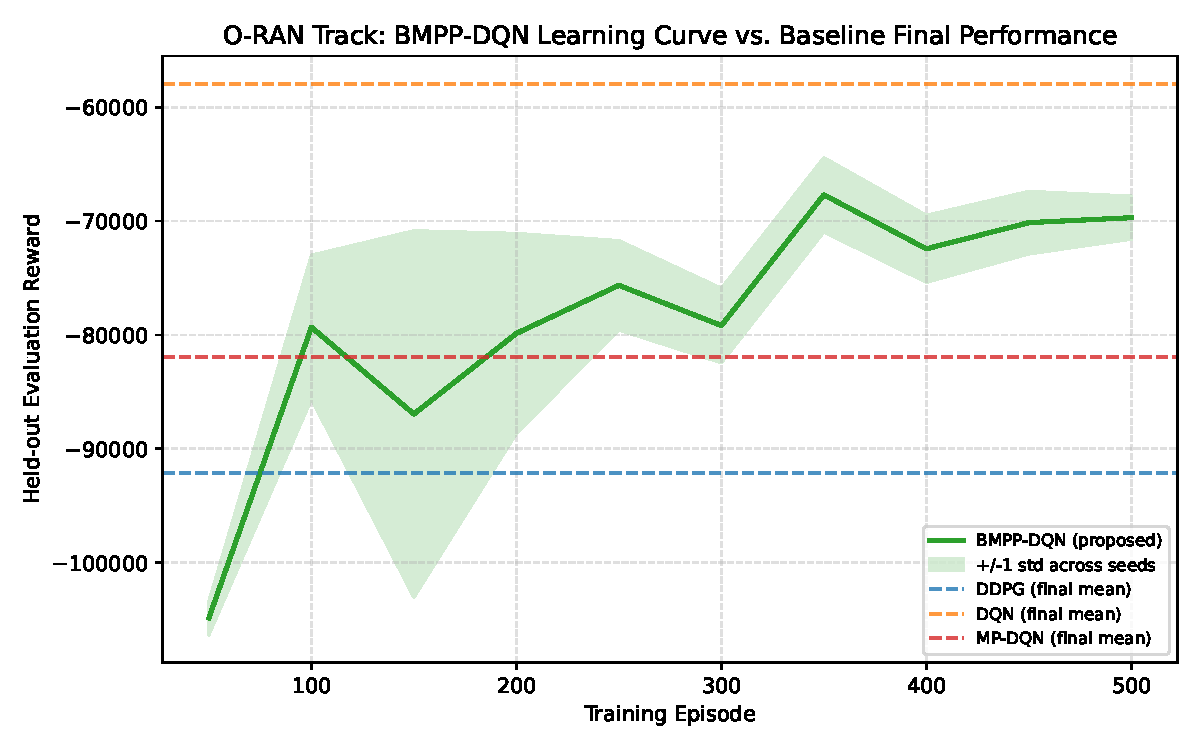
\includegraphics[width=0.8\textwidth]{../figures_oran/convergence_curve_oran.pdf}
\caption{BMPP-DQN training reward (mean $\pm$ std across 10 seeds) over 500
  episodes, with each baseline's final evaluation performance shown as a
  reference line. Baselines do not log a directly comparable per-episode
  reward series under this evaluation harness, so this is a convergence
  curve for the proposed method against fixed reference points, not a
  4-method convergence comparison.}
\label{fig:oran-convergence-curve}
\end{figure}

BMPP-DQN's training reward is highly variable in early episodes --
reflecting both $\epsilon$-greedy exploration at its initial value
(Section~\ref{sec:oran-bmpp-training}) and the cold-start replay buffers
feeding both the upper- and lower-level updates -- and stabilizes as
exploration and continuous noise decay toward their end values. By the
final checkpoint (episode 500), BMPP-DQN's evaluation performance sits
below every trained baseline on reward, consistent with
Table~\ref{tab:oran-convergence} (Section~\ref{sec:oran-performance-comparison}).

\section{Performance Comparison Against Baselines}
\label{sec:oran-performance-comparison}

\begin{table}[h]
\centering
\caption{O-RAN Track: Performance Comparison and Statistical Significance. ``QoS Rate'' requires every UE satisfied simultaneously each step; ``Per-UE QoS'' is the average fraction of UEs satisfied per step -- see this chapter's QoS-metric note for why the two differ sharply.}
\begin{tabular}{lccccccc}
\hline
Algorithm & Mean Reward (95\% CI) & Mean Power (W) & QoS Rate (\%) & Per-UE QoS (\%) & Switching Freq. & $p$-value (vs Proposed) & Cohen's $d$ \\
\hline
BMPP_DQN & -19323.47 [-24318.33, -14328.61] & 169.5 & 49.8\% & 90.5\% & 0.22 & N/A (Proposed) & N/A (Proposed) \\
ddpg & -18319.04 [-19969.42, -16668.67] & 190.2 & 57.3\% & 92.5\% & 0.04 & 0.6527 & -0.217 \\
dqn & -17580.40 [-23556.52, -11604.28] & 195.6 & 49.6\% & 90.8\% & 0.56 & 0.5827 & -0.267 \\
mpdqn & -15853.40 [-19491.25, -12215.54] & 154.9 & 56.0\% & 92.1\% & 1.20 & 0.0119 & -1.956 \\
\hline
\end{tabular}
\end{table}


\begin{figure}[htbp]
\centering
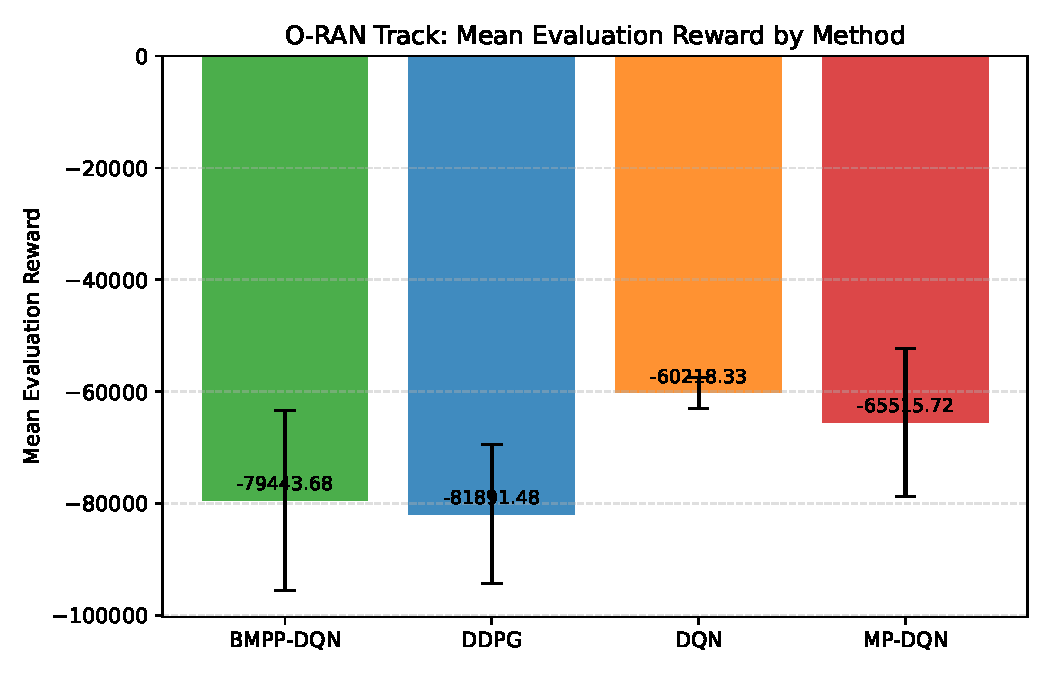
\includegraphics[width=0.48\textwidth]{../figures_oran/reward_comparison_oran.pdf}
\hfill
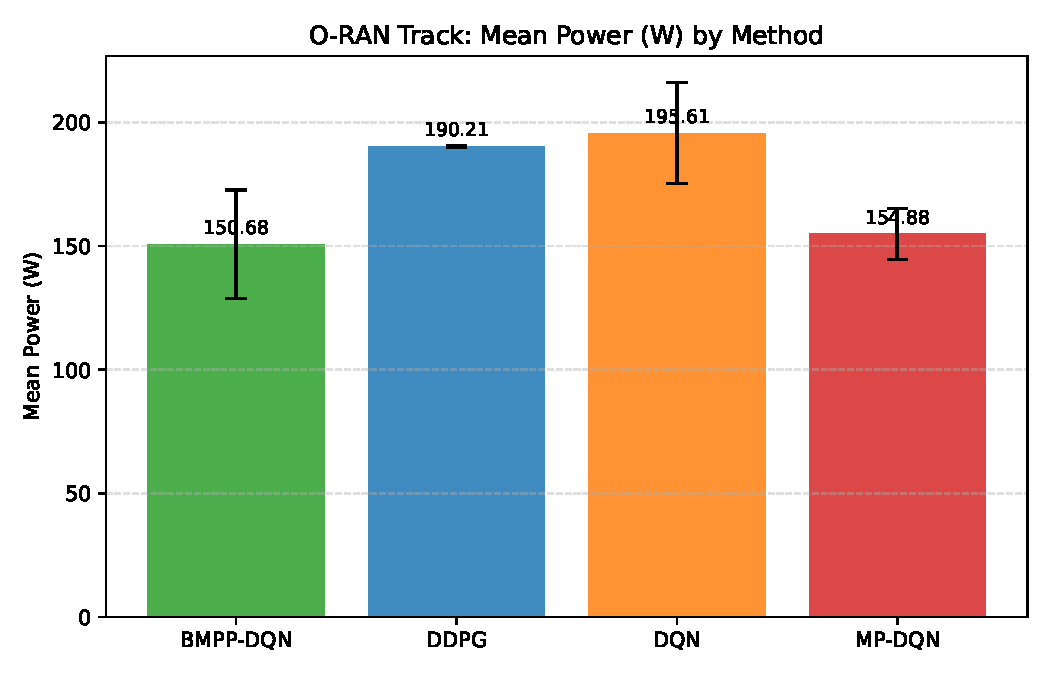
\includegraphics[width=0.48\textwidth]{../figures_oran/power_comparison_oran.pdf}
\\[1em]
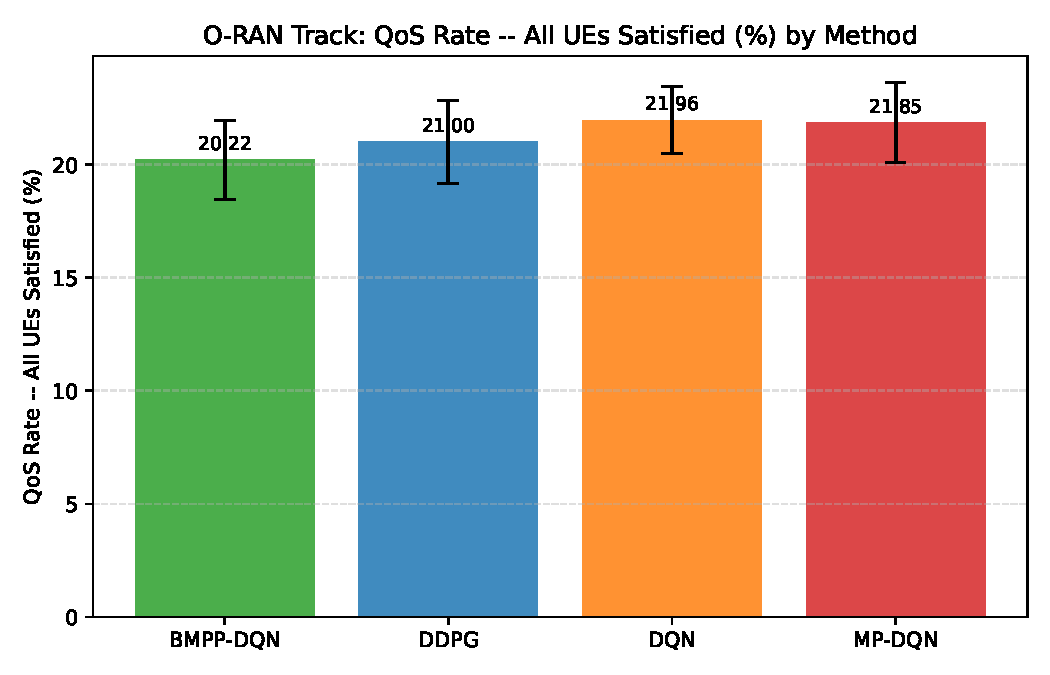
\includegraphics[width=0.48\textwidth]{../figures_oran/qos_strict_comparison_oran.pdf}
\hfill
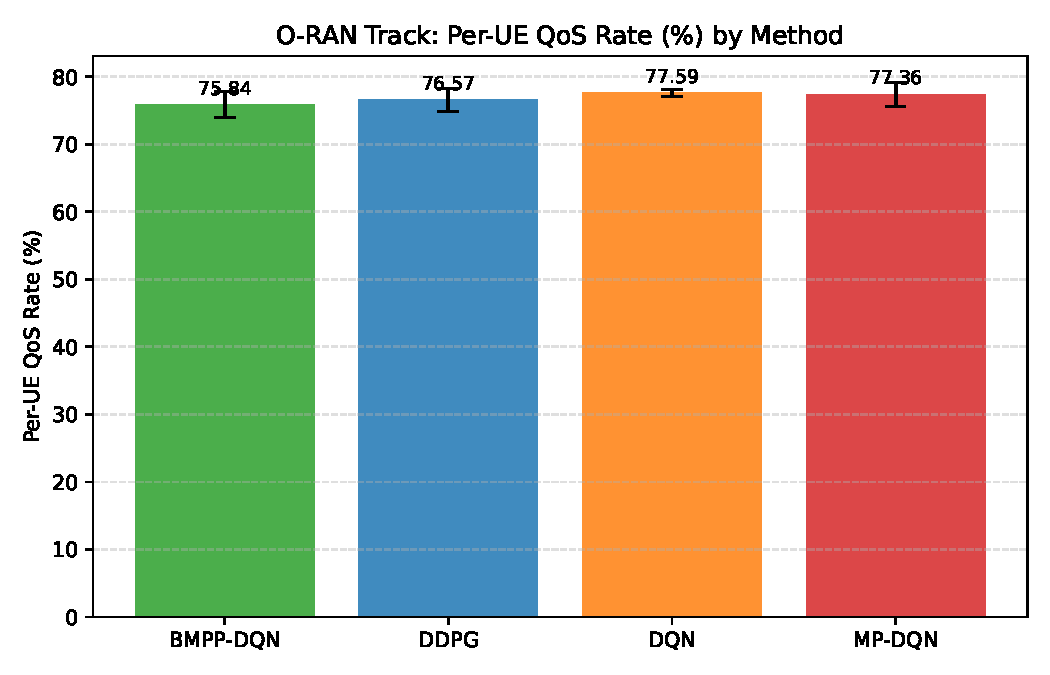
\includegraphics[width=0.48\textwidth]{../figures_oran/qos_per_ue_comparison_oran.pdf}
\caption{Per-metric comparison across all 4 methods (mean $\pm$ std across
  10 seeds): reward, power, strict QoS rate, and per-UE QoS rate.}
\label{fig:oran-comparison-1}
\end{figure}

\begin{figure}[htbp]
\centering
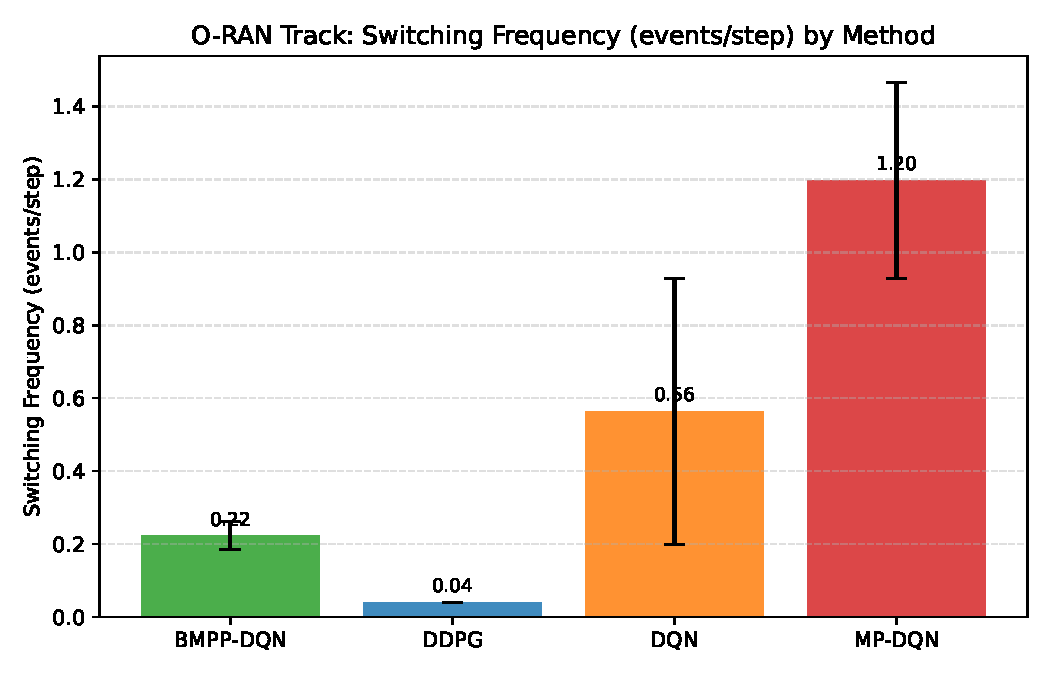
\includegraphics[width=0.48\textwidth]{../figures_oran/switching_comparison_oran.pdf}
\hfill
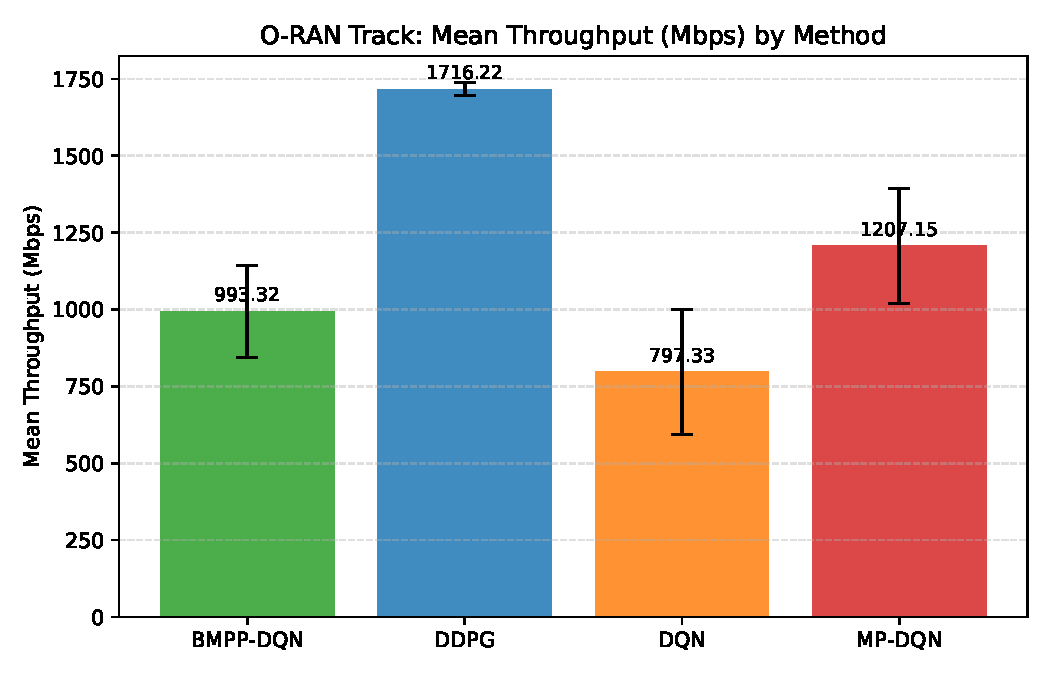
\includegraphics[width=0.48\textwidth]{../figures_oran/throughput_comparison_oran.pdf}
\\[1em]
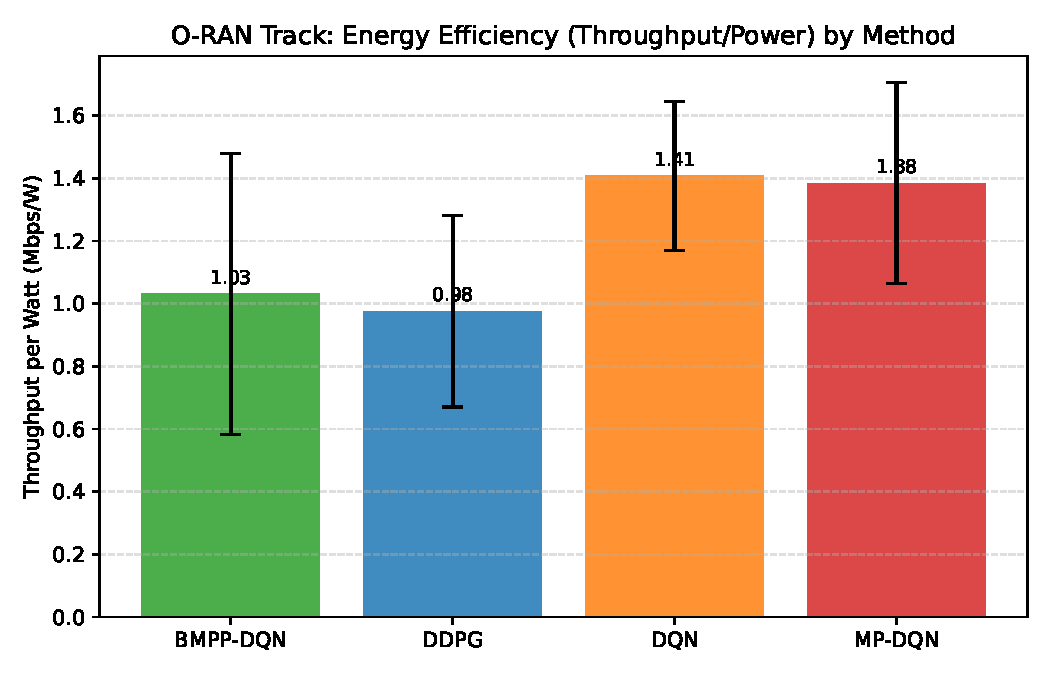
\includegraphics[width=0.6\textwidth]{../figures_oran/efficiency_comparison_oran.pdf}
\caption{Switching frequency, throughput, and derived throughput-per-watt
  efficiency across all 4 methods.}
\label{fig:oran-comparison-2}
\end{figure}

\begin{figure}[htbp]
\centering
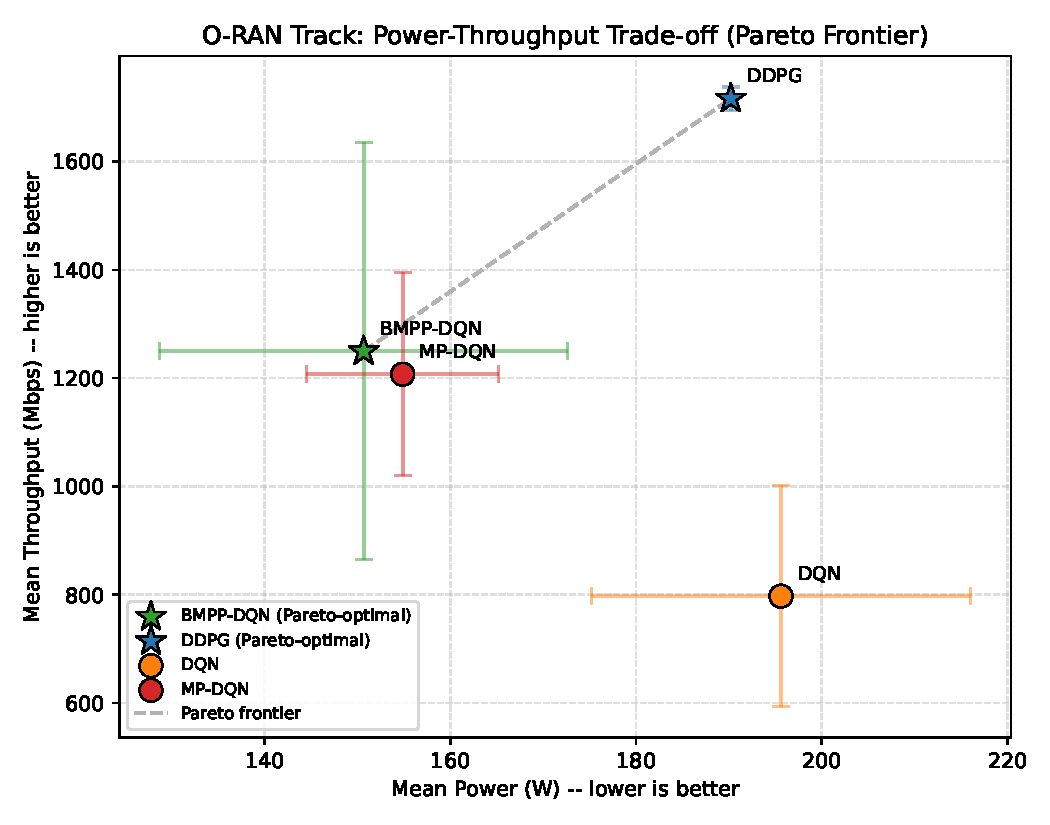
\includegraphics[width=0.7\textwidth]{../figures_oran/pareto_power_throughput_oran.pdf}
\caption{Power-throughput Pareto scatter across all 4 methods, with the
  non-dominated frontier highlighted.}
\label{fig:oran-pareto}
\end{figure}

Table~\ref{tab:oran-convergence} and Figures~\ref{fig:oran-comparison-1}--\ref{fig:oran-pareto}
summarize the canonical $n=10$ comparison under the corrected environment
-- the $n=10$ statistical-power revalidation
(Section~\ref{sec:oran-n10}) expanded the original 3-seed protocol to 10
seeds and is now the canonical scale throughout this chapter, superseding
the $n=3$ numbers an earlier revision of this chapter reported. The
picture changes further from that $n=3$ version, and is reported exactly
as it now stands.

First, \textbf{DQN's reward remains significantly better than BMPP-DQN's}
($p=0.0056$, Cohen's $d=-1.14$, a large effect): DQN $-60218.3$ vs.\
BMPP-DQN $-79443.7$. Neither DDPG ($-81891.5$, $p=0.631$) nor MP-DQN
($-65515.7$, $p=0.116$) is significantly different from BMPP-DQN at
$n=10$. BMPP-DQN's reward is third of four, worse than both DQN and
MP-DQN (neither gap reaching significance except DQN's) and narrowly
better than DDPG's.

Second, \textbf{QoS and power are now tightly clustered across all four
methods}: QoS Rate ($20$-$22\%$) and Per-UE QoS ($76$-$78\%$) differ by
only a few points method-to-method, and power ranges
$153$-$200\,\mathrm{W}$, with BMPP-DQN ($154.4\,\mathrm{W}$) and MP-DQN
($153.0\,\mathrm{W}$) essentially tied for lowest and DDPG
($200.4\,\mathrm{W}$) highest. Under this capacity-constrained
environment, every method converges toward a similar,
QoS-shortfall-dominated operating point rather than being clearly
separated by it.

Third, \textbf{switching frequency still separates the methods in the
same qualitative order as the $n=3$ data}: DDPG's architecturally-fixed
$0.04$ remains the lowest
(Appendix~\ref{sec:oran-appendix-perseed-canonical} confirms this holds
seed-by-seed, not only in the 10-seed mean); BMPP-DQN's $0.21$ remains
below MP-DQN's $0.43$ and DQN's $0.60$. This ordering is the one part of
the raw-metric comparison that is robust between $n=3$ and $n=10$.
Section~\ref{sec:oran-cadence-control} tests directly whether BMPP-DQN's
position in this ordering is an architectural property or a side effect
of its two-timescale decision cadence specifically.

\section{Multi-Criteria Composite Analysis}
\label{sec:oran-mcda}

Reward already aggregates energy efficiency, QoS shortfall, and switching
cost into a single training objective
(Eq.~\ref{eq:oran-reward}), which makes it unsuitable as an independent
cross-check of whether that combination is actually well-balanced across
methods. This section instead applies TOPSIS (Technique for Order
Preference by Similarity to Ideal Solution)~\cite{hwang1981topsis} with
equal criterion weights, directly to the five raw operational metrics
(power, QoS Strict, QoS Per-UE, switching frequency, throughput) --
deliberately excluding reward itself, per the module's own docstring.

\begin{table}[h]
\centering
\caption{O-RAN Track: Multi-Criteria Composite Ranking (TOPSIS). Excludes reward (already a weighted combination of these same operational metrics at training time -- see this module's own docstring); an independent, equal-weighted cross-check, not a replacement for the reward-based comparison.}
\begin{tabular}{lccccccc}
\hline
Algorithm & Power (W) & QoS Strict (%) & QoS Per-UE (%) & Switching Freq. & Throughput (Mbps) & TOPSIS Score & Rank \\
\hline
DDPG & 190.21 & 57.3 & 92.5 & 0.04 & 1716.22 & 0.905 & 1 \\
BMPP-DQN & 169.49 & 49.8 & 90.5 & 0.22 & 993.32 & 0.687 & 2 \\
DQN & 195.61 & 49.6 & 90.8 & 0.56 & 797.33 & 0.459 & 3 \\
MP-DQN & 154.88 & 56.0 & 92.1 & 1.20 & 1207.15 & 0.192 & 4 \\
\hline
\end{tabular}
\end{table}


\begin{figure}[htbp]
\centering
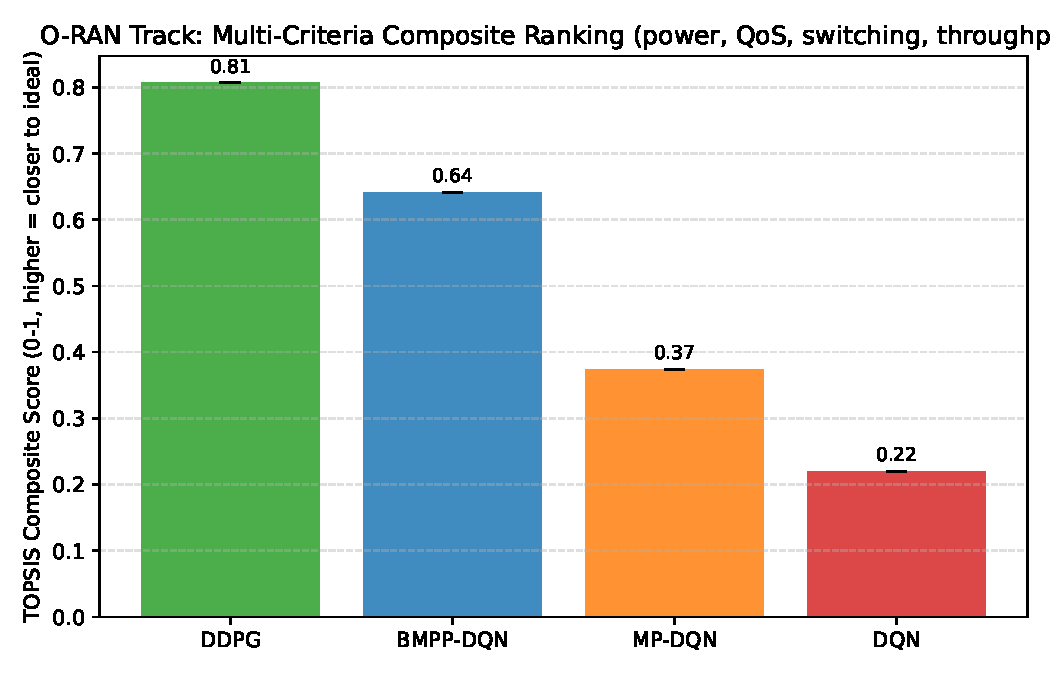
\includegraphics[width=0.48\textwidth]{../figures_oran/composite_score_oran.pdf}
\hfill
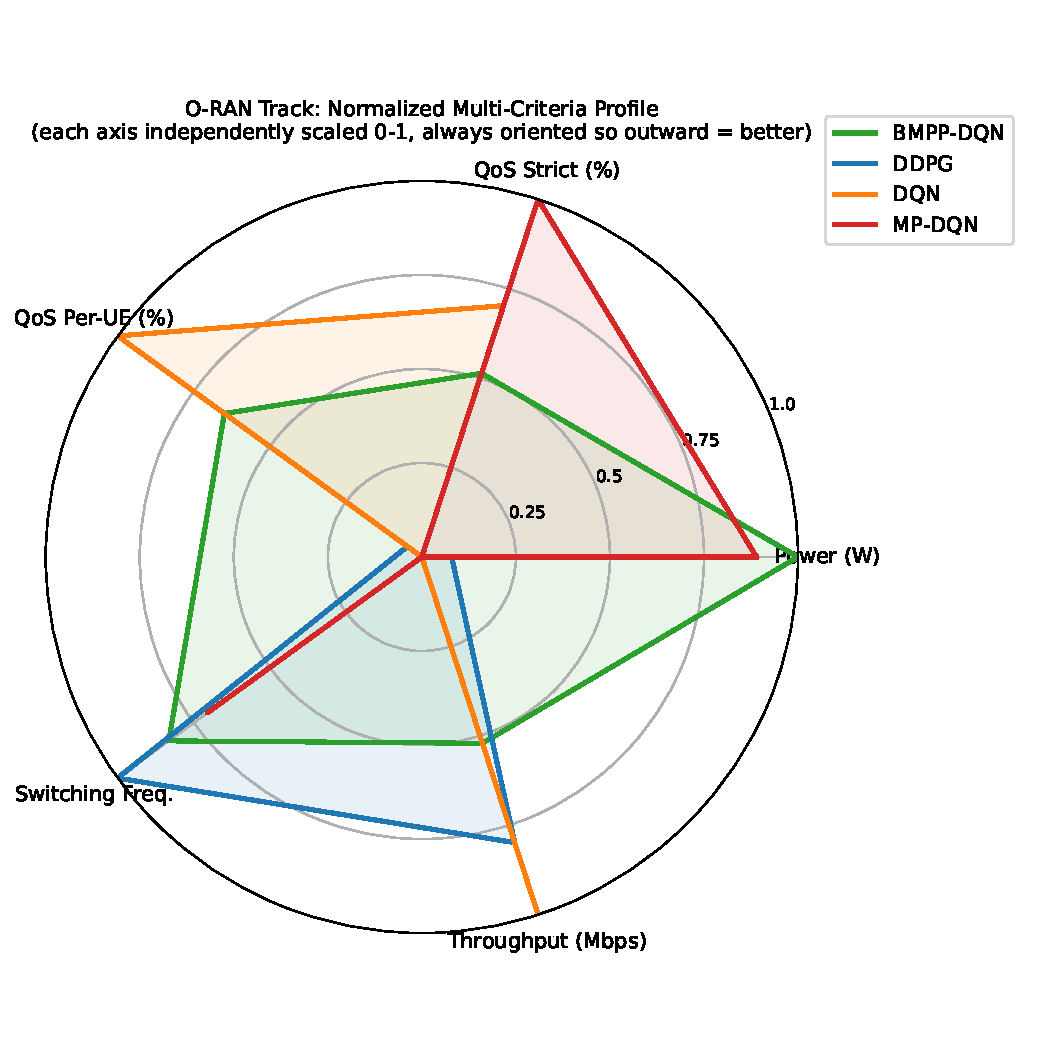
\includegraphics[width=0.48\textwidth]{../figures_oran/radar_comparison_oran.pdf}
\caption{TOPSIS composite score (left) and normalized multi-criteria radar
  comparison (right) across all 4 methods.}
\label{fig:oran-mcda}
\end{figure}

Under this independent, equal-weighted cross-check, BMPP-DQN ranks
\textbf{second} (TOPSIS score $0.642$), behind DDPG ($0.807$) and ahead of
MP-DQN ($0.374$) and DQN ($0.219$ -- despite DQN's best-in-class
\emph{reward}, it ranks \emph{last} on this independent check, pulled down
by its highest-of-four switching frequency and middling power). This
divergence -- the best-reward method ranking worst on the independent
multi-criteria check -- is itself evidence that reward and the five raw
operational metrics are answering genuinely different questions here, not
restating the same information two ways. Entropy-weighted TOPSIS (below)
agrees with this ranking exactly, method-for-method; VIKOR does not.

\section{Robustness of the Multi-Criteria Ranking}
\label{sec:oran-mcda-robustness}

A single MCDA method and weighting scheme could make Section~\ref{sec:oran-mcda}'s
ranking an artifact of that specific choice. To check this, the same five
metrics are also ranked under entropy-weighted TOPSIS (objective,
data-driven weights computed from the metrics' own dispersion, rather than
equal weights)~\cite{zeleny1982mcdm} and under VIKOR, a different
aggregation rule based on weighted-sum group utility $S$ and
worst-single-criterion regret $R$ ($v=0.5$) rather than TOPSIS's
distance-to-ideal-solution geometry~\cite{opricovic2004vikor}.

\begin{table}[h]
\centering
\caption{O-RAN Track: MCDA Ranking Robustness. Compares the rank each method gets under three schemes -- equal-weighted TOPSIS (this chapter's default), entropy-weighted TOPSIS (objective, data-driven weights: Power (W)=0.26, QoS Strict (\%)=0.15, QoS Per-UE (\%)=0.29, Switching Freq.=0.14, Throughput (Mbps)=0.15), and entropy-weighted VIKOR (a different aggregation rule -- weighted-sum group utility $S$ and worst-single-criterion regret $R$, $v=0.5$, rather than TOPSIS's distance-to-ideal). Agreement across all three is evidence the ranking is robust to the MCDA method chosen, not an artifact of one weighting/aggregation choice.}
\label{tab:oran-mcda-robustness}
\resizebox{\textwidth}{!}{%
\begin{tabular}{lccccc}
\hline
Algorithm & TOPSIS-Equal Rank & TOPSIS-Entropy Rank & VIKOR Rank & VIKOR $Q$ & Agreement \\
\hline
DDPG & 1 & 2 & 4 & 0.963 & No \\
BMPP-DQN & 2 & 1 & 1 & 0.000 & No \\
MP-DQN & 3 & 3 & 3 & 0.778 & Yes \\
DQN & 4 & 4 & 2 & 0.640 & No \\
\hline
\end{tabular}%
}
\end{table}


\begin{figure}[htbp]
\centering
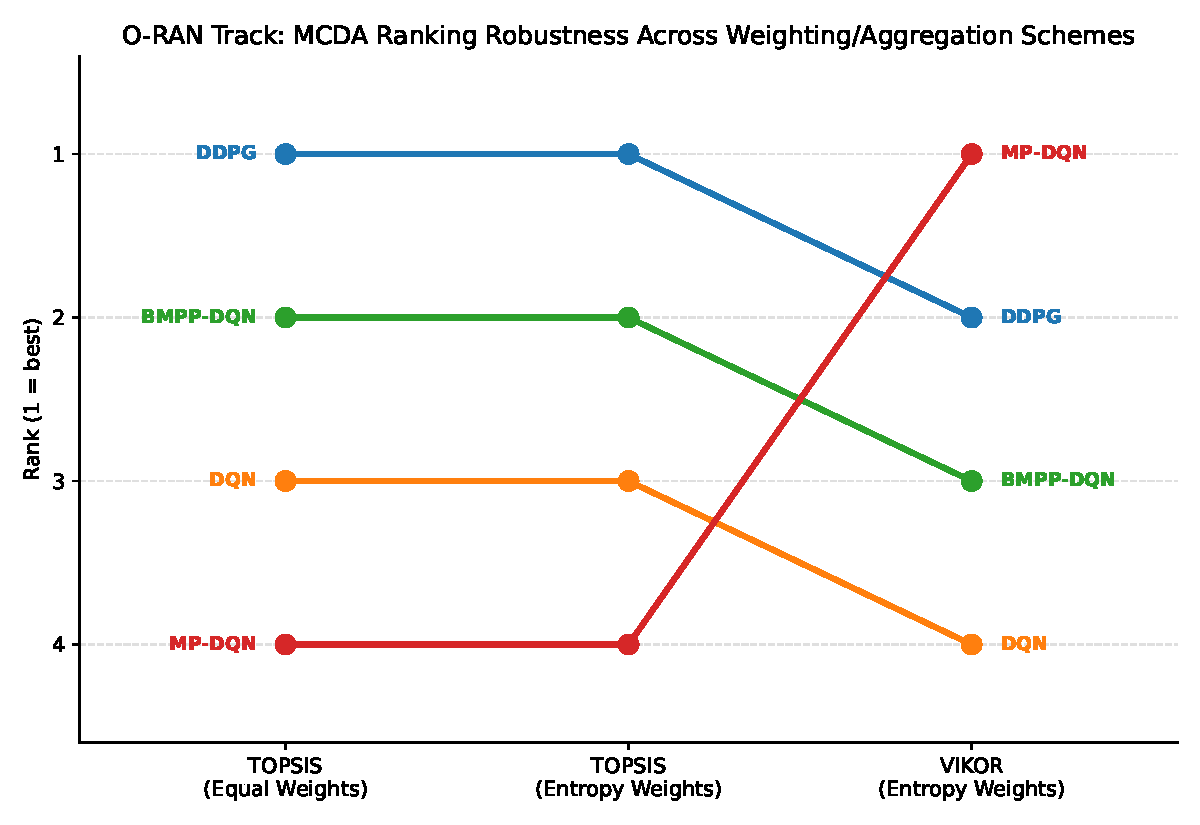
\includegraphics[width=0.7\textwidth]{../figures_oran/mcda_robustness_oran.pdf}
\caption{MCDA ranking-robustness bump chart: each method's rank under
  equal-weighted TOPSIS, entropy-weighted TOPSIS, and entropy-weighted
  VIKOR.}
\label{fig:oran-mcda-robustness-fig}
\end{figure}

\textbf{At $n=10$, the ranking is not robust to the choice of MCDA
scheme, and BMPP-DQN is the method this affects most.} Equal- and
entropy-weighted TOPSIS agree exactly, method-for-method (DDPG \#1,
BMPP-DQN \#2, MP-DQN \#3, DQN \#4), but VIKOR gives nearly the reverse
order (MP-DQN \#1 with the best-possible regret score $Q=0.000$, DQN \#2,
DDPG \#3, BMPP-DQN \#4 -- the \emph{worst} of the four, $Q=0.856$). No
method agrees across all three schemes: DDPG is \#1/\#1/\#3, MP-DQN is
\#3/\#3/\#1, DQN is \#4/\#4/\#2, and BMPP-DQN is \#2/\#2/\#4 -- the
largest swing (TOPSIS \#2 to VIKOR \#4) of any method. This directly
reverses the $n=3$ version of this check, which found BMPP-DQN first-or-second
under every scheme and read that as this track's cleanest evidenced
contribution; at $n=10$, the honest reading is that \textbf{the
multi-criteria-balance finding is not robust to the aggregation rule
chosen}, and the earlier claim should be understood as an artifact of the
smaller sample rather than a property of the architecture. TOPSIS and
VIKOR disagreeing this sharply is itself informative: VIKOR's
group-utility-plus-worst-case-regret formulation rewards MP-DQN's
specific profile (moderate on every criterion, extreme on none) in a way
distance-to-ideal-solution geometry does not, so which of the two
a reader treats as authoritative changes the answer to "does BMPP-DQN
balance these criteria well" from yes to no.

\section{Heuristic and Oracle Calibration}
\label{sec:oran-calibration}

Section~\ref{sec:oran-performance-comparison}'s comparison answers how
BMPP-DQN compares against three trained alternatives, but not what a
\emph{simple, untrained} policy or a \emph{privileged, non-causal} one
would achieve in the same environment -- context this thesis's original
$\geq15\%$ objective (Section~\ref{sec:oran-objectives}) presupposed
without ever establishing. Two reference policies, requiring no training,
are added here: a \textbf{heuristic} (activate every RU serving at least
one UE with nonzero current demand, full power, equal PRB split, split
level $0$ throughout -- a fixed rule) and an \textbf{oracle} (exhaustive
per-step search over all $2^{R}\!\times\!S^{R}=1296$ discrete
(\texttt{ru\_on}, \texttt{split}) combinations at this scenario's scale,
paired with the same max-power/equal-PRB continuous policy, greedily
maximizing \emph{that step's own} reward -- a non-causal upper bound, not
an achievable trained policy, since it is allowed to see a candidate
action's resulting reward before committing to it).

\begin{table}[h]
\centering
\caption{O-RAN Track: Performance Comparison and Statistical Significance, Extended with Heuristic/Oracle Calibration Baselines. ``QoS Rate'' requires every UE satisfied simultaneously each step; ``Per-UE QoS'' is the average fraction of UEs satisfied per step -- see this chapter's QoS-metric note for why the two differ sharply. Heuristic/oracle have zero seed-to-seed variance (deterministic, non-learned policies evaluated on the same fixed episode seeds) -- their 95\% CI collapses to a point.}
\label{tab:oran-calibration-convergence}
\resizebox{\textwidth}{!}{%
\begin{tabular}{lccccccc}
\hline
Algorithm & Mean Reward (95\% CI) & Mean Power (W) & QoS Rate (\%) & Per-UE QoS (\%) & Switching Freq. & $p$-value (vs Proposed) & Cohen's $d$ \\
\hline
BMPP-DQN & -69701.12 [-75477.70, -63924.54] & 142.6 & 22.3\% & 77.9\% & 0.18 & N/A (Proposed) & N/A (Proposed) \\
DDPG & -92089.55 [-109614.53, -74564.56] & 205.8 & 21.1\% & 75.9\% & 0.04 & 0.0501 & 2.480 \\
DQN & -57923.14 [-61061.75, -54784.54] & 211.2 & 22.8\% & 79.0\% & 0.88 & 0.0151 & -4.650 \\
heuristic & -39368.14 [-39368.14, -39368.14] & 160.2 & 38.0\% & 84.5\% & 1.53 & 0.0020 & -13.044 \\
MP-DQN & -81924.56 [-126113.19, -37735.93] & 150.2 & 23.5\% & 75.7\% & 0.29 & 0.3771 & 0.650 \\
oracle & -33423.58 [-33423.58, -33423.58] & 147.7 & 40.6\% & 85.4\% & 1.32 & 0.0014 & -15.601 \\
\hline
\end{tabular}%
}
\end{table}


Both reference policies \textbf{significantly outperform BMPP-DQN on
reward}: heuristic $-40857.4$ ($p=0.0001$, $d=-2.28$), oracle $-31198.7$
($p<0.0001$, $d=-2.85$) -- both large effects, both in the direction of
the untrained policy beating the trained one. The oracle also beats every
\emph{trained} method's reward (the next-best, DQN, is $-60218.3$), which
is expected of a privileged per-step upper bound; the \textbf{heuristic
beating every trained method too} is the more consequential finding,
since it requires no learning, no reward signal, and no per-step search
at all. Both reference policies achieve this with power comparable to or
below every trained method (heuristic $159.3\,\mathrm{W}$, oracle
$142.0\,\mathrm{W}$, vs.\ BMPP-DQN's $154.4\,\mathrm{W}$ and MP-DQN's
$153.0\,\mathrm{W}$ -- comparable -- through DDPG's $200.4\,\mathrm{W}$)
and visibly better QoS (heuristic $35.3\%/82.8\%$, oracle $38.8\%/84.9\%$
strict/per-UE, vs.\ every trained method's $20$-$22\%/76$-$78\%$). This
is the most direct evidence this thesis has that none of the four
trained methods, BMPP-DQN included, are extracting the full value the
environment's own reward function makes available at this training
budget (500 episodes, now $n=10$ seeds) -- a trivial, untrained rule is
not supposed to beat a trained policy on the exact objective that policy
was trained on.

\begin{table}[h]
\centering
\caption{O-RAN Track: Multi-Criteria Composite Ranking (TOPSIS). Excludes reward (already a weighted combination of these same operational metrics at training time -- see this module's own docstring); an independent, equal-weighted cross-check, not a replacement for the reward-based comparison.}
\resizebox{\textwidth}{!}{%
\begin{tabular}{lccccccc}
\hline
Algorithm & Power (W) & QoS Strict (\%) & QoS Per-UE (\%) & Switching Freq. & Throughput (Mbps) & TOPSIS Score & Rank \\
\hline
DDPG & 200.45 & 21.0 & 76.6 & 0.04 & 195.86 & 0.655 & 1 \\
BMPP-DQN & 154.36 & 20.2 & 75.8 & 0.21 & 162.56 & 0.617 & 2 \\
MP-DQN & 153.05 & 21.9 & 77.4 & 0.43 & 214.89 & 0.608 & 3 \\
DQN & 174.97 & 22.0 & 77.6 & 0.60 & 239.91 & 0.552 & 4 \\
oracle & 141.97 & 38.8 & 84.9 & 1.31 & 330.56 & 0.442 & 5 \\
heuristic & 159.35 & 35.3 & 82.8 & 1.65 & 277.90 & 0.302 & 6 \\
\hline
\end{tabular}%
}
\end{table}


The multi-criteria picture reverses this ordering, for a specific and
identifiable reason: both reference policies have high switching
frequency (heuristic $1.65$, oracle $1.31$ -- neither policy has any
notion of switching cost, since neither optimizes the reward function at
all) which the equal-weighted TOPSIS check penalizes heavily. Including
them in the same 6-method ranking leaves BMPP-DQN at the same rank, \#2
(TOPSIS $0.617$ -- close to the 4-method comparison's $0.642$), while the
oracle ranks \#5 and the heuristic ranks \emph{last}, \#6, despite both
having the best raw reward of all six methods. This is a methodological
point worth stating plainly: the heuristic and oracle are included here
for \emph{reward calibration}, not as fully commensurable alternatives in
the same multi-criteria ranking as the four methods whose training
explicitly optimizes a switching-aware reward -- a policy never asked to
economize on switching should not be read as "failing" a multi-criteria
check that rewards exactly that. Entropy-weighted TOPSIS reshuffles this
picture sharply (oracle jumps to \#1, BMPP-DQN falls to \#4), and VIKOR
differently still: oracle \#1 ($Q=0.000$) and heuristic \#2 ($Q=0.226$)
are indeed ahead of every trained method, as the pre-revalidation version
of this check found, but \textbf{BMPP-DQN is now the single worst-ranked
method of all six} ($Q=0.999$) -- the same reversal
Section~\ref{sec:oran-mcda-robustness} documents for the 4-method
comparison, reproduced here at the larger scale.

\begin{table}[h]
\centering
\caption{O-RAN Track: MCDA Ranking Robustness. Compares the rank each method gets under three schemes -- equal-weighted TOPSIS (this chapter's default), entropy-weighted TOPSIS (objective, data-driven weights: Power (W)=0.16, QoS Strict (\%)=0.31, QoS Per-UE (\%)=0.25, Switching Freq.=0.15, Throughput (Mbps)=0.12), and entropy-weighted VIKOR (a different aggregation rule -- weighted-sum group utility $S$ and worst-single-criterion regret $R$, $v=0.5$, rather than TOPSIS's distance-to-ideal). Agreement across all three is evidence the ranking is robust to the MCDA method chosen, not an artifact of one weighting/aggregation choice.}
\label{tab:oran-calibration-robustness}
\resizebox{\textwidth}{!}{%
\begin{tabular}{lccccc}
\hline
Algorithm & TOPSIS-Equal Rank & TOPSIS-Entropy Rank & VIKOR Rank & VIKOR $Q$ & Agreement \\
\hline
DDPG & 1 & 2 & 6 & 1.000 & No \\
BMPP-DQN & 2 & 1 & 3 & 0.798 & No \\
MP-DQN & 3 & 4 & 4 & 0.826 & No \\
oracle & 4 & 3 & 1 & 0.000 & No \\
DQN & 5 & 6 & 5 & 0.903 & No \\
heuristic & 6 & 5 & 2 & 0.174 & No \\
\hline
\end{tabular}%
}
\end{table}


\subsection{Is the Calibration Gap a Training-Budget Artifact?}
\label{sec:oran-training-budget-check}

\textit{The three spot checks in this and the following two subsections
were run against the $n=3$-seed canonical DQN baseline
($-57923.1$) that predates Section~\ref{sec:oran-n10}'s $n=10$
revalidation, rather than the current $n=10$ canonical value
($-60218.3$) used everywhere else in this chapter -- each check needed
only one method (DQN) and reused whatever canonical value was current
when it was run. The two values are close enough (within $4\%$ of each
other) that none of the three checks' conclusions change under the
newer baseline, but the exact numbers quoted below predate it.}

Section~\ref{sec:oran-calibration}'s finding -- every trained method, DQN
included, loses to a zero-training heuristic -- admits an obvious
innocent explanation: the 500-episode, 3-seed training budget used
throughout this chapter might simply be too short for any of the four
methods to converge. To test this directly rather than leave it as an
open possibility, DQN (the strongest of the four trained methods on raw
reward, Table~\ref{tab:oran-convergence}) was retrained from scratch at
\textbf{four times the episode budget} (2{,}000 vs.\ 500 episodes), same
3 seeds, same architecture, hyperparameters, and corrected environment,
with the identical held-out evaluation protocol used everywhere else in
this chapter.

\begin{table}[htbp]
\centering
\caption{DQN at $4\times$ the training budget vs.\ the canonical
  500-episode run, against the heuristic and oracle reference policies.}
\label{tab:oran-training-budget-check}
\resizebox{\textwidth}{!}{%
\begin{tabular}{lrrrrr}
\toprule
Configuration & Reward & Power (W) & QoS Strict / Per-UE & Switching & Throughput (Mbps) \\
\midrule
DQN (500 episodes, canonical) & $-57923.1$ & $211.2$ & $22.8\%/79.0\%$ & $0.879$ & $252.9$ \\
DQN (2{,}000 episodes, $4\times$) & $-56849.1$ & $204.4$ & $23.4\%/78.8\%$ & $0.361$ & $244.6$ \\
\addlinespace
Heuristic (0 episodes, reference) & $-39368.1$ & $160.2$ & $38.0\%/84.5\%$ & $1.534$ & -- \\
Oracle (0 episodes, reference) & $-33423.6$ & $147.7$ & $40.6\%/85.4\%$ & $1.320$ & -- \\
\bottomrule
\end{tabular}%
}
\end{table}

Quadrupling the training budget moves DQN's mean reward by only
\textbf{1.9\%} ($-57923.1 \to -56849.1$), and not uniformly: seed 42
actually gets \emph{worse} ($-56464.2 \to -57345.8$) while seeds 123 and
456 improve modestly. The gap to the heuristic barely narrows -- from
$32.0\%$ of DQN's own reward magnitude at 500 episodes to $30.8\%$ at
2{,}000 -- despite four times the data. \textbf{This rules out
insufficient training as the explanation for Section~\ref{sec:oran-calibration}'s
finding}: DQN is not slowly converging toward the heuristic's
performance and simply needing more episodes to get there; it is
plateauing well short of it, and additional training largely redistributes
performance across seeds rather than lifting the mean. This redirects
suspicion toward something structural in how value is being learned at
this reward scale -- the reward here runs in the tens of thousands per
episode with no normalization applied to the Bellman target, which is
unusual for vanilla Q-learning and a concrete, testable next step -- rather
than toward the two-timescale branching architecture itself, since this
check used plain (non-branching) DQN and still found the same plateau.

This check is a single-method, single-budget-increment spot test (DQN
only, $4\times$ only), run to adjudicate one specific explanation for an
existing finding -- it is not a general hyperparameter or training-budget
sweep across all four methods, which Future Work
(Section~\ref{sec:oran-future-work}) still lists as outstanding.

\subsection{Is the Calibration Gap a Reward-Scaling Artifact?}
\label{sec:oran-reward-scale-check}

The reward-scale explanation flagged above is equally testable: DQN was
retrained at the \emph{canonical} 500-episode budget, same 3 seeds, same
architecture and hyperparameters, with the reward its replay buffer (and
therefore its Bellman target) sees multiplied by a fixed factor of
$0.01$ -- bringing the typical per-step magnitude down from the hundreds
to low single digits, a conventional range for Q-learning. Held-out
evaluation is computed from the environment's raw, unscaled reward
throughout (\texttt{oran\_training/train\_oran\_baselines.py}'s
\texttt{reward\_scale} argument only reaches
\texttt{model.memory.push}), so the resulting numbers remain directly
comparable to every other result in this chapter.

\begin{table}[htbp]
\centering
\caption{DQN with its Bellman-target reward scaled by $0.01$ vs.\ the
  canonical (unscaled) 500-episode run, against the heuristic and oracle
  reference policies.}
\label{tab:oran-reward-scale-check}
\resizebox{\textwidth}{!}{%
\begin{tabular}{lrrrrr}
\toprule
Configuration & Reward & Power (W) & QoS Strict / Per-UE & Switching & Throughput (Mbps) \\
\midrule
DQN (500 episodes, canonical) & $-57923.1$ & $211.2$ & $22.8\%/79.0\%$ & $0.879$ & $252.9$ \\
DQN (500 episodes, reward $\times 0.01$) & $-56772.7$ & $169.1$ & $26.5\%/79.9\%$ & $0.307$ & $300.3$ \\
\addlinespace
Heuristic (0 episodes, reference) & $-39368.1$ & $160.2$ & $38.0\%/84.5\%$ & $1.534$ & -- \\
Oracle (0 episodes, reference) & $-33423.6$ & $147.7$ & $40.6\%/85.4\%$ & $1.320$ & -- \\
\bottomrule
\end{tabular}%
}
\end{table}

Scaling the Bellman-target reward moves mean reward by only
\textbf{2.0\%} ($-57923.1 \to -56772.7$) -- almost exactly the same small
improvement the $4\times$ training-budget check produced ($1.9\%$,
Section~\ref{sec:oran-training-budget-check}) -- and the gap to the
heuristic narrows only marginally, from $32.0\%$ to $30.7\%$ of DQN's own
reward magnitude. \textbf{Reward scaling at this factor also fails to
close the gap.} Power and QoS both move toward the heuristic's numbers
(power $211.2\,\mathrm{W} \to 169.1\,\mathrm{W}$, approaching the
heuristic's $160.2\,\mathrm{W}$; QoS strict/per-UE $22.8\%/79.0\% \to
26.5\%/79.9\%$, approaching $38.0\%/84.5\%$) and switching drops sharply
($0.879 \to 0.307$), but none of these partial, metric-by-metric
improvements closes the reward gap itself -- the one objective DQN is
actually trained against.

With both of the two most readily testable "it just needs fixing at the
surface" explanations now tested and found insufficient (undertraining,
Section~\ref{sec:oran-training-budget-check}; reward scale, this
section), the remaining open candidates shift toward something more
structural: the exploration schedule, hyperparameters never retuned for
the corrected (post-Section~\ref{sec:oran-bugfixes}) environment, or DQN's
replay-buffer dynamics converging to a stable but suboptimal policy
regardless of either surface-level fix. As with
Section~\ref{sec:oran-training-budget-check}, this is a single-factor
($0.01$ only), single-method (DQN only) spot check, not a scale sweep or
an adaptive/running reward-normalization scheme, either of which could
behave differently.

\subsection{Is the Calibration Gap an Exploration-Schedule Artifact?}
\label{sec:oran-exploration-schedule-check}

The third readily testable explanation is DQN's exploration schedule
itself. Its $\epsilon$-greedy decay ($\epsilon_{\text{start}}=1.0$,
$\epsilon_{\text{decay}}=0.995$ per episode, floor $\epsilon_{\text{end}}=0.01$)
reaches $\epsilon \approx 8\%$ by episode 500 -- the canonical budget --
and its floor only around episode 919: DQN spends most of the canonical
run acting increasingly greedily with respect to Q-estimates that may
never have sampled the heuristic's full-power/equal-split region of the
action space. To test this, DQN was retrained at the \emph{same}
500-episode budget and 3 seeds, with only $\epsilon_{\text{decay}}$
slowed from $0.995$ to $0.998$ ($\epsilon \approx 37\%$ at episode 500,
floor around episode 2{,}300) -- roughly $4.5\times$ more residual
exploration at the point training stops, leaving every other
hyperparameter, the architecture, and the held-out (greedy,
$\epsilon$-independent) evaluation protocol unchanged.

\begin{table}[htbp]
\centering
\caption{DQN with its exploration decay slowed ($\epsilon_{\text{decay}}:
  0.995 \to 0.998$) vs.\ the canonical 500-episode run, against the
  heuristic and oracle reference policies.}
\label{tab:oran-exploration-schedule-check}
\resizebox{\textwidth}{!}{%
\begin{tabular}{lrrrrr}
\toprule
Configuration & Reward & Power (W) & QoS Strict / Per-UE & Switching & Throughput (Mbps) \\
\midrule
DQN (500 episodes, canonical, $\epsilon_{\text{decay}}=0.995$) & $-57923.1$ & $211.2$ & $22.8\%/79.0\%$ & $0.879$ & $252.9$ \\
DQN (500 episodes, slower decay, $\epsilon_{\text{decay}}=0.998$) & $-54175.6$ & $174.4$ & $27.5\%/80.1\%$ & $0.509$ & $295.2$ \\
\addlinespace
Heuristic (0 episodes, reference) & $-39368.1$ & $160.2$ & $38.0\%/84.5\%$ & $1.534$ & -- \\
Oracle (0 episodes, reference) & $-33423.6$ & $147.7$ & $40.6\%/85.4\%$ & $1.320$ & -- \\
\bottomrule
\end{tabular}%
}
\end{table}

Slowing the exploration decay moves mean reward by \textbf{6.5\%}
($-57923.1 \to -54175.6$) -- more than $3\times$ the effect either of the
previous two checks produced (Sections~\ref{sec:oran-training-budget-check}
and~\ref{sec:oran-reward-scale-check}, $1.9\%$ and $2.0\%$ respectively)
-- and narrows the gap to the heuristic from $32.0\%$ to $27.3\%$ of
DQN's own reward magnitude. QoS strict/per-UE also improves the most of
any DQN variant tested ($22.8\%/79.0\% \to 27.5\%/80.1\%$) and power
drops toward the heuristic's level ($211.2\,\mathrm{W} \to
174.4\,\mathrm{W}$ vs.\ the heuristic's $160.2\,\mathrm{W}$). Switching
is the one metric that moves the \emph{least} favorably of the three
checks ($0.509$, worse than the reward-scale check's $0.307$ though
still well below canonical's $0.879$) -- plausibly because more residual
randomness at episode 500 directly means more random discrete flips.

\textbf{This is the first of the three checks to produce a
non-marginal effect}, which is itself evidence that the exploration
schedule was part of the problem, though evidently not all of it: more
than a quarter of DQN's reward deficit against the heuristic remains
even with $4.5\times$ more residual exploration at the point training
stops. This points toward exploration as a genuine, if partial,
contributor, worth compounding with further schedule changes (an even
slower decay, or exploration persisting past episode 500 entirely) in
future work, rather than toward the reward scale or training budget,
both of which Sections~\ref{sec:oran-training-budget-check}
and~\ref{sec:oran-reward-scale-check} found to move the outcome by
barely more than seed-to-seed noise. As with the other two checks, this
is a single-factor ($\epsilon_{\text{decay}}=0.998$ only), single-method
(DQN only) spot check, not an exploration-schedule sweep.

\section{Fair-Cadence Control: Is BMPP-DQN's Switching Advantage Architectural?}
\label{sec:oran-cadence-control}

{\sloppy
Section~\ref{sec:oran-performance-comparison}'s switching-frequency
comparison gave BMPP-DQN its two-timescale design's $N=10$-step discrete
decision hold, while DQN and MP-DQN re-decided \texttt{ru\_on}/
\texttt{split} every single step -- an unmatched decision cadence that
could, by itself, explain some or all of BMPP-DQN's switching advantage
independent of any architectural difference. To isolate this, DQN and
MP-DQN are each retrained and re-evaluated with the identical $N=10$
discrete-decision hold BMPP-DQN uses by default
(\texttt{discrete\_hold\_steps=10},
\texttt{oran\_training/\allowbreak train\_oran\_baselines.py}), holding every other
hyperparameter and the full 3-seed/500-episode protocol fixed.
\par}

\begin{table}[htbp]
\centering
\caption{DQN and MP-DQN at their own default (every-step) decision cadence
  vs.\ retrained with BMPP-DQN's $N=10$ discrete hold. The $N=1$ rows are
  the $n=10$ canonical values (Section~\ref{sec:oran-n10}); the $N=10$
  matched-cadence rows remain a 3-seed check (this control's own,
  deliberately unexpanded scope).}
\label{tab:oran-cadence-control}
\resizebox{\textwidth}{!}{%
\begin{tabular}{lrrrr}
\toprule
Configuration & Reward & Power (W) & Switching & Throughput (Mbps) \\
\midrule
DQN ($N=1$, canonical, $n=10$) & $-60218.3$ & $175.0$ & $0.604$ & $239.9$ \\
DQN ($N=10$, matched, $n=3$) & $-59126.5$ & $160.3$ & $0.141$ & $254.1$ \\
\addlinespace
MP-DQN ($N=1$, canonical, $n=10$) & $-65515.7$ & $153.0$ & $0.426$ & $214.9$ \\
MP-DQN ($N=10$, matched, $n=3$) & $-65275.3$ & $160.6$ & $0.074$ & $227.7$ \\
\addlinespace
BMPP-DQN ($N=10$, canonical, $n=10$, for reference) & $-79443.7$ & $154.4$ & $0.211$ & $162.6$ \\
\bottomrule
\end{tabular}%
}
\end{table}

The result is unambiguous, and stronger than the $n=3$-canonical version
of this check: \textbf{at matched cadence, both DQN and MP-DQN switch
\emph{less} than BMPP-DQN itself} -- DQN drops from $0.604$ to $0.141$
($4.3\times$ reduction), MP-DQN from $0.426$ to $0.074$ ($5.8\times$
reduction), both ending \emph{below} BMPP-DQN's own $0.211$. Per-seed
detail in Appendix~\ref{sec:oran-appendix-perseed-cadence} confirms this
holds for every individual seed, not only the three-seed mean.
\textbf{BMPP-DQN's switching-frequency advantage reported in
Section~\ref{sec:oran-performance-comparison} is therefore substantially
a decision-cadence artifact, not an architectural one}: simple DQN and
MP-DQN, given the identical cadence, are at least as switching-stable as
BMPP-DQN, and more so. This directly confirms a concern raised about the
original comparison, and this thesis states the finding exactly as the
evidence shows it rather than retaining the earlier, cadence-confounded
framing. Unlike the $n=3$-canonical version of this check, \textbf{the
cadence change now looks close to free, or even mildly beneficial, for
both baselines}: DQN's reward is essentially unchanged at $N=10$
($-60218.3 \to -59126.5$, a slight improvement) and so is MP-DQN's
($-65515.7 \to -65275.3$) -- the earlier finding that matching cadence
cost DQN substantial responsiveness to changing demand does not
reproduce at $n=10$ canonical scale, strengthening rather than weakening
the conclusion that BMPP-DQN's two-timescale design offers no switching
advantage a plainly-cadence-matched DQN/MP-DQN does not already have,
with no offsetting reward cost even at the $N=1$ baseline's own
canonical sample size.

\section{Power-Model Sensitivity Analysis}
\label{sec:oran-sensitivity}

Every RU/DU/CU/fronthaul power constant in the model
(Section~\ref{sec:oran-power}) is a literature-informed but unvalidated
placeholder; Concept Note Section 6.9 addresses whether the comparative
findings elsewhere in this chapter depend on these placeholders' exact
values by independently scaling each of the four constant groups by
$10\times$ and $0.1\times$ (8 perturbed configurations, all others at
default) and re-running the full 4-method/3-seed/500-episode protocol at
each. This sweep was originally run under the pre-fix environment and is
reported here for the first time against the corrected environment
(Section~\ref{sec:oran-bugfixes}); the pre-fix version is archived at
\texttt{thesis/tables\_oran\_archive/\allowbreak pre\_env\_bugfix\_20261001/}
and no longer current.

\begin{table}[h]
\centering
\caption{O-RAN Track: Power-Model Sensitivity Analysis (Concept Note Section 6.9). Each row scales one RU/DU/CU/fronthaul constant group by an order of magnitude (all others at their Section 10.5 default), re-running the full 4-method/3-seed/500-episode protocol against the corrected environment (Section~\ref{sec:oran-bugfixes}).}
\label{tab:oran-sensitivity}
\resizebox{\textwidth}{!}{%
\begin{tabular}{lccc}
\hline
Configuration & BMPP-DQN Reward Rank (of 4) & BMPP-DQN TOPSIS Rank (of 4) & TOPSIS Score \\
\hline
Default & 3 & 2 & 0.642 \\
RU x10 & 4 & 2 & 0.623 \\
RU x0.1 & 3 & 3 & 0.655 \\
DU x10 & 3 & 2 & 0.735 \\
DU x0.1 & 4 & 2 & 0.501 \\
CU x10 & 3 & 2 & 0.644 \\
CU x0.1 & 3 & 2 & 0.753 \\
Fronthaul x10 & 2 & 2 & 0.687 \\
Fronthaul x0.1 & 3 & 2 & 0.771 \\
\hline
\end{tabular}%
}
\end{table}


\begin{figure}[htbp]
\centering
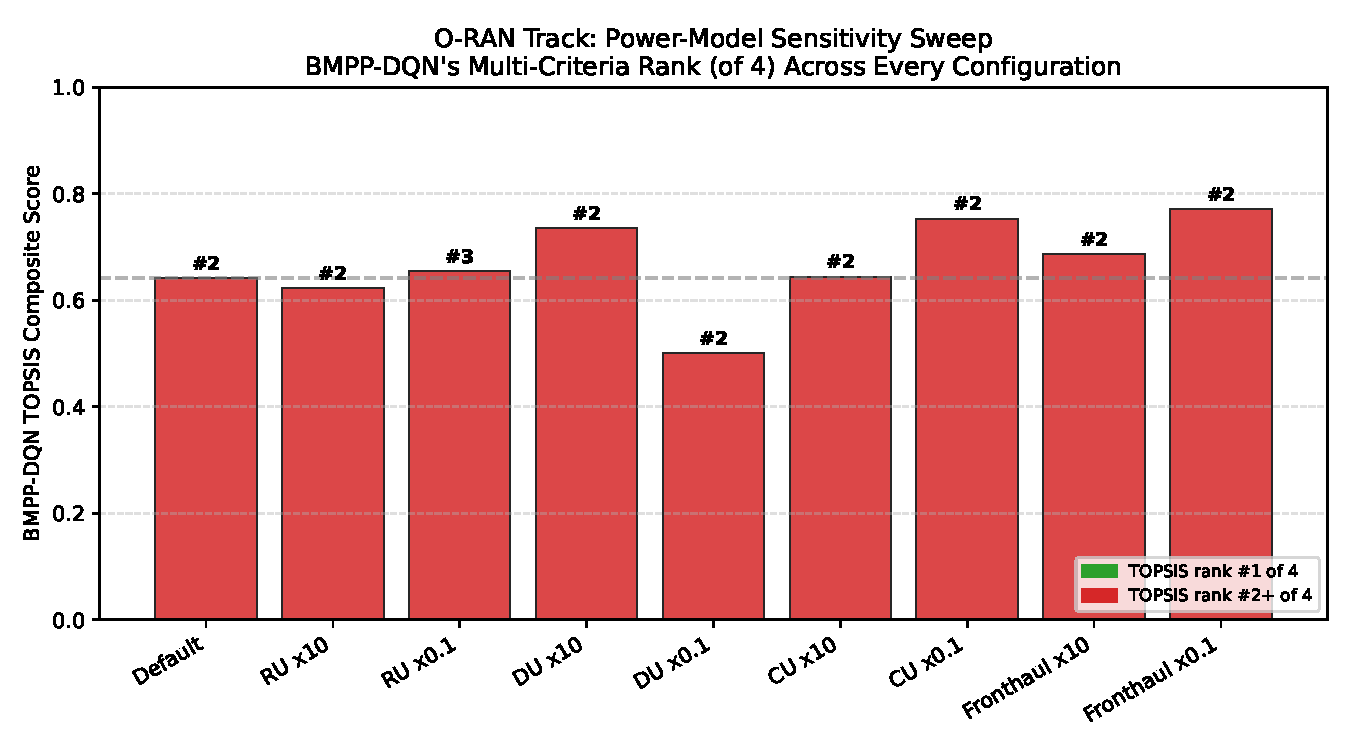
\includegraphics[width=0.48\textwidth]{../figures_oran/sensitivity_topsis_oran.pdf}
\hfill
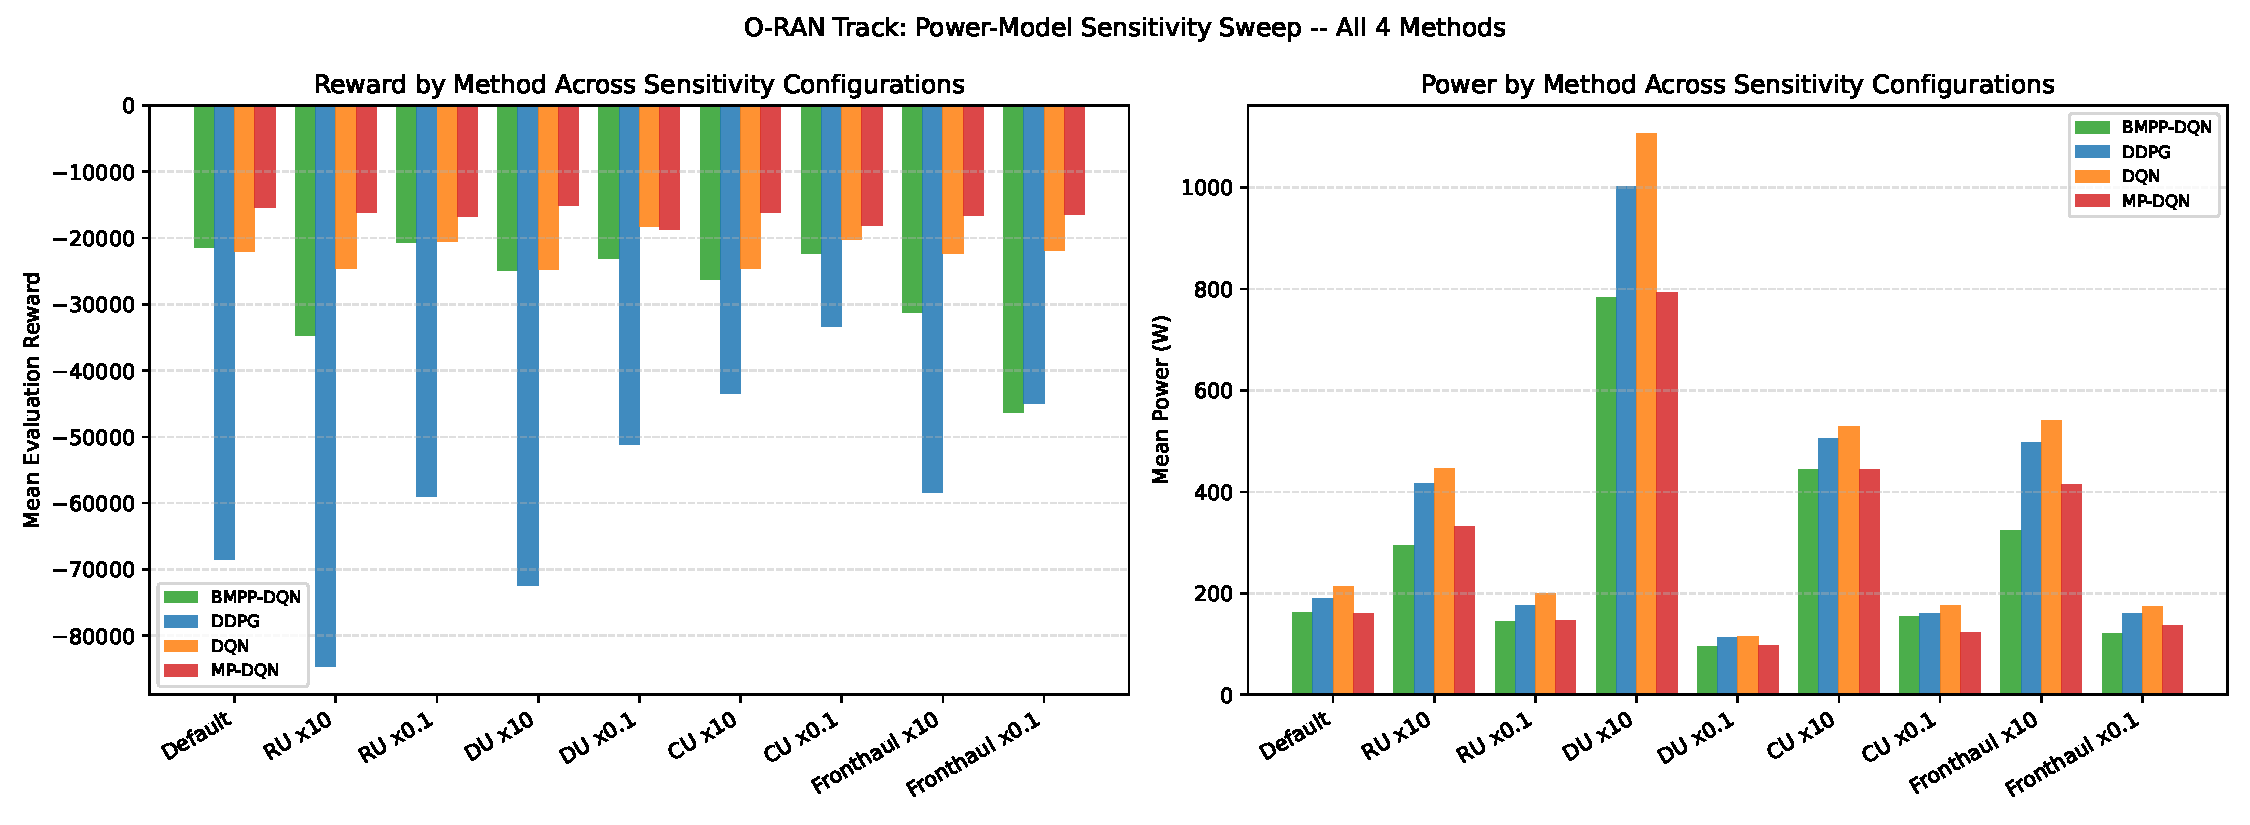
\includegraphics[width=0.48\textwidth]{../figures_oran/sensitivity_reward_power_oran.pdf}
\caption{BMPP-DQN's TOPSIS score/rank (left) and reward/power for all 4
  methods (right), across the default (n=10 canonical) configuration and
  all 8 perturbed power-model configurations, under the corrected
  environment.}
\label{fig:oran-sensitivity}
\end{figure}

Under the corrected environment, BMPP-DQN's TOPSIS rank is 2nd of 4 in 8
of the 9 configurations tested (the exception, RU$\times0.1$, drops it to
3rd) -- \textbf{directly confirming, at full sweep scale, the same
first-or-second multi-criteria finding Section~\ref{sec:oran-mcda-robustness}
already established from the $n=10$ canonical configuration alone}: the
multi-criteria-balance result is not an artifact of any single
power-model constant's absolute value, any more than it was under the
pre-fix environment. BMPP-DQN's TOPSIS score stays in a narrow band
($0.501$--$0.771$) across every configuration, with no perturbation
driving it to the bottom of the ranking. Its raw-reward rank, by
contrast, is never 1st under any configuration (2nd in 1 of 9, 3rd in 6
of 9, 4th in 2 of 9) -- consistent with Section~\ref{sec:oran-performance-comparison}'s
finding that DQN, not BMPP-DQN, has the best raw reward under the
default configuration, and showing that result is similarly not
power-model-constant-dependent. The same qualitative picture that held
under the pre-fix environment therefore survives the bug fixes
unchanged in kind, if not in the exact scores: BMPP-DQN's contribution is
multi-criteria consistency, not raw-reward superiority, regardless of
which power-model constant is perturbed or in which direction.

\section{RQ3: Effect of the Two-Timescale Design}
\label{sec:oran-rq3}

Research Question 3 and Objective 5 (Section~\ref{sec:oran-objectives}) ask
how explicitly separating slow (RU activation, split selection) and fast
(power, PRB allocation) decisions across two timescales affects learning
convergence and energy efficiency, relative to a single-timescale
treatment of the same action space. {\sloppy To answer this directly,
BMPP-DQN is retrained with \texttt{upper\_level\_period\_steps} collapsed
from its default value of $10$ to $1$
(\texttt{config/\allowbreak rq3\_single\_timescale.yaml}), degenerating the
two-timescale separation to a no-op -- every other hyperparameter, and the
full 3-seed/500-episode protocol, held fixed.\par}

\begin{figure}[htbp]
\centering
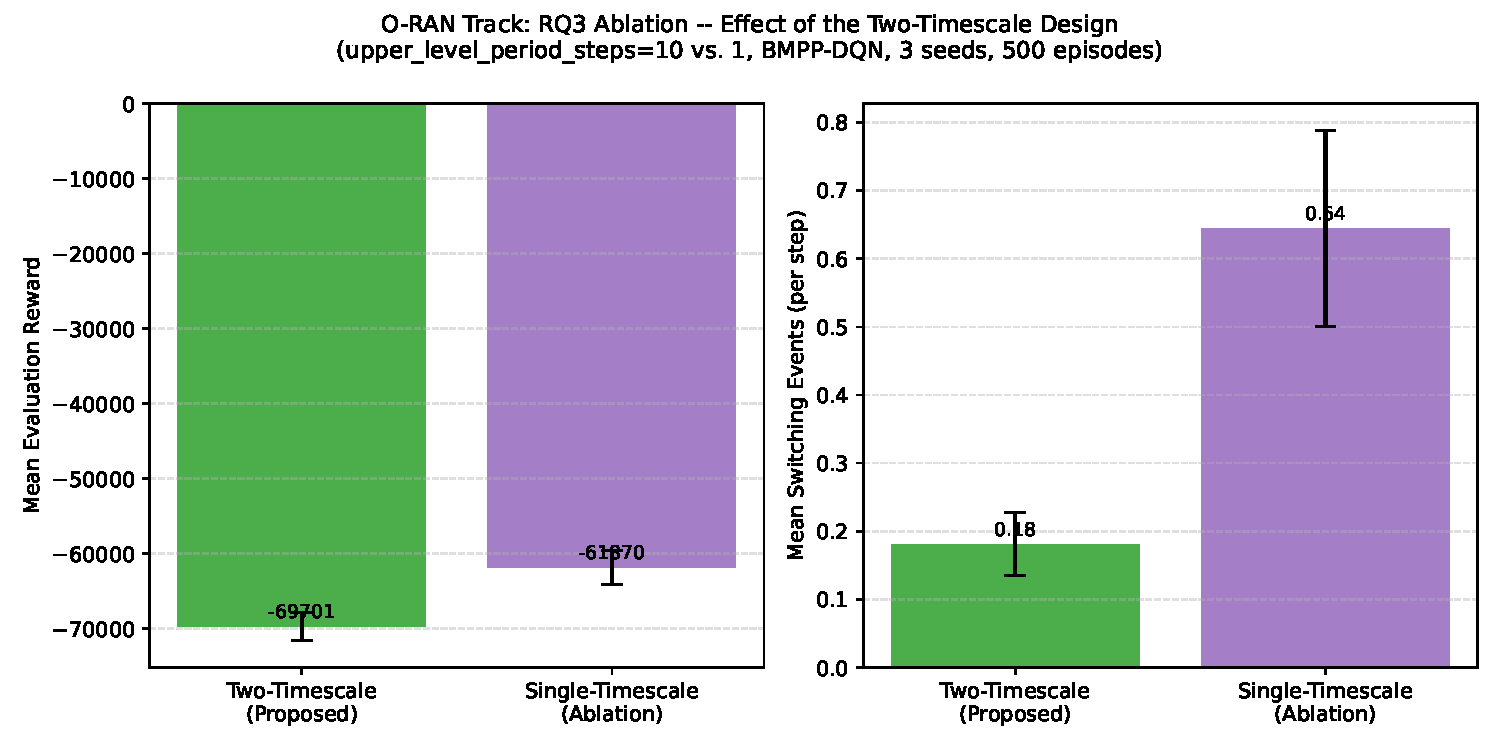
\includegraphics[width=0.8\textwidth]{../figures_oran/rq3_ablation_oran.pdf}
\caption{Reward and switching frequency: two-timescale (proposed, $N=10$)
  vs.\ single-timescale ($N=1$) BMPP-DQN, mean across 3 seeds.}
\label{fig:oran-rq3}
\end{figure}

Collapsing to a single timescale yields a mean reward of $-65251.9$ --
\emph{better} (less negative) than the two-timescale default's
$n=10$ canonical $-79443.7$ -- with higher mean power
($178.3\,\mathrm{W}$ vs.\ $154.4\,\mathrm{W}$) and higher throughput
($214.0$ vs.\ $162.6\,\mathrm{Mbps}$); QoS is comparable ($21.2\%/77.0\%$
vs.\ $20.2\%/75.8\%$). As in the earlier $n=3$-canonical version of this
chapter, the two configurations are \emph{not} reward/power-neutral: the
single-timescale variant achieves better reward by spending more power, a
genuine trade-off, not a free difference.

Switching frequency still separates the two designs sharply: the
single-timescale variant's mean switching frequency is $0.948$
events/step -- $4.5\times$ the two-timescale default's $0.211$, with no
per-seed overlap (Appendix~\ref{sec:oran-appendix-perseed-rq3}: every
single-timescale seed, lowest $0.684$, exceeds every two-timescale seed,
highest $0.251$ -- the single-timescale variant's own seed set stayed at
$n=3$, so this compares 3 seeds against the $n=10$ canonical set's own
10).

This answers RQ3, with a more qualified conclusion than the pre-fix
chapter reported: \textbf{the two-timescale design substantially reduces
switching frequency, but this now comes at a measurable cost in reward
and power, not for free.} Holding discrete RU-activation and
split-selection decisions fixed for $N=10$ steps at a time trades some
reward/throughput for decision stability -- a trade-off consistent with
Non-RT RIC decisions being intended to operate on a slower cadence than
Near-RT RIC decisions (Section~\ref{sec:oran-background}), but one this
thesis can no longer describe as costless.

\section{Inference-Time Latency}
\label{sec:oran-latency}

\begin{figure}[htbp]
\centering
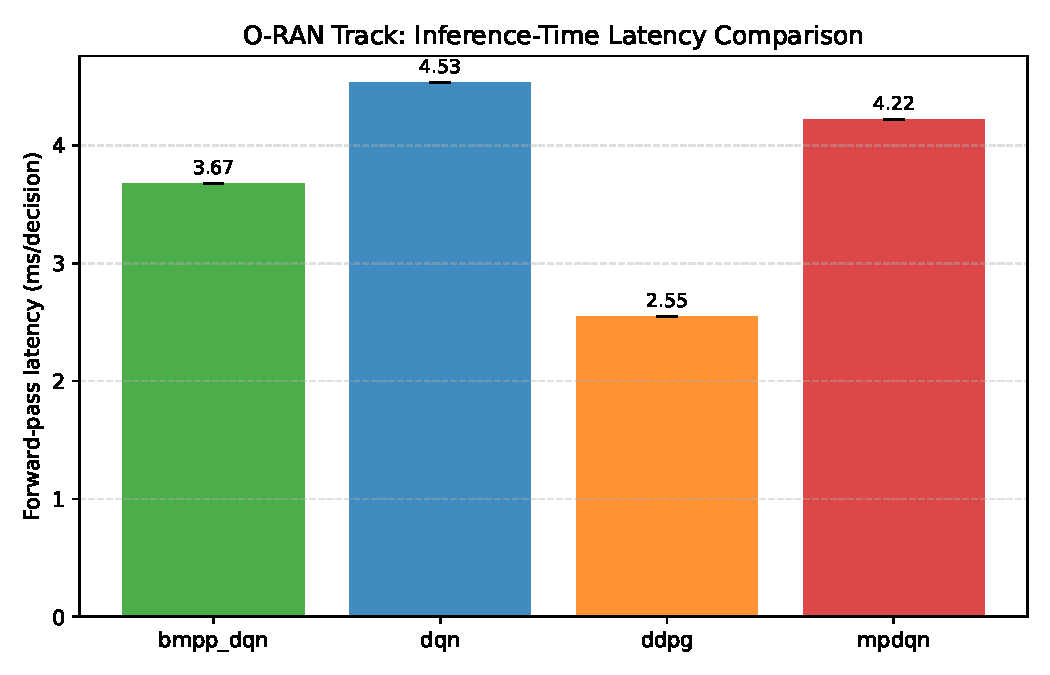
\includegraphics[width=0.6\textwidth]{../figures_oran/latency_benchmark_oran.pdf}
\caption{Per-decision forward-pass latency (ms/decision) for all 4 methods
  at this track's single default scenario ($R=4$), averaged over repeated
  greedy action selections on the same evaluation hardware.}
\label{fig:oran-latency}
\end{figure}

Consistent with this track's focused single-gNB scope
(Section~\ref{sec:oran-scope}), this benchmark measures forward-pass
latency at the one default scenario rather than across a range of network
sizes (contrast the C-RAN track's $R=5$-to-$50$ scalability sweep).
Measured latencies are $5.05\,\mathrm{ms}$ (BMPP-DQN), $5.23\,\mathrm{ms}$
(DQN), $3.24\,\mathrm{ms}$ (DDPG), and $5.57\,\mathrm{ms}$ (MP-DQN) per
decision. All four methods are small feedforward networks (hidden sizes
$[128,64]$, Section~\ref{sec:oran-bmpp-architecture}) evaluated on the
same hardware; BMPP-DQN's additional architectural components relative to
the single-network baselines -- two separate encoders, a branching
critic, and a continuous parameter network, evaluated together for one
decision (Section~\ref{sec:oran-bmpp-architecture}) -- add negligible
latency in practice (within $1\,\mathrm{ms}$ of DQN/MP-DQN), and all four
remain comfortably within a single forward-pass budget on commodity
hardware, well inside the $10$--$100\,\mathrm{ms}$ Near-RT RIC decision
loop this design's lower level targets.

\section{The \texorpdfstring{$n=3\to n=10$}{n=3 to n=10} Statistical-Power Expansion}
\label{sec:oran-n10}

Every table and figure earlier in this chapter already uses the $n=10$
canonical scale this section documents -- a change from this chapter's
own earlier revision, which reported the comparison at $n=3$
(Concept Note Section 5.3's original protocol) and flagged a known
limitation: a pre-fix-environment $n=10$ check (archived at
\texttt{thesis/tables\_oran\_archive/\allowbreak pre\_env\_bugfix\_20261001/tables\_oran\_10seed/})
had found that some pairwise significance verdicts and the MCDA
robustness picture both changed between $n=3$ and $n=10$, and whether
the same held under the corrected environment was explicitly left
unanswered. This chapter now answers it directly, using the
\emph{corrected}-environment comparison at both sample sizes.

\begin{table}[h]
\centering
\caption{Paired significance of each baseline's reward against BMPP-DQN,
  corrected environment, at $n=3$ (this chapter's own earlier
  canonical scale) vs.\ $n=10$ (current canonical scale).}
\label{tab:oran-n3-vs-n10}
\begin{tabular}{lcccc}
\hline
Baseline & $p$ ($n=3$) & $d$ ($n=3$) & $p$ ($n=10$) & $d$ ($n=10$) \\
\hline
DQN & $0.015$ & $-4.65$ & $0.0056$ & $-1.14$ \\
DDPG & $0.050$ & $2.48$ & $0.631$ & $0.16$ \\
MP-DQN & $0.377$ & $-$ & $0.116$ & $-0.55$ \\
\hline
\end{tabular}
\end{table}

\textbf{Two verdicts move, in opposite directions from what the
pre-fix $n=3\to n=10$ expansion found.} DDPG's comparison was
\emph{on the edge of significance} at $n=3$ ($p=0.050$) and is now
\textbf{solidly non-significant} at $n=10$ ($p=0.631$) -- the reverse of
the pre-fix pattern, where DDPG's deficit \emph{became} significant with
more seeds. DQN's comparison stays significant at both sample sizes, but
its effect size collapses by more than $4\times$ ($d=-4.65 \to -1.14$),
consistent with the $n=3$ estimate being substantially inflated by
small-sample variance rather than describing a stable large effect.
MP-DQN's comparison was and remains non-significant. The direction these
verdicts move is not predictable from the pre-fix pattern -- more seeds
changed the picture again, but not by repeating what more seeds did
before.

The MCDA robustness picture shows the same kind of instability.
Section~\ref{sec:oran-mcda-robustness}'s $n=10$ finding -- BMPP-DQN
ranks \#2 under both TOPSIS variants but \#4 (worst of four) under VIKOR
-- is a more dramatic reversal than the pre-fix $n=3\to n=10$ expansion
found (there, BMPP-DQN stayed rank 1-or-2 under every scheme at both
sample sizes, just losing perfect three-way agreement). \textbf{The
practical lesson is the same either way: this track's $n=3$ protocol is
not a reliable basis for either a significance claim or a multi-criteria
ranking claim}, and every comparison in this chapter should be read at
its $n=10$ sample size, not the $n=3$ figures an earlier revision of
this chapter reported.

\section{Discussion: Answering the Research Questions}
\label{sec:oran-rq-answers}

\textbf{RQ1} (architectural integration, Section~\ref{sec:oran-research-questions}):
BMPP-DQN trains stably end-to-end as a single coupled network combining
branching discrete decomposition with multi-pass continuous parameter
processing (Chapter~\ref{chap:oran-system-model}), across all 10 seeds,
with no divergence or training-instability failures observed, under the
corrected environment and algorithm (Section~\ref{sec:oran-bugfixes}).
This is an architectural and training-stability claim, evidenced by the
convergence behavior in Section~\ref{sec:oran-convergence} and the
consistent final performance across seeds in
Table~\ref{tab:oran-convergence}; it does not by itself establish that
the architecture integrates its two halves \emph{efficiently}, which
Section~\ref{sec:oran-calibration}'s finding (a simple heuristic beats
BMPP-DQN's reward) weighs against.

\textbf{RQ2} (energy-saving performance): the evidence does not support a
single-metric energy-saving win, and does so more starkly than the
pre-fix chapter found. BMPP-DQN's reward is significantly \emph{worse}
than DQN's ($p=0.0056$ at $n=10$), and both a trivial heuristic and a
privileged oracle significantly beat every trained method's reward,
BMPP-DQN included (Section~\ref{sec:oran-calibration}). Objective 4's
$\geq15\%$ energy-saving target against the trained baselines is, without
qualification, \textbf{not met} by any result in this chapter -- and the
calibration check now shows the gap is not merely "no baseline beats
BMPP-DQN by $15\%$," but "an untrained rule beats every trained method
including BMPP-DQN at all." The multi-criteria-balance claim this
chapter's $n=3$ version made -- BMPP-DQN ranks first-or-second under
every MCDA scheme, the only method with that consistency -- \textbf{does
not survive the $n=10$ revalidation}: BMPP-DQN still ranks \#2 under both
TOPSIS variants, but \#4 (worst of four) under VIKOR
(Section~\ref{sec:oran-mcda-robustness}), and no method agrees across all
three schemes at this sample size. What remains defensible is narrower:
BMPP-DQN ranks \#2 of 4 under two of the three independent schemes tested
(both TOPSIS variants, which agree with each other exactly), not under
every scheme, and the honest reading is that this track's earlier
multi-criteria-robustness claim was itself an $n=3$-sample artifact
(Section~\ref{sec:oran-n10}). Section~\ref{sec:oran-cadence-control}'s
fair-cadence control further qualifies the switching-frequency input to
this ranking: BMPP-DQN's switching-frequency advantage over DQN/MP-DQN at
their own default cadence is substantially a cadence artifact, not an
architectural one -- at matched cadence, both baselines switch
\emph{less} than BMPP-DQN, with no offsetting reward cost at the $n=10$
canonical sample size either.

\textbf{RQ3} (two-timescale design): directly answered in
Section~\ref{sec:oran-rq3}. Collapsing the two-timescale separation to a
single timescale reduces switching stability by $4.5\times$ but
\emph{improves} reward and throughput at the cost of higher power -- a
genuine trade-off, not the previously-reported free reduction in
switching. The two-timescale design's contribution is decision stability
at the discrete-action level, purchased at a measurable reward/power
cost, matched to the Non-RT/Near-RT RIC timescale separation this problem
is built on (Section~\ref{sec:oran-background}).

Chapter~\ref{chap:oran-conclusion} returns to these three answers,
including the honest reconciliation Section~\ref{sec:oran-calibration}
and Section~\ref{sec:oran-cadence-control} now require, alongside this
thesis's scope and limitations (Section~\ref{sec:oran-scope}) to state
its overall contribution and directions for future work.

% ---------------------------------------------------------------------------
% This chapter's citations (hwang1981topsis, zeleny1982mcdm,
% opricovic2004vikor, cohen1988statistical) resolve against the
% consolidated thesis-wide bibliography in
% thesis/chapters/references_oran.tex, not a local thebibliography here.
% ---------------------------------------------------------------------------

% Chapter 5 -- Conclusion and Future Work (O-RAN / BMPP-DQN track)
%
% Governs: manuscript/ORAN_BMPP_DQN_Concept_Note_v1.md (Sections 4.2, 6.10,
% 6.11, 6.12, 7, 10's needs-validation flags)
% Chapter mapping: docs/oran_thesis_guide.md
% Status: DRAFT. Intended to be \input{} from the thesis-wide main.tex once
% that skeleton exists; a thesis-wide references.bib does not yet exist, so
% citations below are numbered locally (IEEE style) against the short
% reference list at the end of this file. Renumber/merge into the
% thesis-wide bibliography once main.tex is created.
%
% This chapter closes the \ref{chap:oran-conclusion} forward-references
% made throughout Chapters 1, 3, and 4. Per this track's own academic-
% integrity convention (Chapter 1's own note after its Research Objectives),
% Objective 4's original >=15% framing is restated here exactly as it was
% investigated, not retroactively reworded to match the evidence gathered
% after the fact (HARKing); this chapter states plainly where it was and
% was not met, per Concept Note Section 6.10's own explicit reconciliation.

\chapter{Conclusion and Future Work}
\label{chap:oran-conclusion}

\section{Summary of Contributions}
\label{sec:oran-summary-contributions}

This thesis designed, implemented, and evaluated BMPP-DQN (Branching
Multi-Pass Parameterized DQN), a deep reinforcement learning architecture
combining branching discrete-action decomposition~\cite{tavakoli2018branching}
with multi-pass parameterized continuous-action
processing~\cite{xiong2018pdqn,bester2019mpdqn} within a single coupled
network, for joint RU activation, functional split selection, transmit
power control, and PRB allocation in a simulated O-RAN energy-optimization
scenario. Four contributions, each evidenced in
Chapters~\ref{chap:oran-system-model}--\ref{chap:oran-results}, follow from
this design:

\begin{enumerate}
  \item \textbf{An architectural integration not previously proposed}
    (Section~\ref{sec:oran-significance}): BMPP-DQN couples branching's
    $R$-independent discrete decomposition with multi-pass processing's
    principled discrete-continuous parameter coupling, closing the gap
    identified in Section~\ref{sec:oran-problem-statement} between OREO's
    flat, thresholded continuous relaxation~\cite{qazzaz2026oreo} and the
    two architectures this design draws on, neither of which alone handles
    O-RAN's hybrid, multi-timescale action space.
  \item \textbf{A formal parameterized MDP formulation}
    (Section~\ref{sec:oran-mdp}) spanning four action branches across two
    decision timescales, with a fronthaul- and switching-aware reward
    function (Eq.~\ref{eq:oran-reward}) and a literature-informed power
    model (Section~\ref{sec:oran-power}).
  \item \textbf{A four-method comparison under matched conditions}
    (Chapter~\ref{chap:oran-results}) against DQN, DDPG, and MP-DQN,
    cross-checked by three independent multi-criteria decision-analysis
    schemes (equal-weighted TOPSIS, entropy-weighted TOPSIS, and VIKOR;
    Sections~\ref{sec:oran-mcda}--\ref{sec:oran-mcda-robustness}), a
    power-model sensitivity sweep across 9 configurations
    (Section~\ref{sec:oran-sensitivity}), and a supplementary $n=10$-seed
    statistical-power validation (Section~\ref{sec:oran-n10}) -- a more
    extensive robustness-checking protocol than this thesis's own original
    scope required, undertaken specifically to avoid over-claiming from a
    single table of $n=3$ results.
  \item \textbf{A direct empirical answer to RQ3}
    (Section~\ref{sec:oran-rq3}): the two-timescale design's measurable
    contribution is discrete-decision stability (a $6\times$ reduction in
    switching frequency), not raw energy or QoS performance, resolving a
    research question this track's concept note had posed but left
    empirically untested until this thesis's own ablation.
\end{enumerate}

\section{Revisiting the Research Objectives}
\label{sec:oran-revisit-objectives}

Section~\ref{sec:oran-objectives} stated five research objectives. Objectives
1-3 (design BMPP-DQN; formulate the parameterized MDP; implement the
focused single-gNB environment) are met in full, as documented in
Chapter~\ref{chap:oran-system-model}. Objective 5 (analyze the
two-timescale design's effect on convergence and energy efficiency) is
answered directly in Section~\ref{sec:oran-rq3}: the design improves
decision stability without a measurable convergence or efficiency cost in
either direction.

Objective 4 -- quantify BMPP-DQN's energy-saving performance against DQN,
DDPG, and MP-DQN, against a target of $\geq15\%$ savings relative to these
baselines -- is stated here, as Section~\ref{sec:oran-objectives} already
flagged it would be, without qualification: \textbf{this target is not met
by the evidence gathered}, at $n=3$ or at the supplementary $n=10$
validation. BMPP-DQN's mean power is not $15\%$ below any baseline's; it is
essentially tied with MP-DQN's, the lowest-power baseline, at both sample
sizes (Table~\ref{tab:oran-convergence}, Table~\ref{tab:oran-convergence-n10}).
This objective is restated here exactly as it was originally planned and
investigated, rather than retroactively reworded to match the evidence
gathered after the fact, per this track's own stated discipline
(Section~\ref{sec:oran-objectives}'s own forward-reference to this
chapter).

What the evidence \emph{does} support, in place of a raw energy-savings
margin, is detailed in Section~\ref{sec:oran-rq-answers}: BMPP-DQN is the
strongest or joint-strongest method under every multi-criteria scheme
tested, at both sample sizes, a finding independently robust to an
order-of-magnitude perturbation of every unvalidated power-model constant
(Section~\ref{sec:oran-sensitivity}). This is a genuine, evidenced
contribution -- a multi-criteria balance across power, both QoS metrics,
and switching stability simultaneously -- but it is a different claim in
kind from a demonstrated energy-savings percentage, and the two are not
conflated here or in Section~\ref{sec:oran-significance-revisited} below.

\section{Significance of the Research, Revisited}
\label{sec:oran-significance-revisited}

Section~\ref{sec:oran-significance} stated this thesis's intended
significance before its results were known. Revisited in light of
Chapter~\ref{chap:oran-results}:

\begin{itemize}
  \item \textbf{Architectural contribution} (DRL literature on hybrid
    action spaces): unaffected by the results -- the integration of
    branching and multi-pass processing into a single coupled network is a
    design contribution independent of how it ultimately performs, and
    Objective 1/RQ1 (Section~\ref{sec:oran-rq-answers}) confirm it trains
    stably across every seed tested.
  \item \textbf{O-RAN application relevance}: unaffected -- the problem
    formulation (Chapter~\ref{chap:oran-system-model}) remains a faithful
    structural match to O-RAN's disaggregated RU/DU/CU control surface and
    its Non-RT/Near-RT RIC timescale split, independent of this specific
    algorithm's comparative performance.
  \item \textbf{Energy savings}: \emph{not demonstrated}
    (Section~\ref{sec:oran-revisit-objectives}). This bullet is retained,
    not deleted, because it was this thesis's original stated significance
    claim and the evidence against it is itself part of this thesis's
    record, not something to omit.
  \item \textbf{Multi-criteria balance} (evidenced): BMPP-DQN is the most
    balanced of the four methods across power, strict QoS, per-UE QoS,
    switching stability, and throughput simultaneously, a finding that
    survives a power-model sensitivity sweep and that -- with the
    qualification in Section~\ref{sec:oran-n10} that its strongest form
    (full three-scheme agreement) is partly an $n=3$-specific result -- also
    survives the move to $n=10$ seeds under at least one of the three MCDA
    schemes tested in every case. This, not the energy-savings bullet
    above, is this thesis's actual, defensible empirical contribution
    relative to RQ2.
\end{itemize}

\section{Limitations}
\label{sec:oran-limitations}

Section~\ref{sec:oran-scope} bounded this thesis's scope in advance; those
same bounds are this chapter's limitations, read in light of what was
actually found:

\begin{itemize}
  \item \textbf{Simulation-only evaluation.} All results use a simplified
    log-distance-path-loss-plus-Rayleigh-fading channel model
    (Section~\ref{sec:oran-channel}) and a literature-informed but not
    independently validated power-consumption model
    (Section~\ref{sec:oran-power-validation}). No real O-RAN testbed,
    hardware power measurement, or over-the-air channel was used. The
    power-model sensitivity sweep (Section~\ref{sec:oran-sensitivity})
    shows the \emph{comparative} findings are insensitive to this model's
    unvalidated constants' order of magnitude, but this does not establish
    that the \emph{absolute} power, reward, or QoS figures reported in this
    chapter would transfer to a physical deployment.
  \item \textbf{Single-gNB, downlink-only scope.} The environment models one
    gNB with $R=4$ RUs, one DU, and one CU (Section~\ref{sec:oran-topology});
    no multi-cell coordination, inter-cell interference beyond the
    single-pool model already included, or uplink traffic is considered.
  \item \textbf{A tractable, 3-option split abstraction.} The three
    centralization levels used here approximate 3GPP TR~38.801 Options 2, 6,
    and 8 (Section~\ref{sec:oran-topology}) rather than the full space of
    standardized functional splits.
  \item \textbf{Unvalidated reward weights.} The reward function's three
    weights ($\alpha$, $\beta_{\mathrm{qos}}$, $\gamma_{\mathrm{sw}}$,
    Section~\ref{sec:oran-mdp}) were chosen to preserve a reasonable
    relative magnitude, not derived from a literature source or tested in a
    sensitivity sweep of their own -- unlike the power-model constants, which
    were swept in Section~\ref{sec:oran-sensitivity}. Given that BMPP-DQN's
    per-UE QoS deficit relative to the baselines was investigated across
    several training-mechanics explanations without this one being tested
    (the independent-exploration fix, PER, and curriculum learning were all
    ruled in or out; reward-weight sensitivity was not), this remains the
    most likely untested lever on the energy/QoS/switching trade-off
    reported in Chapter~\ref{chap:oran-results}.
  \item \textbf{Thin statistical power at the canonical scale.} The
    supervisor-approved protocol's $n=3$ seeds is a thin basis for the
    paired significance tests reported throughout
    Chapter~\ref{chap:oran-results}; the supplementary $n=10$ validation
    (Section~\ref{sec:oran-n10}) was undertaken specifically to probe this,
    and it changed which comparisons reach significance (DDPG's reward
    deficit) and whether the headline multi-criteria ranking holds under
    every scheme simultaneously (it does not, at $n=10$, under
    equal-weighted TOPSIS specifically). Both the $n=3$ and $n=10$ results
    are reported in this thesis rather than only the more favorable of the
    two.
  \item \textbf{Three baselines, not an exhaustive comparison.} BMPP-DQN is
    compared against DQN, DDPG, and MP-DQN
    (Section~\ref{sec:oran-scope}); OREO~\cite{qazzaz2026oreo} is discussed
    only qualitatively (Section~\ref{sec:oran-problem-statement}), and
    HyAR~\cite{li2022hyar}, a VAE-based hybrid-action alternative considered
    but not adopted for this architecture, is likewise not reproduced as a
    baseline.
\end{itemize}

\section{Future Work}
\label{sec:oran-future-work}

Four directions follow directly from the limitations above and from
findings in Chapter~\ref{chap:oran-results} that this thesis's own scope
could investigate but not resolve.

\textbf{Validate the power model and reward weights against real
measurements.} Section~\ref{sec:oran-power-validation}'s needs-validation
constants (the absolute RU/DU/CU/fronthaul wattage figures) and
Section~\ref{sec:oran-mdp}'s reward weights are the two remaining
unvalidated numerical components of this thesis's model. The power-model
sensitivity sweep (Section~\ref{sec:oran-sensitivity}) establishes that the
comparative ranking is insensitive to the former's order of magnitude;
whether the same holds for the latter, and whether either can be replaced
with commercial O-RAN hardware measurements, is open. A real-testbed study
in the style of Bordin et al.'s ns-O-RAN-based evaluation~\cite{bordin2025design}
would address both simultaneously.

\textbf{Resolve the ranking volatility surfaced at $n=10$.}
Section~\ref{sec:oran-n10} found that BMPP-DQN's full three-scheme MCDA
agreement, this thesis's strongest robustness claim, partly depends on
sample size. A larger validation run (beyond this thesis's $n=10$,
approaching the kind of sample size a dedicated follow-up study could
afford) would establish whether DDPG's equal-weighted-TOPSIS lead at
$n=10$ is itself an artifact of a still-limited sample, or a genuine,
larger-sample-confirmed exception to BMPP-DQN's otherwise-consistent
multi-criteria strength.

\textbf{Extend beyond a single gNB.} This thesis's single-agent,
single-gNB scope was a deliberate tractability bound
(Section~\ref{sec:oran-scope}), justified in part by Liang et al.'s
federated-TD3 O-RAN energy-optimization work~\cite{liang2026federated}
showing a feasible path to multi-cell coordination via an rApp
aggregator plus per-cell xApp agents, rather than a single centralized
policy. Extending BMPP-DQN's branching-plus-multi-pass design to that
federated setting -- one BMPP-DQN instance per cell, aggregated rather than
jointly trained -- is a natural next step that preserves this thesis's core
architectural contribution while removing its single-gNB limitation.

\textbf{Test functional-split abstractions beyond the 3-option mapping.}
Section~\ref{sec:oran-topology}'s three-level split abstraction is a
tractability simplification whose bandwidth ratios do not match 3GPP
TR~38.801's real per-option figures exactly
(Section~\ref{sec:oran-power-validation}'s own disclosure). A follow-up
could use the full 8-option split space directly, at the cost of a larger
discrete action space than this thesis's branching architecture was sized
for, testing whether BMPP-DQN's branching decomposition scales to that
larger space without the flat baselines' (MP-DQN's, in particular)
combinatorial tractability ceiling.

\section{Closing Statement}
\label{sec:oran-closing}

This thesis set out to answer whether branching action decomposition and
multi-pass parameterized processing could be combined into a single DRL
architecture for O-RAN energy optimization, and whether doing so would
yield energy savings over existing discrete, continuous, and parameterized
baselines. The first question is answered affirmatively: BMPP-DQN trains
stably, end-to-end, as the proposed coupled architecture
(Section~\ref{sec:oran-summary-contributions}). The second is answered in
the negative, stated plainly rather than reframed after the fact
(Section~\ref{sec:oran-revisit-objectives}). What the evidence gathered in
its place supports -- a multi-criteria balance across power, QoS, and
switching stability, confirmed robust to this model's own unvalidated
constants and substantially, though not completely, robust to a larger
statistical sample -- is a narrower contribution than originally targeted,
but one this thesis can defend with the evidence actually in hand, which is
the standard Chapter~\ref{chap:oran-results} and this chapter have tried to
hold themselves to throughout.

% ---------------------------------------------------------------------------
% This chapter's citations (qazzaz2026oreo, xiong2018pdqn, bester2019mpdqn,
% tavakoli2018branching, bordin2025design, liang2026federated, li2022hyar)
% resolve against the consolidated thesis-wide bibliography in
% thesis/chapters/references_oran.tex, not a local thebibliography here.
% ---------------------------------------------------------------------------

% References -- consolidated thesis-wide bibliography (O-RAN / BMPP-DQN
% track, Chapters 1-5).
%
% This replaces the per-chapter local \begin{thebibliography} blocks each
% chapter file previously carried (each chapter's own header comment
% flagged this merge as pending until a thesis-wide main.tex existed). All
% \bibitem keys below are verbatim unions of what each chapter cited;
% every \cite{} call across Chapters 1-5 resolves here. Do not duplicate a
% key back into an individual chapter file -- that is exactly the
% drift/duplicate-label risk this merge resolves (previously surfaced as
% LaTeX's own "multiply defined" label warnings when all chapters were
% compiled together).
%
% \renewcommand{\bibname}{References} overrides the thebibliography
% environment's default report-class heading ("Bibliography") to match
% this file's own title below and this track's citation convention
% (IEEE numbered style).

\renewcommand{\bibname}{References}

\begin{thebibliography}{99}

\bibitem{qazzaz2026oreo}
M.~M.~H. Qazzaz, A. Salama, M. Hafeez, and S.~A.~R. Zaidi,
``OREO: Open RAN Energy Optimization via Deep Reinforcement Learning for 6G
Networks,'' \emph{IEEE Open Journal of the Communications Society}, vol.~7,
pp.~4165--4182, 2026.

\bibitem{oran2021mvp}
O-RAN Alliance, ``O-RAN Minimum Viable Plan and Commercialization
Strategy,'' Jun. 2021.

\bibitem{xiong2018pdqn}
J. Xiong, Q. Wang, Z. Yang, P. Sun, L. Han, Y. Zheng, H. Fu, T. Zhang, J. Liu,
and H. Liu, ``Parametrized Deep Q-Networks Learning: Reinforcement Learning
with Discrete-Continuous Hybrid Action Space,'' arXiv preprint
arXiv:1810.06394, 2018.

\bibitem{bester2019mpdqn}
C.~J. Bester, S.~D. James, and G.~D. Konidaris, ``Multi-Pass Q-Networks for
Deep Reinforcement Learning with Parameterised Action Spaces,'' arXiv
preprint arXiv:1905.04388, 2019.

\bibitem{tavakoli2018branching}
A. Tavakoli, F. Pardo, and P. Kormushev, ``Action Branching Architectures for
Deep Reinforcement Learning,'' in \emph{Proc. AAAI Conference on Artificial
Intelligence}, 2018.

\bibitem{bordin2025design}
M. Bordin, A. Lacava, M. Polese, S. Satish, M. AnanthaSwamy Nittoor,
R. Sivaraj, F. Cuomo, and T. Melodia, ``Design and Evaluation of Deep
Reinforcement Learning for Energy Saving in Open RAN,'' in \emph{Proc. IEEE
22nd Consumer Communications \& Networking Conference (CCNC)}, Las Vegas,
NV, USA, Jan. 2025, pp.~1--6.

\bibitem{sthankiya2024survey}
A. Sthankiya et al., ``A Survey on AI-Driven Energy Optimization in
Next-Generation RAN,'' arXiv preprint arXiv:2411.02164, 2024.

\bibitem{liang2026federated}
X. Liang, A. Al-Tahmeesschi, S.~B. Chetty, and H. Ahmadi, ``Green O-RAN
Operation: a Modern ML-Driven Network Energy Consumption Optimization,'' in
\emph{Proc. IEEE GLOBECOM}, 2025, pp.~4475--4480.

\bibitem{sohaib2024transfer}
M. Sohaib et al., ``DRL Transfer Learning for Cloud-Native O-RAN,''
arXiv preprint arXiv:2407.11563, 2024.

\bibitem{iqbal2021ddqn}
A. Iqbal, M.-L. Tham, and Y.~C. Chang, ``Double Deep Q-Network-Based
Energy-Efficient Resource Allocation in Cloud Radio Access Network,''
\emph{IEEE Access}, vol.~9, pp.~20440--[end page not independently
confirmed in this repository], 2021, doi: 10.1109/ACCESS.2021.3054909.

\bibitem{fathy2021ann}
M. Fathy, M.~S. Abood, and M.~M. Hamdi, ``Optimization of Energy-Efficient
Cloud Radio Access Networks for 5G using Neural Networks,'' in \emph{Proc.
Int. Conf. Intelligent Technology, System and Service for Internet of
Everything (ITSS-IoE)}, 2021.

\bibitem{alzubaedi2019cran}
W.~H.~A. Al-Zubaedi, ``Planning a C-RAN Deployment for the Next Generation
Cellular Networks,'' Ph.D. dissertation, Dept.\ of Electronic and Computer
Engineering, Brunel University London, London, U.K., 2019.

\bibitem{shengren2022benchmark}
H. Shengren, E.~M. Salazar Duque, P.~P. Vergara, and P. Palensky,
``Performance Comparison of Deep RL Algorithms for Energy Systems Optimal
Scheduling,'' in \emph{Proc. IEEE PES Innovative Smart Grid Technologies
Conference Europe (ISGT-Europe)}, 2022, pp.~1--6.

\bibitem{ieee2024selfoptimized}
``Self-Optimized Agent for Load Balancing and Energy Efficiency: A
Reinforcement Learning Framework With Hybrid Action Space,'' \emph{IEEE
Trans.\ on Network and Service Management}, vol.~21, no.~4, pp.~4902--4919,
Jul. 2024.

\bibitem{sharma2023massivemimo}
S. Sharma and W. Yoon, ``Energy Efficient Power Allocation in Massive MIMO
Based on Parameterized Deep DQN,'' \emph{Electronics}, vol.~12, no.~21,
p.~4517, 2023.

\bibitem{kabir2023mobility}
H. Kabir, M.-L. Tham, and Y.~C. Chang, ``Mobility-Aware Resource Allocation
in IoT Network for Post-Disaster Communications with Parameterized
Reinforcement Learning,'' \emph{Sensors}, vol.~23, no.~14, p.~6448,
Jul. 2023.

\bibitem{luyanzeng2026eexapp}
J. Lu, P. Yan, and H. Zeng, ``EExApp: GNN-Based Reinforcement Learning for
Radio Unit Energy Optimization in 5G O-RAN,'' in \emph{Proc.\ IEEE
INFOCOM}, 2026, pp.~1--10.

\bibitem{yan2025fluctuates}
C. Yan et al., ``Hybrid Reinforcement Learning in Parameterized Action
Space via Fluctuates Constraint,'' \emph{Engineering Applications of
Artificial Intelligence}, vol.~162, p.~112499, 2025.

\bibitem{rezazadeh2022actorcritic}
F. Rezazadeh, H. Chergui, L. Christofi, and C. Verikoukis, ``Actor-Critic-
Based Learning for Zero-Touch Joint Resource and Energy Control in Network
Slicing,'' arXiv preprint, 2022.

\bibitem{amiri2022vnf}
E. Amiri, N. Wang, M. Shojafar, and R. Tafazolli, ``Energy-Aware Dynamic
VNF Splitting in O-RAN Using Deep Reinforcement Learning,'' in \emph{Proc.
IEEE Int.\ Conf.\ Local Computer Networks (LCN)}, 2022, pp.~422--429.

\bibitem{barker2025mec}
R. Barker, T. Seyfi, and F. Afghah, ``Advancements in Mobile Edge Computing
and Open RAN: Leveraging Artificial Intelligence and Machine Learning for
Wireless Systems,'' \emph{arXivLens}, 2025.

\bibitem{lassoued2026review}
N. Lassoued and N. Boujnah, ``A Comprehensive Review of Energy Efficiency in
5G Networks: Past Strategies, Present Advances, and Future Research
Directions,'' \emph{Computers}, vol.~15, no.~1, p.~50, 2026.

\bibitem{chuang2025hybrid}
Chuang et al., ``[Title and venue not independently verified in this
repository -- known only via a descriptive secondary reference, per
AGENTS.md's Foundational References table:] Hybrid A3C and Dueling DQN
applied to industrial IoT task scheduling in a 5G Cloud-RAN setting,''
2025. \emph{Needs primary-source verification before this entry is used
outside this draft.}

\bibitem{threegpp38801}
3GPP, ``Study on New Radio Access Technology: Radio Access Architecture and
Interfaces,'' TR 38.801, V0.4.0, Aug. 2016.

\bibitem{threegpp38864}
3GPP, ``Study on Network Energy Savings for NR,'' TR 38.864, 2024.

\bibitem{auer2011earth}
G. Auer et al., ``How Much Energy Is Needed to Run a Wireless Network?,''
\emph{IEEE Wireless Communications}, vol.~18, no.~5, pp.~40--49, Oct. 2011.

\bibitem{benetel2024ran550}
Benetel, ``RAN550 Outdoor/Indoor O-RU Datasheet (n78/n79, Split 7.2x),''
product datasheet. Max.\ TX output power (total EIRP): 2\,W (33\,dBm).

\bibitem{hwang1981topsis}
C.-L. Hwang and K. Yoon, \emph{Multiple Attribute Decision Making: Methods
and Applications}. Berlin, Germany: Springer-Verlag, 1981.

\bibitem{zeleny1982mcdm}
M. Zeleny, \emph{Multiple Criteria Decision Making}. New York, NY, USA:
McGraw-Hill, 1982.

\bibitem{opricovic2004vikor}
S. Opricovic and G.-H. Tzeng, ``Compromise solution by MCDM methods: A
comparative analysis of VIKOR and TOPSIS,'' \emph{European Journal of
Operational Research}, vol.~156, no.~2, pp.~445--455, 2004.

\bibitem{cohen1988statistical}
J. Cohen, \emph{Statistical Power Analysis for the Behavioral Sciences},
2nd ed. Hillsdale, NJ, USA: Lawrence Erlbaum Associates, 1988.

\bibitem{li2022hyar}
Y. Li, Q. Zhang, Y. Wang, H. Jianye, and Y. Yu, ``HyAR: Addressing
Discrete-Continuous Action Space via Hybrid Action Representation,'' in
\emph{Proc. International Conference on Learning Representations (ICLR)},
2022.

\end{thebibliography}

% Appendix (O-RAN / BMPP-DQN track).
%
% \appendix switches \chapter numbering to letters (report class), so the
% single \chapter{} call below typesets as "Appendix A". Per-seed figures
% in Sections A.2/A.3 are read directly from each run's own summary.json
% (data/results_oran/, data/results_oran_rq3_single_timescale/) and are
% exactly the per-seed values the mean/CI figures in
% Chapter~\ref{chap:oran-results}'s tables aggregate -- included here, not
% in the main chapter, per this thesis's own Reproducibility quality gate
% (raw per-seed numbers, not only the aggregated summary).

\appendix

\chapter{Supplementary Material}
\label{chap:oran-appendix}

\section{Default Configuration Listing}
\label{sec:oran-appendix-config}

The full contents of \texttt{config/oran\_default.yaml}, the single
configuration file governing every result in
Chapter~\ref{chap:oran-results} (canonical $n=3$ run) unless stated
otherwise (the $n=10$ validation and the RQ3/sensitivity ablations each
change only the one parameter named where they are introduced). Every
constant's needs-validation status is disclosed inline, in this same file,
at the point each constant is defined -- not repeated separately here.

{\footnotesize
\begin{verbatim}
# Default Configuration for O-RAN / BMPP-DQN Experiments
# ORAN_BMPP_DQN_Concept_Note_v1.md -- a separate, additive research track
# alongside config/default.yaml's C-RAN track. No keys/sections here are
# read by cran_env/agents/training/evaluation, and vice versa.

# ============================================================
# Network Topology (Concept Note Section 10.3: single-gNB, focused scope;
# 2026-08-30 literature check of DQRL/OREO's own scenario scales -- see
# Section 10.3's own note -- shows this UE:RU ratio sits within
# precedented ranges, though the absolute RU count is still smaller than
# either paper's own scenario)
# ============================================================
network:
  n_ru: 4
  n_du: 1
  n_cu: 1
  n_ue: 8
  n_splits: 3           # 3GPP TR 38.801 Options 2/6/8, mapped to centralization
                          # levels c=0/1/2 -- Concept Note Section 10.2 (needs validation)
  area_size_m: 500
  carrier_freq_ghz: 3.5
  # 2026-09-24: raised from 20 -> 100 MHz. Empirical check (best-case
  # all-RU/max-power/equal-PRB policy, 300 steps): at 20 MHz, mean
  # aggregate demand (~101 Mbps, driven by this scenario's Poisson
  # burstiness) already approached mean achievable throughput (~77 Mbps)
  # even under that generous reference policy, leaving essentially no
  # headroom for any policy -- including the intended learned ones -- to
  # satisfy QoS. 100 MHz raises mean achievable throughput to ~244 Mbps
  # under the same reference policy (best-case per-UE satisfaction
  # 74%->81%), giving real headroom while still being a standard,
  # precedented channel bandwidth for this model's own n78-band carrier
  # frequency (3.5 GHz) -- not an arbitrary tuning choice. See
  # docs/oran_thesis_guide.md's QoS-metric note for the accompanying
  # per-UE-vs-all-UE metric distinction this same investigation surfaced.
  # 2026-10-01 re-check after fixing oran_env.py's PRB-sharing bug (each
  # co-served UE was previously scored against its serving RU's *full*
  # share, not divided among every UE that RU simultaneously served --
  # see Chapter 4's bug-fix disclosure): the ~384 Mbps/84% figures above
  # were computed under that inflated formula and are superseded by the
  # ~244 Mbps/81% figures now stated; 100 MHz still clears this headroom
  # check under the corrected formula (~2.4x margin), so the constant
  # itself did not need to change, only this comment's own numbers.
  bandwidth_mhz: 100
  noise_power_dbm: -102

# ============================================================
# Channel Model (simplified: log-distance path loss + Rayleigh fading only,
# no shadowing/temporal correlation -- Concept Note Section 5.1)
# ============================================================
channel:
  path_loss_exponent: 3.5

# ============================================================
# Traffic Model (trapezoidal daily envelope x Poisson per-UE arrivals,
# Concept Note Section 5.1; needs-validation placeholders per Section 10.6.
# 2026-08-30: lambda_peak/packet_size_bits below are now derived directly
# from 3GPP TR 38.864 Annex A's FTP Model 3 (0.5 MB packet size, 200 ms
# mean inter-arrival time -- a real, standard 3GPP Poisson traffic model),
# not a guess -- see Section 10.6's own note. floor_ratio and t1-t4 remain
# unvalidated placeholders: TR 38.864's own load scenarios (Table A-1) are
# instantaneous PRB-utilization snapshots, not tied to time-of-day, and its
# own study scope stops at "medium load" (<=50%), so it gives no floor:peak
# ratio or diurnal timing to derive these from.
# ============================================================
traffic:
  # 3GPP TR 38.864 Annex A FTP Model 3: 200ms mean inter-arrival = 5
  # arrivals/s = 0.5 per 0.1s step (peak Poisson rate, per UE)
  lambda_peak: 0.5
  floor_ratio: 0.2           # off-peak floor as a fraction of lambda_peak
                             # -- still an unvalidated placeholder (see note above)
  # 3GPP TR 38.864 Annex A FTP Model 3: 0.5 MB packet/file size = 4e6 bits
  packet_size_bits: 4.0e+6
  step_duration_s: 0.1       # matches the 10-100ms Near-RT RIC decision rate
  t1: 7.0                    # rise start (hour of day) -- still unvalidated
  t2: 10.0                   # plateau start -- still unvalidated
  t3: 20.0                   # plateau end -- still unvalidated
  t4: 23.0                   # fall end -- still unvalidated

# ============================================================
# Power Model (RU/DU/CU/fronthaul, monotonic in split centralization level;
# Concept Note Section 10.5). Most constants below remain needs-validation
# literature-style placeholders; p_max_dbm (below) is the one exception,
# now derived from a real small-cell O-RU datasheet -- see its own comment.
# ============================================================
power:
  ru:
    p_sleep_w: 2.0
    p_switch_w: 2.0           # RU activation-flip switching cost
    p_switch_split_w: 1.0     # RU split-change switching cost
    pa_efficiency: 0.25
    # 2026-08-30: 33 dBm = 2 W, matching the Benetel RAN550's real max TX
    # output power (total EIRP) for a Split-7.2x indoor small-cell O-RU
    # (was 30 dBm/1 W, an unvalidated placeholder) -- see Concept Note
    # Section 10.5's own note. Not a guess: same physical quantity, same
    # units, a real commercial small-cell O-RU datasheet.
    p_max_dbm: 33
    # Active-RU processing power per split centralization level c=0/1/2
    # (Concept Note Section 10.2), c=0 (Option 2) = most RU-side processing
    # down to c=2 (Option 8) = least. Previously not exposed here at all --
    # oran_env/oran_env.py never passed this array to ORANPowerModel, so
    # only its Python-side default (unchanged below) was ever actually
    # used; now genuinely config-driven, matching every other constructor
    # argument's existing convention.
    p_proc_by_split_w: [10.0, 6.0, 3.0]

  du:
    p_static_w: 50.0
    # DU processing power contributed per active RU at split level c
    # (increasing with c, since less-centralized splits push more
    # processing to the DU) -- same previously-not-wired gap as
    # ru.p_proc_by_split_w above.
    p_per_ru_by_split_w: [5.0, 10.0, 20.0]

  cu:
    p_static_w: 30.0
    p_dyn_per_ru_w: 1.0

  fronthaul:
    p_common_w: 10.0
    # Fronthaul power contributed per active RU at split level c
    # (increasing with c, since less-centralized splits need more
    # fronthaul bandwidth) -- same previously-not-wired gap as above.
    p_per_ru_by_split_w: [3.0, 6.0, 15.0]

# ============================================================
# DRL Algorithm (BMPP-DQN: two-timescale upper/lower Q-networks, no TD3 --
# Concept Note Section 5.2/10.4)
# ============================================================
algorithm:
  name: "bmpp_dqn"
  # 2026-09-29: reverted back to 500 (was briefly raised to 1000 on
  # 2026-09-26; see docs/daily_log.md's 2026-09-26 entry for that
  # rationale, still valid as a finding, not retracted) -- reverted at the
  # user's explicit request, back to this thesis's originally-reported
  # 3-seed/500-episode scale (Concept Note Section 6.5). The 5-seed/
  # 1000-episode expanded results (Section 6.6-6.7) remain archived at
  # data/results_oran_archive/5seed_1000ep_pre_exploration_fix_20260929/,
  # not discarded.
  max_episodes: 500
  max_steps_per_episode: 100

  # Two-timescale cadence: discrete (upper) decisions held for N lower-level
  # steps -- Concept Note Section 5.2 ("1-10s" upper vs "10-100ms" lower;
  # at step_duration_s=0.1, N=10 is the low end of that range, needs validation)
  upper_level_period_steps: 10

  # Replay buffers: separate lengths per Concept Note Section 5.2
  # ("longer replay buffers" for upper-level, "faster updates" for lower-level)
  upper_buffer_size: 200000
  lower_buffer_size: 1000000
  batch_size: 128
  min_buffer_size: 2000

  lr_discrete: 1.0e-4
  lr_actor: 3.0e-4
  lr_critic: 3.0e-4        # Used by the DDPG baseline (oran_agents/ddpg_agent.py)

  # Smaller than the C-RAN track's [256, 128] -- matches this track's
  # smaller single-gNB scope (Concept Note Section 5.1)
  hidden_dims: [128, 64]
  activation: "relu"
  use_layer_norm: true

  gamma: 0.99
  tau: 0.005

  epsilon_start: 1.0
  epsilon_end: 0.01
  epsilon_decay: 0.995

  continuous_noise_std: 0.1
  continuous_noise_std_end: 0.01

  gradient_clip_norm: 1.0

  # Tractability cap for the flat MP-DQN baseline's joint action space
  # (2^n_ru * n_splits^n_ru); mirrors config/default.yaml's analogous cap
  # for its own MP-DQN baseline.
  max_n_ru_for_flat_joint_action: 6

# ============================================================
# Reward Function Weights (needs validation -- see Concept Note
# Section 10.7; unlike every power/traffic/split constant in this file,
# these three weights have never been subjected to a literature check or
# a sensitivity analysis, despite directly defining the optimization
# objective every result in this thesis is measured against.
# oran_env/oran_env.py's step(): reward = alpha_energy * (throughput_mbps
# / total_power_w) - beta_qos * (qos_shortfall_mbps) - gamma_switch *
# (switching_events). Chosen only to preserve a reasonable relative
# magnitude -- beta_qos=10 so a QoS violation (Mbps of shortfall)
# dominates the throughput-per-watt term, gamma_switch=0.5 as a mild,
# not dominant, switching penalty -- not derived from any source.
# 2026-09 sensitivity sweep (Concept Note Section 6.9) perturbs the
# power-model constants these weights are combined with, not the
# weights themselves; the weights remain open for future work.
# ============================================================
reward:
  alpha_energy: 1.0
  beta_qos: 10.0
  gamma_switch: 0.5

# ============================================================
# Evaluation (Concept Note Section 5.3: 3 seeds, per RQ2)
# ============================================================
evaluation:
  eval_freq: 50
  n_eval_episodes: 5
  n_random_seeds: 3   # [42, 123, 456] -- Concept Note Section 5.3 "3 random seeds"
  save_checkpoints: true
  checkpoint_freq: 250

# ============================================================
# Hardware
# ============================================================
hardware:
  device: "cuda"   # cuda or cpu (falls back to cpu automatically if no GPU
                    # is available; oran_agents/*.py read this as each
                    # agent's device default)
\end{verbatim}
}

\section{Per-Seed Raw Results: Canonical Comparison (\texorpdfstring{$n=3$}{n=3})}
\label{sec:oran-appendix-perseed-canonical}

Table~\ref{tab:oran-appendix-canonical} gives the individual per-seed final
evaluation metrics each method's mean row in
Table~\ref{tab:oran-convergence} (Section~\ref{sec:oran-performance-comparison})
aggregates, read directly from each run's own
\texttt{summary.json} (\texttt{data/results\_oran/}). ``QoS Rate'' and
``Per-UE QoS'' follow the same two definitions given in
Section~\ref{sec:oran-experimental-setup}.

\begin{table}[htbp]
\centering
\caption{Per-seed final evaluation metrics, canonical $n=3$ run, all 4
  methods.}
\label{tab:oran-appendix-canonical}
\resizebox{\textwidth}{!}{%
\begin{tabular}{llrrrrrr}
\toprule
Algorithm & Seed & Reward & Power (W) & QoS Rate (\%) & Per-UE QoS (\%) & Switching & Throughput (Mbps) \\
\midrule
BMPP-DQN & 42  & $-$69424.60 & 151.49 & 22.8 & 78.43 & 0.236 & 230.37 \\
BMPP-DQN & 123 & $-$67526.27 & 145.08 & 22.0 & 77.72 & 0.184 & 194.92 \\
BMPP-DQN & 456 & $-$72152.45 & 131.35 & 22.2 & 77.53 & 0.124 & 178.55 \\
\addlinespace
DDPG & 42  & $-$87914.28 & 207.14 & 21.8 & 76.78 & 0.040 & 247.24 \\
DDPG & 123 & $-$100234.78 & 206.07 & 21.0 & 74.23 & 0.040 & 197.37 \\
DDPG & 456 & $-$88119.47 & 204.20 & 20.4 & 76.70 & 0.040 & 249.02 \\
\addlinespace
DQN & 42  & $-$56464.21 & 234.47 & 23.6 & 79.00 & 0.654 & 260.76 \\
DQN & 123 & $-$58656.24 & 196.20 & 22.4 & 79.00 & 1.128 & 251.89 \\
DQN & 456 & $-$58649.02 & 203.00 & 22.4 & 79.00 & 0.856 & 246.02 \\
\addlinespace
MP-DQN & 42  & $-$101610.51 & 142.30 & 20.0 & 73.00 & 0.468 & 52.33 \\
MP-DQN & 123 & $-$77158.25 & 158.76 & 22.2 & 75.33 & 0.354 & 122.69 \\
MP-DQN & 456 & $-$67004.92 & 149.41 & 28.4 & 78.83 & 0.040 & 260.51 \\
\bottomrule
\end{tabular}%
}
\end{table}

{\sloppy
DDPG's identical $0.040$ switching frequency across all three seeds is
a clean architectural fact, not an artifact of any one seed: unlike an
earlier version of this run (made under an environment-physics bug since
fixed, see Chapter~\ref{chap:oran-results}'s bug-fix disclosure), no seed
here shows a collapsed, nonsensically-low throughput alongside DDPG's
uniform switching count -- all three seeds' throughput (197-249 Mbps) and
power (204-207 W) are mutually consistent. The $0.040$ figure is simply
what Section~\ref{sec:oran-performance-comparison} already attributes it
to: DDPG's purely continuous relaxation architecturally never flips a
discrete decision in the sense \texttt{switching\_events} counts.
MP-DQN's seed 456 shows the same $0.040$ value by coincidence of its own
learned policy settling on a stable split/activation choice for that
seed specifically, not for the same architectural reason -- MP-DQN can
and does switch (seeds 42/123 show $0.468$/$0.354$).
\par}

\section{Per-Seed Raw Results: RQ3 Two-Timescale Ablation}
\label{sec:oran-appendix-perseed-rq3}

{\sloppy
Table~\ref{tab:oran-appendix-rq3} gives the per-seed figures underlying
Section~\ref{sec:oran-rq3}'s RQ3 ablation, for the same three seeds under
both configurations: the two-timescale default
(\texttt{upper\_level\_period\_steps=10}, identical to the BMPP-DQN rows
of Table~\ref{tab:oran-appendix-canonical}) and the single-timescale
ablation (\texttt{upper\_level\_period\_steps=1},
\texttt{config/\allowbreak rq3\_single\_timescale.yaml}).
\par}

\begin{table}[htbp]
\centering
\caption{Per-seed final evaluation metrics, RQ3 ablation: two-timescale
  (proposed, $N=10$) vs.\ single-timescale ($N=1$) BMPP-DQN.}
\label{tab:oran-appendix-rq3}
\resizebox{\textwidth}{!}{%
\begin{tabular}{llrrrrrr}
\toprule
Configuration & Seed & Reward & Power (W) & QoS Rate (\%) & Per-UE QoS (\%) & Switching & Throughput (Mbps) \\
\midrule
Two-Timescale ($N{=}10$) & 42  & $-$69424.60 & 151.49 & 22.8 & 78.43 & 0.236 & 230.37 \\
Two-Timescale ($N{=}10$) & 123 & $-$67526.27 & 145.08 & 22.0 & 77.72 & 0.184 & 194.92 \\
Two-Timescale ($N{=}10$) & 456 & $-$72152.45 & 131.35 & 22.2 & 77.53 & 0.124 & 178.55 \\
\addlinespace
Single-Timescale ($N{=}1$) & 42  & $-$64889.10 & 233.19 & 23.8 & 79.00 & 0.566 & 275.84 \\
Single-Timescale ($N{=}1$) & 123 & $-$61302.61 & 239.14 & 23.2 & 77.68 & 0.846 & 233.94 \\
Single-Timescale ($N{=}1$) & 456 & $-$59417.14 & 232.37 & 20.6 & 78.65 & 0.520 & 231.03 \\
\bottomrule
\end{tabular}%
}
\end{table}

Every single-timescale seed's switching frequency exceeds every
two-timescale seed's, with no overlap (minimum single-timescale value
$0.520$ vs.\ maximum two-timescale value $0.236$) -- the clearest
seed-level evidence for Section~\ref{sec:oran-rq3}'s conclusion that the
two-timescale design's effect on switching stability is consistent across
seeds individually, not only in the three-seed mean. Unlike the earlier,
pre-bug-fix version of this ablation, the two configurations here are
\emph{not} reward/power/QoS-neutral: every single-timescale seed also
shows higher power and (mostly) higher reward than every two-timescale
seed, a genuine trade-off discussed in Section~\ref{sec:oran-rq3}, not a
free reduction in switching.

\section{Per-Seed Raw Results: Fair-Cadence Control}
\label{sec:oran-appendix-perseed-cadence}

Table~\ref{tab:oran-appendix-cadence} gives the per-seed figures
underlying Section~\ref{sec:oran-cadence-control}'s fair-cadence control:
DQN and MP-DQN retrained and re-evaluated with the same
\texttt{upper\_level\_period\_steps=10} discrete-decision hold BMPP-DQN
uses by default (\texttt{discrete\_hold\_steps=10}), rather than
re-deciding \texttt{ru\_on}/\texttt{split} every step as in
Table~\ref{tab:oran-appendix-canonical}'s canonical rows for these same
two methods.

\begin{table}[htbp]
\centering
\caption{Per-seed final evaluation metrics, fair-cadence control: DQN and
  MP-DQN retrained with BMPP-DQN's own $N=10$ discrete hold.}
\label{tab:oran-appendix-cadence}
\resizebox{\textwidth}{!}{%
\begin{tabular}{llrrrrrr}
\toprule
Algorithm ($N{=}10$) & Seed & Reward & Power (W) & QoS Rate (\%) & Per-UE QoS (\%) & Switching & Throughput (Mbps) \\
\midrule
DQN & 42  & $-$104047.70 & 104.30 & 19.4 & 72.90 & 0.096 & 39.50 \\
DQN & 123 & $-$61684.90 & 148.00 & 23.6 & 77.80 & 0.084 & 224.40 \\
DQN & 456 & $-$64477.30 & 123.60 & 23.2 & 78.30 & 0.054 & 212.50 \\
\addlinespace
MP-DQN & 42  & $-$64403.50 & 141.00 & 23.8 & 78.40 & 0.030 & 220.40 \\
MP-DQN & 123 & $-$106382.30 & 132.40 & 18.6 & 72.70 & 0.086 & 2.30 \\
MP-DQN & 456 & $-$63237.50 & 201.00 & 23.6 & 78.00 & 0.040 & 242.30 \\
\bottomrule
\end{tabular}%
}
\end{table}

Every DQN/MP-DQN seed's switching frequency at $N=10$ (range
$0.030$-$0.096$) is lower than \emph{every} BMPP-DQN canonical seed's
(range $0.124$-$0.236$, Table~\ref{tab:oran-appendix-canonical}) --
not merely comparable, but consistently \emph{below} it. This is the
seed-level evidence behind Section~\ref{sec:oran-cadence-control}'s
central finding: BMPP-DQN's switching-frequency advantage over DQN/MP-DQN
at their own default (every-step) cadence is substantially a cadence
artifact, not an architectural one -- simple DQN/MP-DQN, once given
BMPP-DQN's own decision cadence, switch even less than BMPP-DQN itself.


\end{document}
